\onecolumn
\section{Complete Object and Question Index}

\subsection{1. Camera Gimbal (D1)}
16 visible parts, 4 modules, 3 joints. Nominal representative-point displacement: 0.0006; angular displacement: 0.0000 rad. No inter-module penetration above 0.005, including directly joined modules.
\begin{center}

\includegraphics[width=.24\textwidth]{figures/hierarchy3/camera-gimbal-iso.png}

\includegraphics[width=.24\textwidth]{figures/hierarchy3/camera-gimbal-front.png}

\includegraphics[width=.24\textwidth]{figures/hierarchy3/camera-gimbal-side.png}

\includegraphics[width=.24\textwidth]{figures/hierarchy3/camera-gimbal-top.png}
\end{center}
\noindent All 48 tasks share this source; complete inputs, choices and answers are in the companion question bank.
\begin{center}\tiny\begin{tabular}{rllll}\toprule No. & Family & Layer & Output & Evidence\\\midrule
1 & identify & atomic & single-choice & model-state \\
2 & count & atomic & single-choice & model-state \\
3 & color & atomic & single-choice & model-state \\
4 & position & atomic & single-choice & model-state \\
5 & joint-type & atomic & single-choice & model-state \\
6 & parent & atomic & single-choice & model-state \\
7 & anchor & atomic & single-choice & model-state \\
8 & degree & atomic & single-choice & model-state \\
9 & recolor & atomic & single-choice & model-state \\
10 & add & atomic & single-choice & model-state \\
11 & remove & atomic & single-choice & model-state \\
12 & replace & atomic & single-choice & model-state \\
13 & translate & atomic & single-choice & model-state \\
14 & rotate & atomic & single-choice & model-state \\
15 & next-module & atomic & single-choice & model-state \\
16 & inventory & atomic & single-choice & model-state \\
17 & boundary & atomic & single-choice & model-state \\
18 & no-op & atomic & single-choice & model-state \\
19 & prefix & metacognitive & single-choice & support-graph \\
20 & access & metacognitive & multiple-choice & Rapier \\
21 & counterfactual & metacognitive & single-choice & support-graph \\
22 & dynamic & metacognitive & single-choice & Rapier \\
23 & kinematic & metacognitive & multiple-choice & model-state \\
24 & diagnosis & metacognitive & multiple-choice & model-state \\
25 & information-gain & metacognitive & multiple-choice & finite-world \\
26 & abstention & metacognitive & single-choice & finite-world \\
27 & posterior & metacognitive & single-choice & finite-world \\
28 & pareto & metacognitive & multiple-choice & model-state \\
29 & assembly & procedural & actions & state-machine \\
30 & disassembly & procedural & actions & state-machine \\
31 & service-repair & procedural & actions & state-machine \\
32 & compound-edit & procedural & actions & state-machine \\
33 & multi-fault & integrative & actions & state-machine \\
34 & scheduling & integrative & schedule & resource-schedule \\
35 & policy & integrative & policy & finite-world \\
36 & local-frame & atomic & single-choice & model-state \\
37 & projection & atomic & single-choice & model-state \\
38 & relative-order & atomic & single-choice & model-state \\
39 & joint-axis & atomic & single-choice & model-state \\
40 & clearance-margin & metacognitive & single-choice & model-state \\
41 & load-moment & metacognitive & single-choice & model-state \\
42 & weighted-posterior & metacognitive & single-choice & finite-world \\
43 & expected-loss & metacognitive & single-choice & finite-world \\
44 & trace-threshold & metacognitive & single-choice & Rapier \\
45 & guarded-repair & procedural & actions & state-machine \\
46 & rollback & procedural & actions & state-machine \\
47 & resource-repair & integrative & actions & state-machine \\
48 & budget-policy & integrative & policy & finite-world \\
\bottomrule\end{tabular}\end{center}
\clearpage
\subsection{2. Folding Gripper (D1)}
19 visible parts, 5 modules, 4 joints. Nominal representative-point displacement: 0.0005; angular displacement: 0.0000 rad. No inter-module penetration above 0.005, including directly joined modules.
\begin{center}

\includegraphics[width=.24\textwidth]{figures/hierarchy3/folding-gripper-iso.png}

\includegraphics[width=.24\textwidth]{figures/hierarchy3/folding-gripper-front.png}

\includegraphics[width=.24\textwidth]{figures/hierarchy3/folding-gripper-side.png}

\includegraphics[width=.24\textwidth]{figures/hierarchy3/folding-gripper-top.png}
\end{center}
\noindent All 48 tasks share this source; complete inputs, choices and answers are in the companion question bank.
\begin{center}\tiny\begin{tabular}{rllll}\toprule No. & Family & Layer & Output & Evidence\\\midrule
1 & identify & atomic & single-choice & model-state \\
2 & count & atomic & single-choice & model-state \\
3 & color & atomic & single-choice & model-state \\
4 & position & atomic & single-choice & model-state \\
5 & joint-type & atomic & single-choice & model-state \\
6 & parent & atomic & single-choice & model-state \\
7 & anchor & atomic & single-choice & model-state \\
8 & degree & atomic & single-choice & model-state \\
9 & recolor & atomic & single-choice & model-state \\
10 & add & atomic & single-choice & model-state \\
11 & remove & atomic & single-choice & model-state \\
12 & replace & atomic & single-choice & model-state \\
13 & translate & atomic & single-choice & model-state \\
14 & rotate & atomic & single-choice & model-state \\
15 & next-module & atomic & single-choice & model-state \\
16 & inventory & atomic & single-choice & model-state \\
17 & boundary & atomic & single-choice & model-state \\
18 & no-op & atomic & single-choice & model-state \\
19 & prefix & metacognitive & single-choice & support-graph \\
20 & access & metacognitive & multiple-choice & Rapier \\
21 & counterfactual & metacognitive & single-choice & support-graph \\
22 & dynamic & metacognitive & single-choice & Rapier \\
23 & kinematic & metacognitive & multiple-choice & model-state \\
24 & diagnosis & metacognitive & multiple-choice & model-state \\
25 & information-gain & metacognitive & multiple-choice & finite-world \\
26 & abstention & metacognitive & single-choice & finite-world \\
27 & posterior & metacognitive & single-choice & finite-world \\
28 & pareto & metacognitive & multiple-choice & model-state \\
29 & assembly & procedural & actions & state-machine \\
30 & disassembly & procedural & actions & state-machine \\
31 & service-repair & procedural & actions & state-machine \\
32 & compound-edit & procedural & actions & state-machine \\
33 & multi-fault & integrative & actions & state-machine \\
34 & scheduling & integrative & schedule & resource-schedule \\
35 & policy & integrative & policy & finite-world \\
36 & local-frame & atomic & single-choice & model-state \\
37 & projection & atomic & single-choice & model-state \\
38 & relative-order & atomic & single-choice & model-state \\
39 & joint-axis & atomic & single-choice & model-state \\
40 & clearance-margin & metacognitive & single-choice & model-state \\
41 & load-moment & metacognitive & single-choice & model-state \\
42 & weighted-posterior & metacognitive & single-choice & finite-world \\
43 & expected-loss & metacognitive & single-choice & finite-world \\
44 & trace-threshold & metacognitive & single-choice & Rapier \\
45 & guarded-repair & procedural & actions & state-machine \\
46 & rollback & procedural & actions & state-machine \\
47 & resource-repair & integrative & actions & state-machine \\
48 & budget-policy & integrative & policy & finite-world \\
\bottomrule\end{tabular}\end{center}
\clearpage
\subsection{3. Hinged Safety Hatch (D1)}
28 visible parts, 3 modules, 2 joints. Nominal representative-point displacement: 0.0000; angular displacement: 0.0000 rad. No inter-module penetration above 0.005, including directly joined modules.
\begin{center}

\includegraphics[width=.24\textwidth]{figures/hierarchy3/hinged-safety-hatch-iso.png}

\includegraphics[width=.24\textwidth]{figures/hierarchy3/hinged-safety-hatch-front.png}

\includegraphics[width=.24\textwidth]{figures/hierarchy3/hinged-safety-hatch-side.png}

\includegraphics[width=.24\textwidth]{figures/hierarchy3/hinged-safety-hatch-top.png}
\end{center}
\noindent All 48 tasks share this source; complete inputs, choices and answers are in the companion question bank.
\begin{center}\tiny\begin{tabular}{rllll}\toprule No. & Family & Layer & Output & Evidence\\\midrule
1 & identify & atomic & single-choice & model-state \\
2 & count & atomic & single-choice & model-state \\
3 & color & atomic & single-choice & model-state \\
4 & position & atomic & single-choice & model-state \\
5 & joint-type & atomic & single-choice & model-state \\
6 & parent & atomic & single-choice & model-state \\
7 & anchor & atomic & single-choice & model-state \\
8 & degree & atomic & single-choice & model-state \\
9 & recolor & atomic & single-choice & model-state \\
10 & add & atomic & single-choice & model-state \\
11 & remove & atomic & single-choice & model-state \\
12 & replace & atomic & single-choice & model-state \\
13 & translate & atomic & single-choice & model-state \\
14 & rotate & atomic & single-choice & model-state \\
15 & next-module & atomic & single-choice & model-state \\
16 & inventory & atomic & single-choice & model-state \\
17 & boundary & atomic & single-choice & model-state \\
18 & no-op & atomic & single-choice & model-state \\
19 & prefix & metacognitive & single-choice & support-graph \\
20 & access & metacognitive & multiple-choice & Rapier \\
21 & counterfactual & metacognitive & single-choice & support-graph \\
22 & dynamic & metacognitive & single-choice & Rapier \\
23 & kinematic & metacognitive & multiple-choice & model-state \\
24 & diagnosis & metacognitive & multiple-choice & model-state \\
25 & information-gain & metacognitive & multiple-choice & finite-world \\
26 & abstention & metacognitive & single-choice & finite-world \\
27 & posterior & metacognitive & single-choice & finite-world \\
28 & pareto & metacognitive & multiple-choice & model-state \\
29 & assembly & procedural & actions & state-machine \\
30 & disassembly & procedural & actions & state-machine \\
31 & service-repair & procedural & actions & state-machine \\
32 & compound-edit & procedural & actions & state-machine \\
33 & multi-fault & integrative & actions & state-machine \\
34 & scheduling & integrative & schedule & resource-schedule \\
35 & policy & integrative & policy & finite-world \\
36 & local-frame & atomic & single-choice & model-state \\
37 & projection & atomic & single-choice & model-state \\
38 & relative-order & atomic & single-choice & model-state \\
39 & joint-axis & atomic & single-choice & model-state \\
40 & clearance-margin & metacognitive & single-choice & model-state \\
41 & load-moment & metacognitive & single-choice & model-state \\
42 & weighted-posterior & metacognitive & single-choice & finite-world \\
43 & expected-loss & metacognitive & single-choice & finite-world \\
44 & trace-threshold & metacognitive & single-choice & Rapier \\
45 & guarded-repair & procedural & actions & state-machine \\
46 & rollback & procedural & actions & state-machine \\
47 & resource-repair & integrative & actions & state-machine \\
48 & budget-policy & integrative & policy & finite-world \\
\bottomrule\end{tabular}\end{center}
\clearpage
\subsection{4. Indexed Toggle Latch (D1)}
25 visible parts, 6 modules, 5 joints. Nominal representative-point displacement: 0.0000; angular displacement: 0.0000 rad. No inter-module penetration above 0.005, including directly joined modules.
\begin{center}

\includegraphics[width=.24\textwidth]{figures/hierarchy3/indexed-toggle-latch-iso.png}
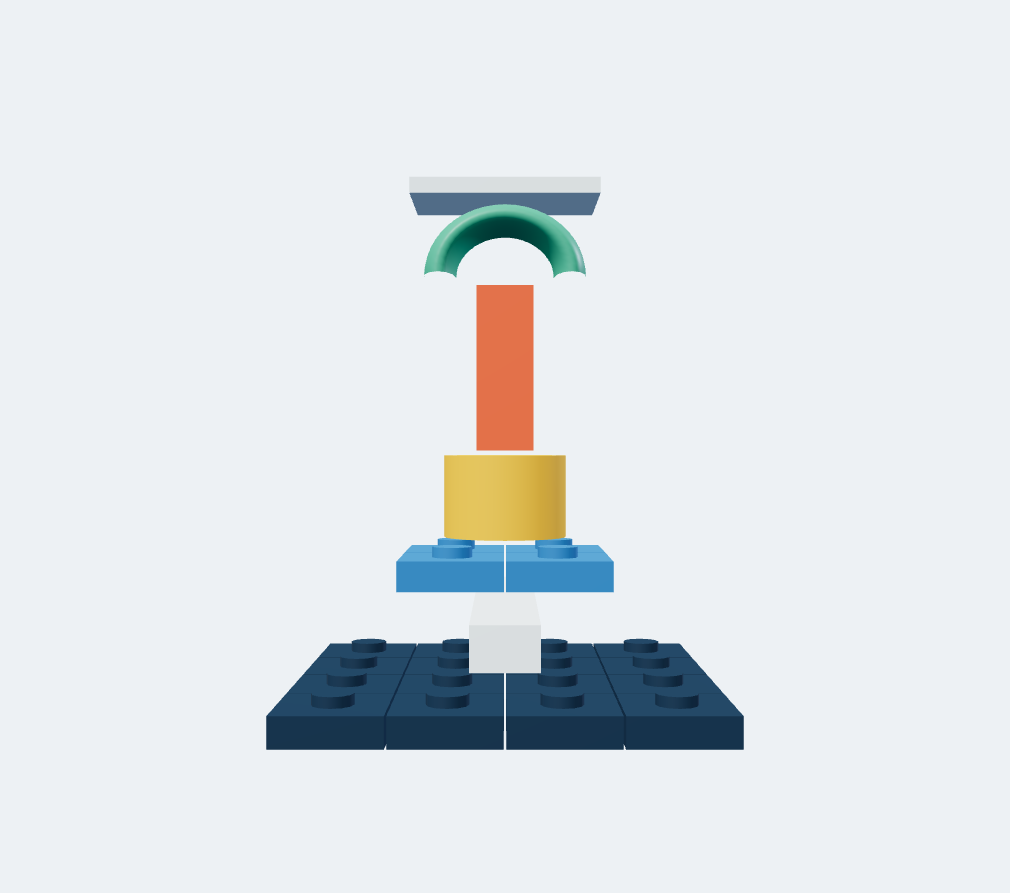
\includegraphics[width=.24\textwidth]{figures/hierarchy3/indexed-toggle-latch-front.png}
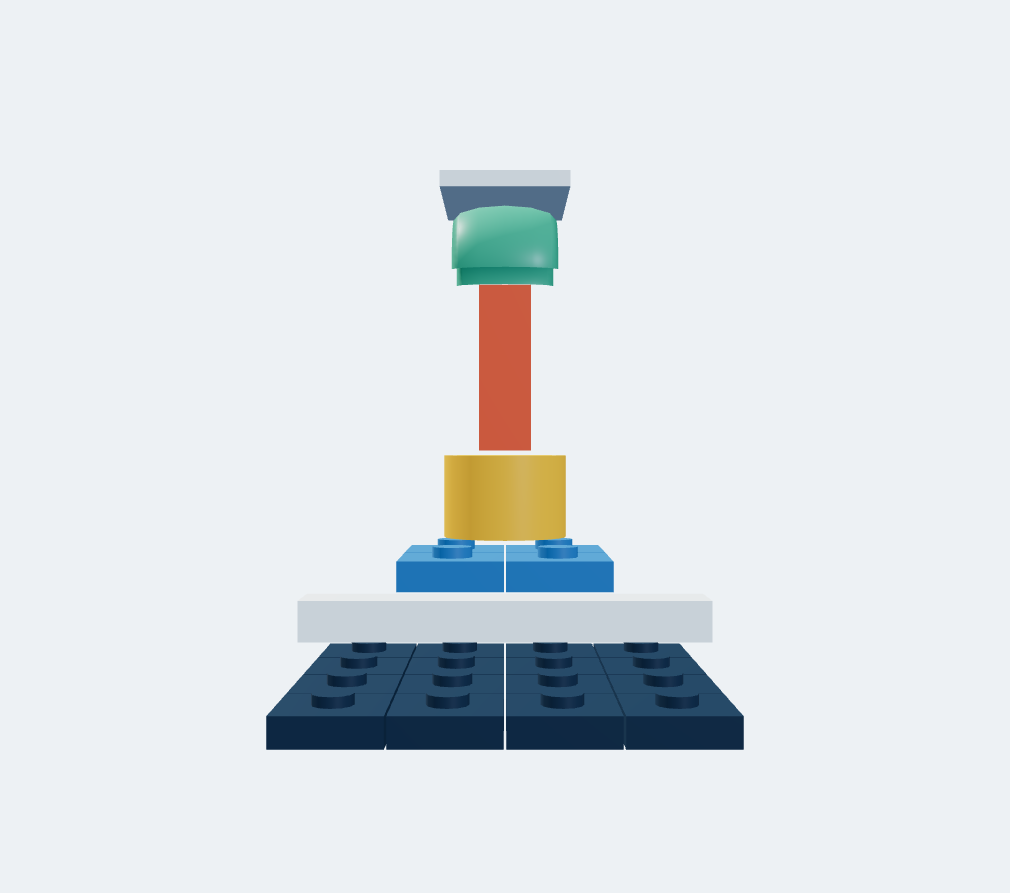
\includegraphics[width=.24\textwidth]{figures/hierarchy3/indexed-toggle-latch-side.png}

\includegraphics[width=.24\textwidth]{figures/hierarchy3/indexed-toggle-latch-top.png}
\end{center}
\noindent All 48 tasks share this source; complete inputs, choices and answers are in the companion question bank.
\begin{center}\tiny\begin{tabular}{rllll}\toprule No. & Family & Layer & Output & Evidence\\\midrule
1 & identify & atomic & single-choice & model-state \\
2 & count & atomic & single-choice & model-state \\
3 & color & atomic & single-choice & model-state \\
4 & position & atomic & single-choice & model-state \\
5 & joint-type & atomic & single-choice & model-state \\
6 & parent & atomic & single-choice & model-state \\
7 & anchor & atomic & single-choice & model-state \\
8 & degree & atomic & single-choice & model-state \\
9 & recolor & atomic & single-choice & model-state \\
10 & add & atomic & single-choice & model-state \\
11 & remove & atomic & single-choice & model-state \\
12 & replace & atomic & single-choice & model-state \\
13 & translate & atomic & single-choice & model-state \\
14 & rotate & atomic & single-choice & model-state \\
15 & next-module & atomic & single-choice & model-state \\
16 & inventory & atomic & single-choice & model-state \\
17 & boundary & atomic & single-choice & model-state \\
18 & no-op & atomic & single-choice & model-state \\
19 & prefix & metacognitive & single-choice & support-graph \\
20 & access & metacognitive & multiple-choice & Rapier \\
21 & counterfactual & metacognitive & single-choice & support-graph \\
22 & dynamic & metacognitive & single-choice & Rapier \\
23 & kinematic & metacognitive & multiple-choice & model-state \\
24 & diagnosis & metacognitive & multiple-choice & model-state \\
25 & information-gain & metacognitive & multiple-choice & finite-world \\
26 & abstention & metacognitive & single-choice & finite-world \\
27 & posterior & metacognitive & single-choice & finite-world \\
28 & pareto & metacognitive & multiple-choice & model-state \\
29 & assembly & procedural & actions & state-machine \\
30 & disassembly & procedural & actions & state-machine \\
31 & service-repair & procedural & actions & state-machine \\
32 & compound-edit & procedural & actions & state-machine \\
33 & multi-fault & integrative & actions & state-machine \\
34 & scheduling & integrative & schedule & resource-schedule \\
35 & policy & integrative & policy & finite-world \\
36 & local-frame & atomic & single-choice & model-state \\
37 & projection & atomic & single-choice & model-state \\
38 & relative-order & atomic & single-choice & model-state \\
39 & joint-axis & atomic & single-choice & model-state \\
40 & clearance-margin & metacognitive & single-choice & model-state \\
41 & load-moment & metacognitive & single-choice & model-state \\
42 & weighted-posterior & metacognitive & single-choice & finite-world \\
43 & expected-loss & metacognitive & single-choice & finite-world \\
44 & trace-threshold & metacognitive & single-choice & Rapier \\
45 & guarded-repair & procedural & actions & state-machine \\
46 & rollback & procedural & actions & state-machine \\
47 & resource-repair & integrative & actions & state-machine \\
48 & budget-policy & integrative & policy & finite-world \\
\bottomrule\end{tabular}\end{center}
\clearpage
\subsection{5. Maintenance Trolley (D1)}
21 visible parts, 5 modules, 4 joints. Nominal representative-point displacement: 0.0000; angular displacement: 0.0000 rad. No inter-module penetration above 0.005, including directly joined modules.
\begin{center}

\includegraphics[width=.24\textwidth]{figures/hierarchy3/maintenance-trolley-iso.png}

\includegraphics[width=.24\textwidth]{figures/hierarchy3/maintenance-trolley-front.png}

\includegraphics[width=.24\textwidth]{figures/hierarchy3/maintenance-trolley-side.png}

\includegraphics[width=.24\textwidth]{figures/hierarchy3/maintenance-trolley-top.png}
\end{center}
\noindent All 48 tasks share this source; complete inputs, choices and answers are in the companion question bank.
\begin{center}\tiny\begin{tabular}{rllll}\toprule No. & Family & Layer & Output & Evidence\\\midrule
1 & identify & atomic & single-choice & model-state \\
2 & count & atomic & single-choice & model-state \\
3 & color & atomic & single-choice & model-state \\
4 & position & atomic & single-choice & model-state \\
5 & joint-type & atomic & single-choice & model-state \\
6 & parent & atomic & single-choice & model-state \\
7 & anchor & atomic & single-choice & model-state \\
8 & degree & atomic & single-choice & model-state \\
9 & recolor & atomic & single-choice & model-state \\
10 & add & atomic & single-choice & model-state \\
11 & remove & atomic & single-choice & model-state \\
12 & replace & atomic & single-choice & model-state \\
13 & translate & atomic & single-choice & model-state \\
14 & rotate & atomic & single-choice & model-state \\
15 & next-module & atomic & single-choice & model-state \\
16 & inventory & atomic & single-choice & model-state \\
17 & boundary & atomic & single-choice & model-state \\
18 & no-op & atomic & single-choice & model-state \\
19 & prefix & metacognitive & single-choice & support-graph \\
20 & access & metacognitive & multiple-choice & Rapier \\
21 & counterfactual & metacognitive & single-choice & support-graph \\
22 & dynamic & metacognitive & single-choice & Rapier \\
23 & kinematic & metacognitive & multiple-choice & model-state \\
24 & diagnosis & metacognitive & multiple-choice & model-state \\
25 & information-gain & metacognitive & multiple-choice & finite-world \\
26 & abstention & metacognitive & single-choice & finite-world \\
27 & posterior & metacognitive & single-choice & finite-world \\
28 & pareto & metacognitive & multiple-choice & model-state \\
29 & assembly & procedural & actions & state-machine \\
30 & disassembly & procedural & actions & state-machine \\
31 & service-repair & procedural & actions & state-machine \\
32 & compound-edit & procedural & actions & state-machine \\
33 & multi-fault & integrative & actions & state-machine \\
34 & scheduling & integrative & schedule & resource-schedule \\
35 & policy & integrative & policy & finite-world \\
36 & local-frame & atomic & single-choice & model-state \\
37 & projection & atomic & single-choice & model-state \\
38 & relative-order & atomic & single-choice & model-state \\
39 & joint-axis & atomic & single-choice & model-state \\
40 & clearance-margin & metacognitive & single-choice & model-state \\
41 & load-moment & metacognitive & single-choice & model-state \\
42 & weighted-posterior & metacognitive & single-choice & finite-world \\
43 & expected-loss & metacognitive & single-choice & finite-world \\
44 & trace-threshold & metacognitive & single-choice & Rapier \\
45 & guarded-repair & procedural & actions & state-machine \\
46 & rollback & procedural & actions & state-machine \\
47 & resource-repair & integrative & actions & state-machine \\
48 & budget-policy & integrative & policy & finite-world \\
\bottomrule\end{tabular}\end{center}
\clearpage
\subsection{6. Orthogonal Probe Stage (D1)}
25 visible parts, 6 modules, 5 joints. Nominal representative-point displacement: 0.0000; angular displacement: 0.0000 rad. No inter-module penetration above 0.005, including directly joined modules.
\begin{center}

\includegraphics[width=.24\textwidth]{figures/hierarchy3/orthogonal-probe-stage-iso.png}
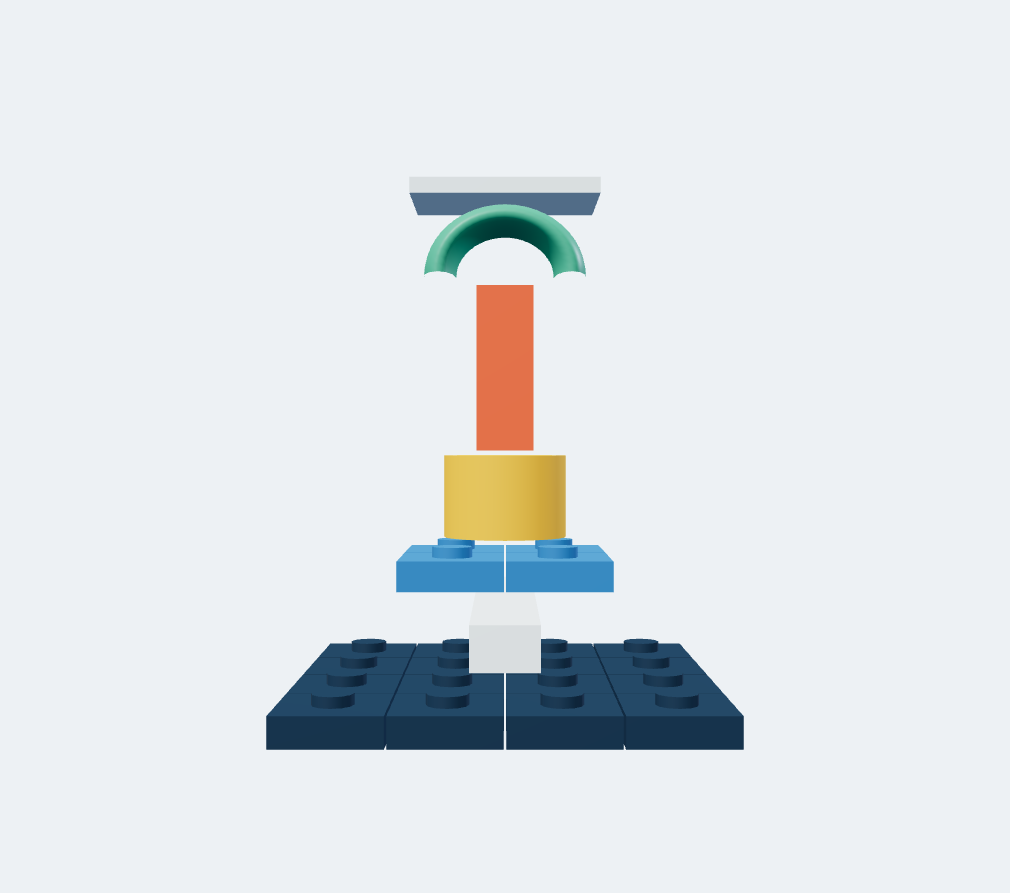
\includegraphics[width=.24\textwidth]{figures/hierarchy3/orthogonal-probe-stage-front.png}
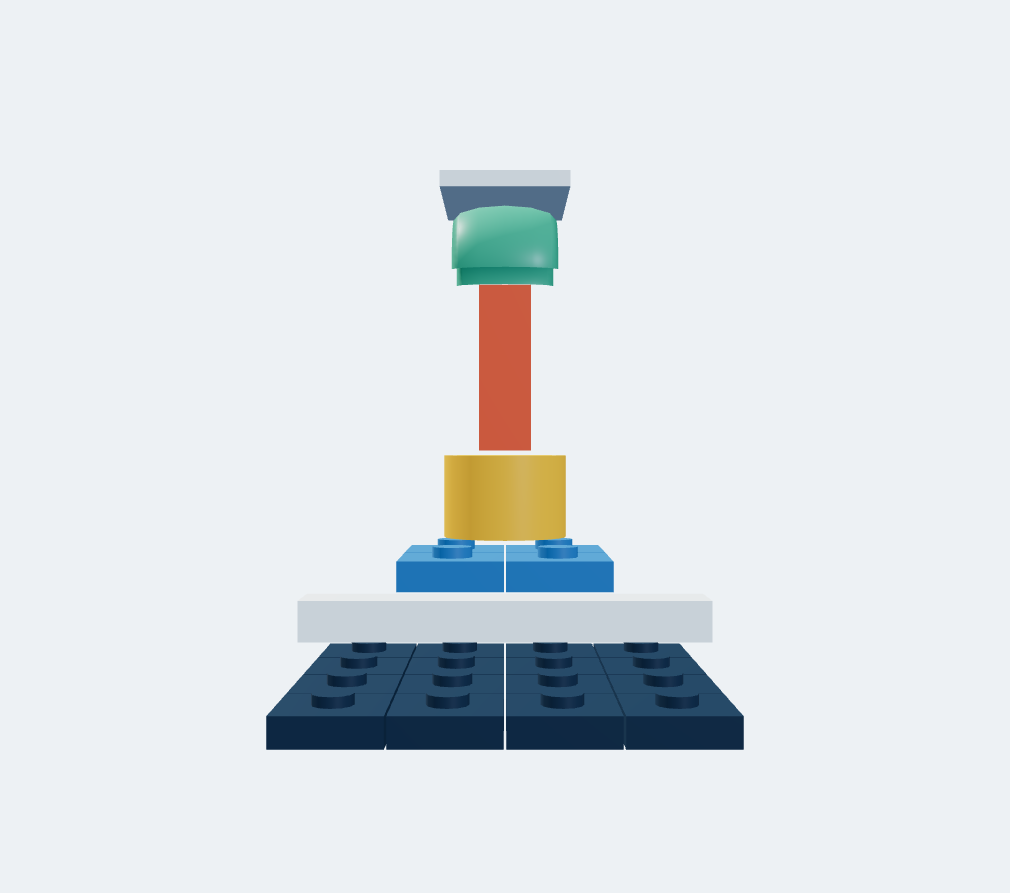
\includegraphics[width=.24\textwidth]{figures/hierarchy3/orthogonal-probe-stage-side.png}

\includegraphics[width=.24\textwidth]{figures/hierarchy3/orthogonal-probe-stage-top.png}
\end{center}
\noindent All 48 tasks share this source; complete inputs, choices and answers are in the companion question bank.
\begin{center}\tiny\begin{tabular}{rllll}\toprule No. & Family & Layer & Output & Evidence\\\midrule
1 & identify & atomic & single-choice & model-state \\
2 & count & atomic & single-choice & model-state \\
3 & color & atomic & single-choice & model-state \\
4 & position & atomic & single-choice & model-state \\
5 & joint-type & atomic & single-choice & model-state \\
6 & parent & atomic & single-choice & model-state \\
7 & anchor & atomic & single-choice & model-state \\
8 & degree & atomic & single-choice & model-state \\
9 & recolor & atomic & single-choice & model-state \\
10 & add & atomic & single-choice & model-state \\
11 & remove & atomic & single-choice & model-state \\
12 & replace & atomic & single-choice & model-state \\
13 & translate & atomic & single-choice & model-state \\
14 & rotate & atomic & single-choice & model-state \\
15 & next-module & atomic & single-choice & model-state \\
16 & inventory & atomic & single-choice & model-state \\
17 & boundary & atomic & single-choice & model-state \\
18 & no-op & atomic & single-choice & model-state \\
19 & prefix & metacognitive & single-choice & support-graph \\
20 & access & metacognitive & multiple-choice & Rapier \\
21 & counterfactual & metacognitive & single-choice & support-graph \\
22 & dynamic & metacognitive & single-choice & Rapier \\
23 & kinematic & metacognitive & multiple-choice & model-state \\
24 & diagnosis & metacognitive & multiple-choice & model-state \\
25 & information-gain & metacognitive & multiple-choice & finite-world \\
26 & abstention & metacognitive & single-choice & finite-world \\
27 & posterior & metacognitive & single-choice & finite-world \\
28 & pareto & metacognitive & multiple-choice & model-state \\
29 & assembly & procedural & actions & state-machine \\
30 & disassembly & procedural & actions & state-machine \\
31 & service-repair & procedural & actions & state-machine \\
32 & compound-edit & procedural & actions & state-machine \\
33 & multi-fault & integrative & actions & state-machine \\
34 & scheduling & integrative & schedule & resource-schedule \\
35 & policy & integrative & policy & finite-world \\
36 & local-frame & atomic & single-choice & model-state \\
37 & projection & atomic & single-choice & model-state \\
38 & relative-order & atomic & single-choice & model-state \\
39 & joint-axis & atomic & single-choice & model-state \\
40 & clearance-margin & metacognitive & single-choice & model-state \\
41 & load-moment & metacognitive & single-choice & model-state \\
42 & weighted-posterior & metacognitive & single-choice & finite-world \\
43 & expected-loss & metacognitive & single-choice & finite-world \\
44 & trace-threshold & metacognitive & single-choice & Rapier \\
45 & guarded-repair & procedural & actions & state-machine \\
46 & rollback & procedural & actions & state-machine \\
47 & resource-repair & integrative & actions & state-machine \\
48 & budget-policy & integrative & policy & finite-world \\
\bottomrule\end{tabular}\end{center}
\clearpage
\subsection{7. Ratchet Hoist (D1)}
16 visible parts, 4 modules, 3 joints. Nominal representative-point displacement: 0.0006; angular displacement: 0.0000 rad. No inter-module penetration above 0.005, including directly joined modules.
\begin{center}

\includegraphics[width=.24\textwidth]{figures/hierarchy3/ratchet-hoist-iso.png}

\includegraphics[width=.24\textwidth]{figures/hierarchy3/ratchet-hoist-front.png}

\includegraphics[width=.24\textwidth]{figures/hierarchy3/ratchet-hoist-side.png}

\includegraphics[width=.24\textwidth]{figures/hierarchy3/ratchet-hoist-top.png}
\end{center}
\noindent All 48 tasks share this source; complete inputs, choices and answers are in the companion question bank.
\begin{center}\tiny\begin{tabular}{rllll}\toprule No. & Family & Layer & Output & Evidence\\\midrule
1 & identify & atomic & single-choice & model-state \\
2 & count & atomic & single-choice & model-state \\
3 & color & atomic & single-choice & model-state \\
4 & position & atomic & single-choice & model-state \\
5 & joint-type & atomic & single-choice & model-state \\
6 & parent & atomic & single-choice & model-state \\
7 & anchor & atomic & single-choice & model-state \\
8 & degree & atomic & single-choice & model-state \\
9 & recolor & atomic & single-choice & model-state \\
10 & add & atomic & single-choice & model-state \\
11 & remove & atomic & single-choice & model-state \\
12 & replace & atomic & single-choice & model-state \\
13 & translate & atomic & single-choice & model-state \\
14 & rotate & atomic & single-choice & model-state \\
15 & next-module & atomic & single-choice & model-state \\
16 & inventory & atomic & single-choice & model-state \\
17 & boundary & atomic & single-choice & model-state \\
18 & no-op & atomic & single-choice & model-state \\
19 & prefix & metacognitive & single-choice & support-graph \\
20 & access & metacognitive & multiple-choice & Rapier \\
21 & counterfactual & metacognitive & single-choice & support-graph \\
22 & dynamic & metacognitive & single-choice & Rapier \\
23 & kinematic & metacognitive & multiple-choice & model-state \\
24 & diagnosis & metacognitive & multiple-choice & model-state \\
25 & information-gain & metacognitive & multiple-choice & finite-world \\
26 & abstention & metacognitive & single-choice & finite-world \\
27 & posterior & metacognitive & single-choice & finite-world \\
28 & pareto & metacognitive & multiple-choice & model-state \\
29 & assembly & procedural & actions & state-machine \\
30 & disassembly & procedural & actions & state-machine \\
31 & service-repair & procedural & actions & state-machine \\
32 & compound-edit & procedural & actions & state-machine \\
33 & multi-fault & integrative & actions & state-machine \\
34 & scheduling & integrative & schedule & resource-schedule \\
35 & policy & integrative & policy & finite-world \\
36 & local-frame & atomic & single-choice & model-state \\
37 & projection & atomic & single-choice & model-state \\
38 & relative-order & atomic & single-choice & model-state \\
39 & joint-axis & atomic & single-choice & model-state \\
40 & clearance-margin & metacognitive & single-choice & model-state \\
41 & load-moment & metacognitive & single-choice & model-state \\
42 & weighted-posterior & metacognitive & single-choice & finite-world \\
43 & expected-loss & metacognitive & single-choice & finite-world \\
44 & trace-threshold & metacognitive & single-choice & Rapier \\
45 & guarded-repair & procedural & actions & state-machine \\
46 & rollback & procedural & actions & state-machine \\
47 & resource-repair & integrative & actions & state-machine \\
48 & budget-policy & integrative & policy & finite-world \\
\bottomrule\end{tabular}\end{center}
\clearpage
\subsection{8. Sample Carousel (D1)}
15 visible parts, 4 modules, 3 joints. Nominal representative-point displacement: 0.0000; angular displacement: 0.0000 rad. No inter-module penetration above 0.005, including directly joined modules.
\begin{center}

\includegraphics[width=.24\textwidth]{figures/hierarchy3/sample-carousel-iso.png}

\includegraphics[width=.24\textwidth]{figures/hierarchy3/sample-carousel-front.png}

\includegraphics[width=.24\textwidth]{figures/hierarchy3/sample-carousel-side.png}

\includegraphics[width=.24\textwidth]{figures/hierarchy3/sample-carousel-top.png}
\end{center}
\noindent All 48 tasks share this source; complete inputs, choices and answers are in the companion question bank.
\begin{center}\tiny\begin{tabular}{rllll}\toprule No. & Family & Layer & Output & Evidence\\\midrule
1 & identify & atomic & single-choice & model-state \\
2 & count & atomic & single-choice & model-state \\
3 & color & atomic & single-choice & model-state \\
4 & position & atomic & single-choice & model-state \\
5 & joint-type & atomic & single-choice & model-state \\
6 & parent & atomic & single-choice & model-state \\
7 & anchor & atomic & single-choice & model-state \\
8 & degree & atomic & single-choice & model-state \\
9 & recolor & atomic & single-choice & model-state \\
10 & add & atomic & single-choice & model-state \\
11 & remove & atomic & single-choice & model-state \\
12 & replace & atomic & single-choice & model-state \\
13 & translate & atomic & single-choice & model-state \\
14 & rotate & atomic & single-choice & model-state \\
15 & next-module & atomic & single-choice & model-state \\
16 & inventory & atomic & single-choice & model-state \\
17 & boundary & atomic & single-choice & model-state \\
18 & no-op & atomic & single-choice & model-state \\
19 & prefix & metacognitive & single-choice & support-graph \\
20 & access & metacognitive & multiple-choice & Rapier \\
21 & counterfactual & metacognitive & single-choice & support-graph \\
22 & dynamic & metacognitive & single-choice & Rapier \\
23 & kinematic & metacognitive & multiple-choice & model-state \\
24 & diagnosis & metacognitive & multiple-choice & model-state \\
25 & information-gain & metacognitive & multiple-choice & finite-world \\
26 & abstention & metacognitive & single-choice & finite-world \\
27 & posterior & metacognitive & single-choice & finite-world \\
28 & pareto & metacognitive & multiple-choice & model-state \\
29 & assembly & procedural & actions & state-machine \\
30 & disassembly & procedural & actions & state-machine \\
31 & service-repair & procedural & actions & state-machine \\
32 & compound-edit & procedural & actions & state-machine \\
33 & multi-fault & integrative & actions & state-machine \\
34 & scheduling & integrative & schedule & resource-schedule \\
35 & policy & integrative & policy & finite-world \\
36 & local-frame & atomic & single-choice & model-state \\
37 & projection & atomic & single-choice & model-state \\
38 & relative-order & atomic & single-choice & model-state \\
39 & joint-axis & atomic & single-choice & model-state \\
40 & clearance-margin & metacognitive & single-choice & model-state \\
41 & load-moment & metacognitive & single-choice & model-state \\
42 & weighted-posterior & metacognitive & single-choice & finite-world \\
43 & expected-loss & metacognitive & single-choice & finite-world \\
44 & trace-threshold & metacognitive & single-choice & Rapier \\
45 & guarded-repair & procedural & actions & state-machine \\
46 & rollback & procedural & actions & state-machine \\
47 & resource-repair & integrative & actions & state-machine \\
48 & budget-policy & integrative & policy & finite-world \\
\bottomrule\end{tabular}\end{center}
\clearpage
\subsection{9. Signal Switch Stand (D1)}
22 visible parts, 4 modules, 3 joints. Nominal representative-point displacement: 0.0035; angular displacement: 0.0000 rad. No inter-module penetration above 0.005, including directly joined modules.
\begin{center}

\includegraphics[width=.24\textwidth]{figures/hierarchy3/signal-switch-stand-iso.png}

\includegraphics[width=.24\textwidth]{figures/hierarchy3/signal-switch-stand-front.png}

\includegraphics[width=.24\textwidth]{figures/hierarchy3/signal-switch-stand-side.png}

\includegraphics[width=.24\textwidth]{figures/hierarchy3/signal-switch-stand-top.png}
\end{center}
\noindent All 48 tasks share this source; complete inputs, choices and answers are in the companion question bank.
\begin{center}\tiny\begin{tabular}{rllll}\toprule No. & Family & Layer & Output & Evidence\\\midrule
1 & identify & atomic & single-choice & model-state \\
2 & count & atomic & single-choice & model-state \\
3 & color & atomic & single-choice & model-state \\
4 & position & atomic & single-choice & model-state \\
5 & joint-type & atomic & single-choice & model-state \\
6 & parent & atomic & single-choice & model-state \\
7 & anchor & atomic & single-choice & model-state \\
8 & degree & atomic & single-choice & model-state \\
9 & recolor & atomic & single-choice & model-state \\
10 & add & atomic & single-choice & model-state \\
11 & remove & atomic & single-choice & model-state \\
12 & replace & atomic & single-choice & model-state \\
13 & translate & atomic & single-choice & model-state \\
14 & rotate & atomic & single-choice & model-state \\
15 & next-module & atomic & single-choice & model-state \\
16 & inventory & atomic & single-choice & model-state \\
17 & boundary & atomic & single-choice & model-state \\
18 & no-op & atomic & single-choice & model-state \\
19 & prefix & metacognitive & single-choice & support-graph \\
20 & access & metacognitive & multiple-choice & Rapier \\
21 & counterfactual & metacognitive & single-choice & support-graph \\
22 & dynamic & metacognitive & single-choice & Rapier \\
23 & kinematic & metacognitive & multiple-choice & model-state \\
24 & diagnosis & metacognitive & multiple-choice & model-state \\
25 & information-gain & metacognitive & multiple-choice & finite-world \\
26 & abstention & metacognitive & single-choice & finite-world \\
27 & posterior & metacognitive & single-choice & finite-world \\
28 & pareto & metacognitive & multiple-choice & model-state \\
29 & assembly & procedural & actions & state-machine \\
30 & disassembly & procedural & actions & state-machine \\
31 & service-repair & procedural & actions & state-machine \\
32 & compound-edit & procedural & actions & state-machine \\
33 & multi-fault & integrative & actions & state-machine \\
34 & scheduling & integrative & schedule & resource-schedule \\
35 & policy & integrative & policy & finite-world \\
36 & local-frame & atomic & single-choice & model-state \\
37 & projection & atomic & single-choice & model-state \\
38 & relative-order & atomic & single-choice & model-state \\
39 & joint-axis & atomic & single-choice & model-state \\
40 & clearance-margin & metacognitive & single-choice & model-state \\
41 & load-moment & metacognitive & single-choice & model-state \\
42 & weighted-posterior & metacognitive & single-choice & finite-world \\
43 & expected-loss & metacognitive & single-choice & finite-world \\
44 & trace-threshold & metacognitive & single-choice & Rapier \\
45 & guarded-repair & procedural & actions & state-machine \\
46 & rollback & procedural & actions & state-machine \\
47 & resource-repair & integrative & actions & state-machine \\
48 & budget-policy & integrative & policy & finite-world \\
\bottomrule\end{tabular}\end{center}
\clearpage
\subsection{10. Rail Tool Drawer (D1)}
17 visible parts, 4 modules, 3 joints. Nominal representative-point displacement: 0.0000; angular displacement: 0.0000 rad. No inter-module penetration above 0.005, including directly joined modules.
\begin{center}

\includegraphics[width=.24\textwidth]{figures/hierarchy3/sliding-drawer-iso.png}

\includegraphics[width=.24\textwidth]{figures/hierarchy3/sliding-drawer-front.png}

\includegraphics[width=.24\textwidth]{figures/hierarchy3/sliding-drawer-side.png}

\includegraphics[width=.24\textwidth]{figures/hierarchy3/sliding-drawer-top.png}
\end{center}
\noindent All 48 tasks share this source; complete inputs, choices and answers are in the companion question bank.
\begin{center}\tiny\begin{tabular}{rllll}\toprule No. & Family & Layer & Output & Evidence\\\midrule
1 & identify & atomic & single-choice & model-state \\
2 & count & atomic & single-choice & model-state \\
3 & color & atomic & single-choice & model-state \\
4 & position & atomic & single-choice & model-state \\
5 & joint-type & atomic & single-choice & model-state \\
6 & parent & atomic & single-choice & model-state \\
7 & anchor & atomic & single-choice & model-state \\
8 & degree & atomic & single-choice & model-state \\
9 & recolor & atomic & single-choice & model-state \\
10 & add & atomic & single-choice & model-state \\
11 & remove & atomic & single-choice & model-state \\
12 & replace & atomic & single-choice & model-state \\
13 & translate & atomic & single-choice & model-state \\
14 & rotate & atomic & single-choice & model-state \\
15 & next-module & atomic & single-choice & model-state \\
16 & inventory & atomic & single-choice & model-state \\
17 & boundary & atomic & single-choice & model-state \\
18 & no-op & atomic & single-choice & model-state \\
19 & prefix & metacognitive & single-choice & support-graph \\
20 & access & metacognitive & multiple-choice & Rapier \\
21 & counterfactual & metacognitive & single-choice & support-graph \\
22 & dynamic & metacognitive & single-choice & Rapier \\
23 & kinematic & metacognitive & multiple-choice & model-state \\
24 & diagnosis & metacognitive & multiple-choice & model-state \\
25 & information-gain & metacognitive & multiple-choice & finite-world \\
26 & abstention & metacognitive & single-choice & finite-world \\
27 & posterior & metacognitive & single-choice & finite-world \\
28 & pareto & metacognitive & multiple-choice & model-state \\
29 & assembly & procedural & actions & state-machine \\
30 & disassembly & procedural & actions & state-machine \\
31 & service-repair & procedural & actions & state-machine \\
32 & compound-edit & procedural & actions & state-machine \\
33 & multi-fault & integrative & actions & state-machine \\
34 & scheduling & integrative & schedule & resource-schedule \\
35 & policy & integrative & policy & finite-world \\
36 & local-frame & atomic & single-choice & model-state \\
37 & projection & atomic & single-choice & model-state \\
38 & relative-order & atomic & single-choice & model-state \\
39 & joint-axis & atomic & single-choice & model-state \\
40 & clearance-margin & metacognitive & single-choice & model-state \\
41 & load-moment & metacognitive & single-choice & model-state \\
42 & weighted-posterior & metacognitive & single-choice & finite-world \\
43 & expected-loss & metacognitive & single-choice & finite-world \\
44 & trace-threshold & metacognitive & single-choice & Rapier \\
45 & guarded-repair & procedural & actions & state-machine \\
46 & rollback & procedural & actions & state-machine \\
47 & resource-repair & integrative & actions & state-machine \\
48 & budget-policy & integrative & policy & finite-world \\
\bottomrule\end{tabular}\end{center}
\clearpage
\subsection{11. Valve Control Stand (D1)}
25 visible parts, 3 modules, 2 joints. Nominal representative-point displacement: 0.0000; angular displacement: 0.0000 rad. No inter-module penetration above 0.005, including directly joined modules.
\begin{center}

\includegraphics[width=.24\textwidth]{figures/hierarchy3/valve-control-stand-iso.png}

\includegraphics[width=.24\textwidth]{figures/hierarchy3/valve-control-stand-front.png}

\includegraphics[width=.24\textwidth]{figures/hierarchy3/valve-control-stand-side.png}

\includegraphics[width=.24\textwidth]{figures/hierarchy3/valve-control-stand-top.png}
\end{center}
\noindent All 48 tasks share this source; complete inputs, choices and answers are in the companion question bank.
\begin{center}\tiny\begin{tabular}{rllll}\toprule No. & Family & Layer & Output & Evidence\\\midrule
1 & identify & atomic & single-choice & model-state \\
2 & count & atomic & single-choice & model-state \\
3 & color & atomic & single-choice & model-state \\
4 & position & atomic & single-choice & model-state \\
5 & joint-type & atomic & single-choice & model-state \\
6 & parent & atomic & single-choice & model-state \\
7 & anchor & atomic & single-choice & model-state \\
8 & degree & atomic & single-choice & model-state \\
9 & recolor & atomic & single-choice & model-state \\
10 & add & atomic & single-choice & model-state \\
11 & remove & atomic & single-choice & model-state \\
12 & replace & atomic & single-choice & model-state \\
13 & translate & atomic & single-choice & model-state \\
14 & rotate & atomic & single-choice & model-state \\
15 & next-module & atomic & single-choice & model-state \\
16 & inventory & atomic & single-choice & model-state \\
17 & boundary & atomic & single-choice & model-state \\
18 & no-op & atomic & single-choice & model-state \\
19 & prefix & metacognitive & single-choice & support-graph \\
20 & access & metacognitive & multiple-choice & Rapier \\
21 & counterfactual & metacognitive & single-choice & support-graph \\
22 & dynamic & metacognitive & single-choice & Rapier \\
23 & kinematic & metacognitive & multiple-choice & model-state \\
24 & diagnosis & metacognitive & multiple-choice & model-state \\
25 & information-gain & metacognitive & multiple-choice & finite-world \\
26 & abstention & metacognitive & single-choice & finite-world \\
27 & posterior & metacognitive & single-choice & finite-world \\
28 & pareto & metacognitive & multiple-choice & model-state \\
29 & assembly & procedural & actions & state-machine \\
30 & disassembly & procedural & actions & state-machine \\
31 & service-repair & procedural & actions & state-machine \\
32 & compound-edit & procedural & actions & state-machine \\
33 & multi-fault & integrative & actions & state-machine \\
34 & scheduling & integrative & schedule & resource-schedule \\
35 & policy & integrative & policy & finite-world \\
36 & local-frame & atomic & single-choice & model-state \\
37 & projection & atomic & single-choice & model-state \\
38 & relative-order & atomic & single-choice & model-state \\
39 & joint-axis & atomic & single-choice & model-state \\
40 & clearance-margin & metacognitive & single-choice & model-state \\
41 & load-moment & metacognitive & single-choice & model-state \\
42 & weighted-posterior & metacognitive & single-choice & finite-world \\
43 & expected-loss & metacognitive & single-choice & finite-world \\
44 & trace-threshold & metacognitive & single-choice & Rapier \\
45 & guarded-repair & procedural & actions & state-machine \\
46 & rollback & procedural & actions & state-machine \\
47 & resource-repair & integrative & actions & state-machine \\
48 & budget-policy & integrative & policy & finite-world \\
\bottomrule\end{tabular}\end{center}
\clearpage
\subsection{12. Wind Vane (D1)}
14 visible parts, 4 modules, 3 joints. Nominal representative-point displacement: 0.0000; angular displacement: 0.0000 rad. No inter-module penetration above 0.005, including directly joined modules.
\begin{center}

\includegraphics[width=.24\textwidth]{figures/hierarchy3/wind-vane-iso.png}

\includegraphics[width=.24\textwidth]{figures/hierarchy3/wind-vane-front.png}

\includegraphics[width=.24\textwidth]{figures/hierarchy3/wind-vane-side.png}

\includegraphics[width=.24\textwidth]{figures/hierarchy3/wind-vane-top.png}
\end{center}
\noindent All 48 tasks share this source; complete inputs, choices and answers are in the companion question bank.
\begin{center}\tiny\begin{tabular}{rllll}\toprule No. & Family & Layer & Output & Evidence\\\midrule
1 & identify & atomic & single-choice & model-state \\
2 & count & atomic & single-choice & model-state \\
3 & color & atomic & single-choice & model-state \\
4 & position & atomic & single-choice & model-state \\
5 & joint-type & atomic & single-choice & model-state \\
6 & parent & atomic & single-choice & model-state \\
7 & anchor & atomic & single-choice & model-state \\
8 & degree & atomic & single-choice & model-state \\
9 & recolor & atomic & single-choice & model-state \\
10 & add & atomic & single-choice & model-state \\
11 & remove & atomic & single-choice & model-state \\
12 & replace & atomic & single-choice & model-state \\
13 & translate & atomic & single-choice & model-state \\
14 & rotate & atomic & single-choice & model-state \\
15 & next-module & atomic & single-choice & model-state \\
16 & inventory & atomic & single-choice & model-state \\
17 & boundary & atomic & single-choice & model-state \\
18 & no-op & atomic & single-choice & model-state \\
19 & prefix & metacognitive & single-choice & support-graph \\
20 & access & metacognitive & multiple-choice & Rapier \\
21 & counterfactual & metacognitive & single-choice & support-graph \\
22 & dynamic & metacognitive & single-choice & Rapier \\
23 & kinematic & metacognitive & multiple-choice & model-state \\
24 & diagnosis & metacognitive & multiple-choice & model-state \\
25 & information-gain & metacognitive & multiple-choice & finite-world \\
26 & abstention & metacognitive & single-choice & finite-world \\
27 & posterior & metacognitive & single-choice & finite-world \\
28 & pareto & metacognitive & multiple-choice & model-state \\
29 & assembly & procedural & actions & state-machine \\
30 & disassembly & procedural & actions & state-machine \\
31 & service-repair & procedural & actions & state-machine \\
32 & compound-edit & procedural & actions & state-machine \\
33 & multi-fault & integrative & actions & state-machine \\
34 & scheduling & integrative & schedule & resource-schedule \\
35 & policy & integrative & policy & finite-world \\
36 & local-frame & atomic & single-choice & model-state \\
37 & projection & atomic & single-choice & model-state \\
38 & relative-order & atomic & single-choice & model-state \\
39 & joint-axis & atomic & single-choice & model-state \\
40 & clearance-margin & metacognitive & single-choice & model-state \\
41 & load-moment & metacognitive & single-choice & model-state \\
42 & weighted-posterior & metacognitive & single-choice & finite-world \\
43 & expected-loss & metacognitive & single-choice & finite-world \\
44 & trace-threshold & metacognitive & single-choice & Rapier \\
45 & guarded-repair & procedural & actions & state-machine \\
46 & rollback & procedural & actions & state-machine \\
47 & resource-repair & integrative & actions & state-machine \\
48 & budget-policy & integrative & policy & finite-world \\
\bottomrule\end{tabular}\end{center}
\clearpage
\subsection{13. Articulated Camera Dolly (D2)}
54 visible parts, 11 modules, 10 joints. Nominal representative-point displacement: 0.0000; angular displacement: 0.0000 rad. No inter-module penetration above 0.005, including directly joined modules.
\begin{center}
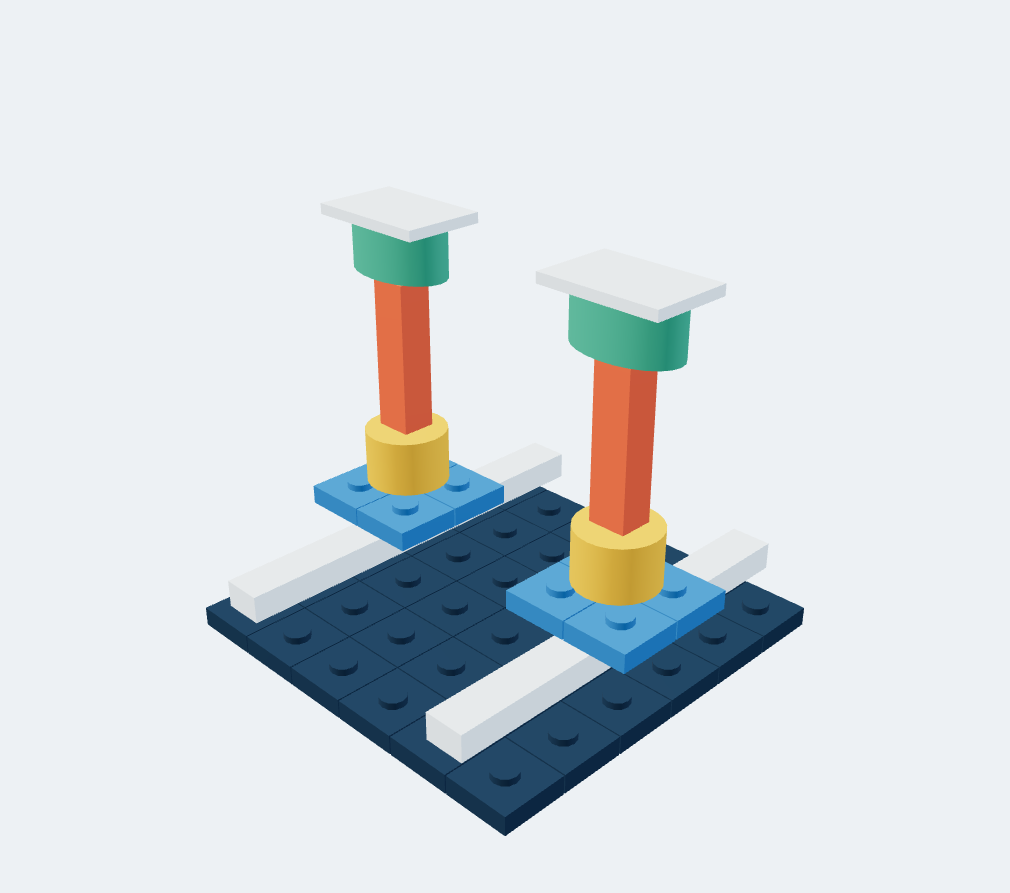
\includegraphics[width=.24\textwidth]{figures/hierarchy3/articulated-camera-dolly-iso.png}
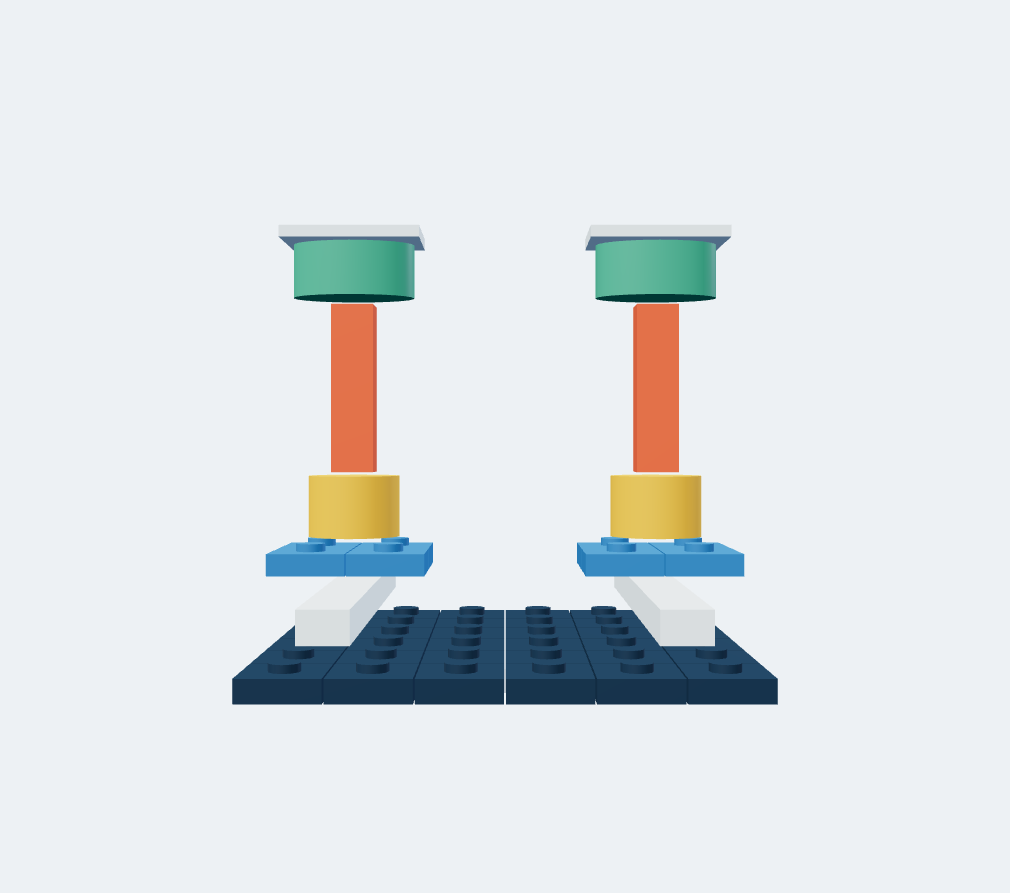
\includegraphics[width=.24\textwidth]{figures/hierarchy3/articulated-camera-dolly-front.png}
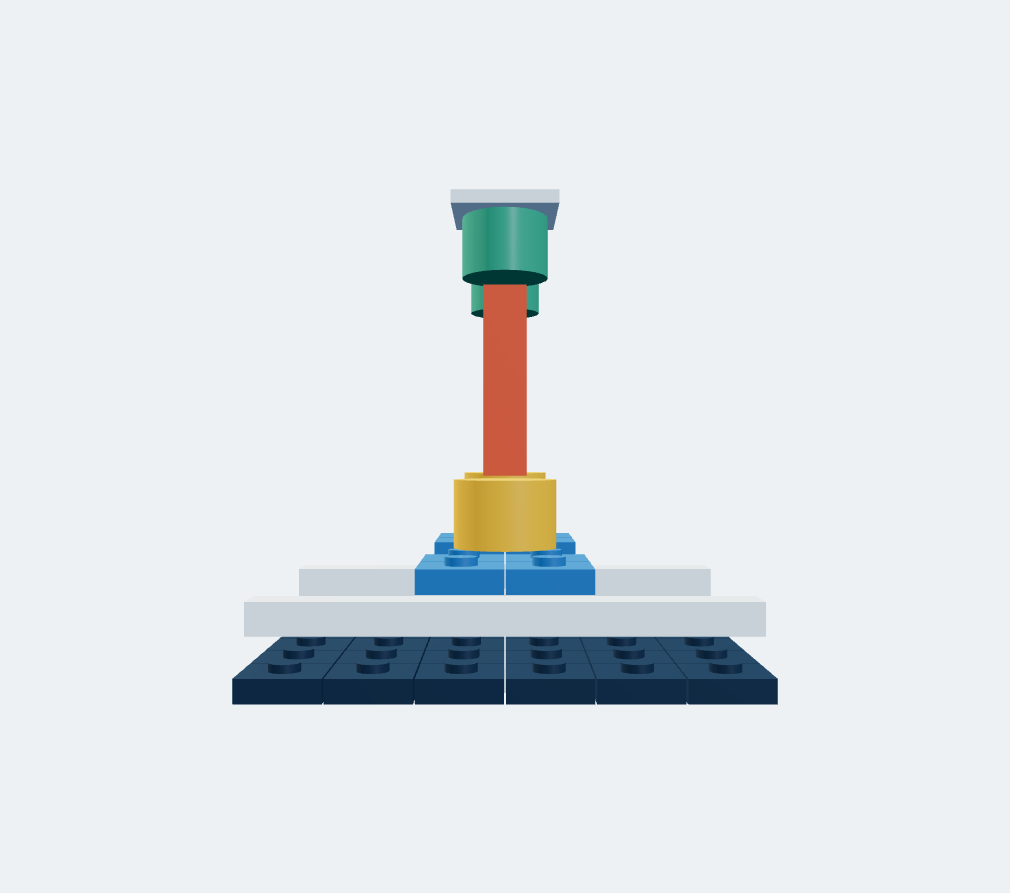
\includegraphics[width=.24\textwidth]{figures/hierarchy3/articulated-camera-dolly-side.png}
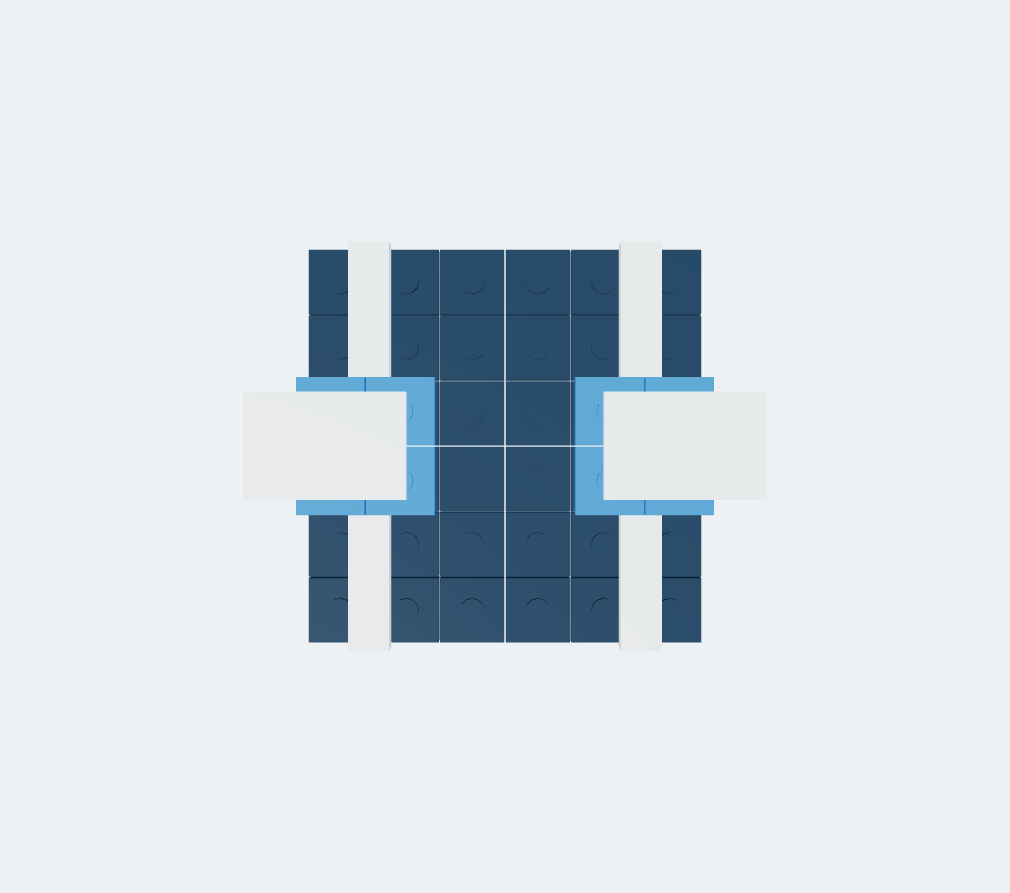
\includegraphics[width=.24\textwidth]{figures/hierarchy3/articulated-camera-dolly-top.png}
\end{center}
\noindent All 48 tasks share this source; complete inputs, choices and answers are in the companion question bank.
\begin{center}\tiny\begin{tabular}{rllll}\toprule No. & Family & Layer & Output & Evidence\\\midrule
1 & identify & atomic & single-choice & model-state \\
2 & count & atomic & single-choice & model-state \\
3 & color & atomic & single-choice & model-state \\
4 & position & atomic & single-choice & model-state \\
5 & joint-type & atomic & single-choice & model-state \\
6 & parent & atomic & single-choice & model-state \\
7 & anchor & atomic & single-choice & model-state \\
8 & degree & atomic & single-choice & model-state \\
9 & recolor & atomic & single-choice & model-state \\
10 & add & atomic & single-choice & model-state \\
11 & remove & atomic & single-choice & model-state \\
12 & replace & atomic & single-choice & model-state \\
13 & translate & atomic & single-choice & model-state \\
14 & rotate & atomic & single-choice & model-state \\
15 & next-module & atomic & single-choice & model-state \\
16 & inventory & atomic & single-choice & model-state \\
17 & boundary & atomic & single-choice & model-state \\
18 & no-op & atomic & single-choice & model-state \\
19 & prefix & metacognitive & single-choice & support-graph \\
20 & access & metacognitive & multiple-choice & Rapier \\
21 & counterfactual & metacognitive & single-choice & support-graph \\
22 & dynamic & metacognitive & single-choice & Rapier \\
23 & kinematic & metacognitive & multiple-choice & model-state \\
24 & diagnosis & metacognitive & multiple-choice & model-state \\
25 & information-gain & metacognitive & multiple-choice & finite-world \\
26 & abstention & metacognitive & single-choice & finite-world \\
27 & posterior & metacognitive & single-choice & finite-world \\
28 & pareto & metacognitive & multiple-choice & model-state \\
29 & assembly & procedural & actions & state-machine \\
30 & disassembly & procedural & actions & state-machine \\
31 & service-repair & procedural & actions & state-machine \\
32 & compound-edit & procedural & actions & state-machine \\
33 & multi-fault & integrative & actions & state-machine \\
34 & scheduling & integrative & schedule & resource-schedule \\
35 & policy & integrative & policy & finite-world \\
36 & local-frame & atomic & single-choice & model-state \\
37 & projection & atomic & single-choice & model-state \\
38 & relative-order & atomic & single-choice & model-state \\
39 & joint-axis & atomic & single-choice & model-state \\
40 & clearance-margin & metacognitive & single-choice & model-state \\
41 & load-moment & metacognitive & single-choice & model-state \\
42 & weighted-posterior & metacognitive & single-choice & finite-world \\
43 & expected-loss & metacognitive & single-choice & finite-world \\
44 & trace-threshold & metacognitive & single-choice & Rapier \\
45 & guarded-repair & procedural & actions & state-machine \\
46 & rollback & procedural & actions & state-machine \\
47 & resource-repair & integrative & actions & state-machine \\
48 & budget-policy & integrative & policy & finite-world \\
\bottomrule\end{tabular}\end{center}
\clearpage
\subsection{14. Articulated Loader (D2)}
126 visible parts, 8 modules, 7 joints. Nominal representative-point displacement: 0.0100; angular displacement: 0.0017 rad. No inter-module penetration above 0.005, including directly joined modules.
\begin{center}

\includegraphics[width=.24\textwidth]{figures/hierarchy3/articulated-loader-iso.png}

\includegraphics[width=.24\textwidth]{figures/hierarchy3/articulated-loader-front.png}

\includegraphics[width=.24\textwidth]{figures/hierarchy3/articulated-loader-side.png}

\includegraphics[width=.24\textwidth]{figures/hierarchy3/articulated-loader-top.png}
\end{center}
\noindent All 48 tasks share this source; complete inputs, choices and answers are in the companion question bank.
\begin{center}\tiny\begin{tabular}{rllll}\toprule No. & Family & Layer & Output & Evidence\\\midrule
1 & identify & atomic & single-choice & model-state \\
2 & count & atomic & single-choice & model-state \\
3 & color & atomic & single-choice & model-state \\
4 & position & atomic & single-choice & model-state \\
5 & joint-type & atomic & single-choice & model-state \\
6 & parent & atomic & single-choice & model-state \\
7 & anchor & atomic & single-choice & model-state \\
8 & degree & atomic & single-choice & model-state \\
9 & recolor & atomic & single-choice & model-state \\
10 & add & atomic & single-choice & model-state \\
11 & remove & atomic & single-choice & model-state \\
12 & replace & atomic & single-choice & model-state \\
13 & translate & atomic & single-choice & model-state \\
14 & rotate & atomic & single-choice & model-state \\
15 & next-module & atomic & single-choice & model-state \\
16 & inventory & atomic & single-choice & model-state \\
17 & boundary & atomic & single-choice & model-state \\
18 & no-op & atomic & single-choice & model-state \\
19 & prefix & metacognitive & single-choice & support-graph \\
20 & access & metacognitive & multiple-choice & Rapier \\
21 & counterfactual & metacognitive & single-choice & support-graph \\
22 & dynamic & metacognitive & single-choice & Rapier \\
23 & kinematic & metacognitive & multiple-choice & model-state \\
24 & diagnosis & metacognitive & multiple-choice & model-state \\
25 & information-gain & metacognitive & multiple-choice & finite-world \\
26 & abstention & metacognitive & single-choice & finite-world \\
27 & posterior & metacognitive & single-choice & finite-world \\
28 & pareto & metacognitive & multiple-choice & model-state \\
29 & assembly & procedural & actions & state-machine \\
30 & disassembly & procedural & actions & state-machine \\
31 & service-repair & procedural & actions & state-machine \\
32 & compound-edit & procedural & actions & state-machine \\
33 & multi-fault & integrative & actions & state-machine \\
34 & scheduling & integrative & schedule & resource-schedule \\
35 & policy & integrative & policy & finite-world \\
36 & local-frame & atomic & single-choice & model-state \\
37 & projection & atomic & single-choice & model-state \\
38 & relative-order & atomic & single-choice & model-state \\
39 & joint-axis & atomic & single-choice & model-state \\
40 & clearance-margin & metacognitive & single-choice & model-state \\
41 & load-moment & metacognitive & single-choice & model-state \\
42 & weighted-posterior & metacognitive & single-choice & finite-world \\
43 & expected-loss & metacognitive & single-choice & finite-world \\
44 & trace-threshold & metacognitive & single-choice & Rapier \\
45 & guarded-repair & procedural & actions & state-machine \\
46 & rollback & procedural & actions & state-machine \\
47 & resource-repair & integrative & actions & state-machine \\
48 & budget-policy & integrative & policy & finite-world \\
\bottomrule\end{tabular}\end{center}
\clearpage
\subsection{15. Canal Inspection Skiff (D2)}
45 visible parts, 5 modules, 4 joints. Nominal representative-point displacement: 0.0000; angular displacement: 0.0000 rad. No inter-module penetration above 0.005, including directly joined modules.
\begin{center}

\includegraphics[width=.24\textwidth]{figures/hierarchy3/canal-inspection-skiff-iso.png}

\includegraphics[width=.24\textwidth]{figures/hierarchy3/canal-inspection-skiff-front.png}

\includegraphics[width=.24\textwidth]{figures/hierarchy3/canal-inspection-skiff-side.png}

\includegraphics[width=.24\textwidth]{figures/hierarchy3/canal-inspection-skiff-top.png}
\end{center}
\noindent All 48 tasks share this source; complete inputs, choices and answers are in the companion question bank.
\begin{center}\tiny\begin{tabular}{rllll}\toprule No. & Family & Layer & Output & Evidence\\\midrule
1 & identify & atomic & single-choice & model-state \\
2 & count & atomic & single-choice & model-state \\
3 & color & atomic & single-choice & model-state \\
4 & position & atomic & single-choice & model-state \\
5 & joint-type & atomic & single-choice & model-state \\
6 & parent & atomic & single-choice & model-state \\
7 & anchor & atomic & single-choice & model-state \\
8 & degree & atomic & single-choice & model-state \\
9 & recolor & atomic & single-choice & model-state \\
10 & add & atomic & single-choice & model-state \\
11 & remove & atomic & single-choice & model-state \\
12 & replace & atomic & single-choice & model-state \\
13 & translate & atomic & single-choice & model-state \\
14 & rotate & atomic & single-choice & model-state \\
15 & next-module & atomic & single-choice & model-state \\
16 & inventory & atomic & single-choice & model-state \\
17 & boundary & atomic & single-choice & model-state \\
18 & no-op & atomic & single-choice & model-state \\
19 & prefix & metacognitive & single-choice & support-graph \\
20 & access & metacognitive & multiple-choice & Rapier \\
21 & counterfactual & metacognitive & single-choice & support-graph \\
22 & dynamic & metacognitive & single-choice & Rapier \\
23 & kinematic & metacognitive & multiple-choice & model-state \\
24 & diagnosis & metacognitive & multiple-choice & model-state \\
25 & information-gain & metacognitive & multiple-choice & finite-world \\
26 & abstention & metacognitive & single-choice & finite-world \\
27 & posterior & metacognitive & single-choice & finite-world \\
28 & pareto & metacognitive & multiple-choice & model-state \\
29 & assembly & procedural & actions & state-machine \\
30 & disassembly & procedural & actions & state-machine \\
31 & service-repair & procedural & actions & state-machine \\
32 & compound-edit & procedural & actions & state-machine \\
33 & multi-fault & integrative & actions & state-machine \\
34 & scheduling & integrative & schedule & resource-schedule \\
35 & policy & integrative & policy & finite-world \\
36 & local-frame & atomic & single-choice & model-state \\
37 & projection & atomic & single-choice & model-state \\
38 & relative-order & atomic & single-choice & model-state \\
39 & joint-axis & atomic & single-choice & model-state \\
40 & clearance-margin & metacognitive & single-choice & model-state \\
41 & load-moment & metacognitive & single-choice & model-state \\
42 & weighted-posterior & metacognitive & single-choice & finite-world \\
43 & expected-loss & metacognitive & single-choice & finite-world \\
44 & trace-threshold & metacognitive & single-choice & Rapier \\
45 & guarded-repair & procedural & actions & state-machine \\
46 & rollback & procedural & actions & state-machine \\
47 & resource-repair & integrative & actions & state-machine \\
48 & budget-policy & integrative & policy & finite-world \\
\bottomrule\end{tabular}\end{center}
\clearpage
\subsection{16. Folding Weather Mast (D2)}
83 visible parts, 7 modules, 6 joints. Nominal representative-point displacement: 0.0084; angular displacement: 0.0017 rad. No inter-module penetration above 0.005, including directly joined modules.
\begin{center}

\includegraphics[width=.24\textwidth]{figures/hierarchy3/folding-weather-mast-iso.png}

\includegraphics[width=.24\textwidth]{figures/hierarchy3/folding-weather-mast-front.png}

\includegraphics[width=.24\textwidth]{figures/hierarchy3/folding-weather-mast-side.png}

\includegraphics[width=.24\textwidth]{figures/hierarchy3/folding-weather-mast-top.png}
\end{center}
\noindent All 48 tasks share this source; complete inputs, choices and answers are in the companion question bank.
\begin{center}\tiny\begin{tabular}{rllll}\toprule No. & Family & Layer & Output & Evidence\\\midrule
1 & identify & atomic & single-choice & model-state \\
2 & count & atomic & single-choice & model-state \\
3 & color & atomic & single-choice & model-state \\
4 & position & atomic & single-choice & model-state \\
5 & joint-type & atomic & single-choice & model-state \\
6 & parent & atomic & single-choice & model-state \\
7 & anchor & atomic & single-choice & model-state \\
8 & degree & atomic & single-choice & model-state \\
9 & recolor & atomic & single-choice & model-state \\
10 & add & atomic & single-choice & model-state \\
11 & remove & atomic & single-choice & model-state \\
12 & replace & atomic & single-choice & model-state \\
13 & translate & atomic & single-choice & model-state \\
14 & rotate & atomic & single-choice & model-state \\
15 & next-module & atomic & single-choice & model-state \\
16 & inventory & atomic & single-choice & model-state \\
17 & boundary & atomic & single-choice & model-state \\
18 & no-op & atomic & single-choice & model-state \\
19 & prefix & metacognitive & single-choice & support-graph \\
20 & access & metacognitive & multiple-choice & Rapier \\
21 & counterfactual & metacognitive & single-choice & support-graph \\
22 & dynamic & metacognitive & single-choice & Rapier \\
23 & kinematic & metacognitive & multiple-choice & model-state \\
24 & diagnosis & metacognitive & multiple-choice & model-state \\
25 & information-gain & metacognitive & multiple-choice & finite-world \\
26 & abstention & metacognitive & single-choice & finite-world \\
27 & posterior & metacognitive & single-choice & finite-world \\
28 & pareto & metacognitive & multiple-choice & model-state \\
29 & assembly & procedural & actions & state-machine \\
30 & disassembly & procedural & actions & state-machine \\
31 & service-repair & procedural & actions & state-machine \\
32 & compound-edit & procedural & actions & state-machine \\
33 & multi-fault & integrative & actions & state-machine \\
34 & scheduling & integrative & schedule & resource-schedule \\
35 & policy & integrative & policy & finite-world \\
36 & local-frame & atomic & single-choice & model-state \\
37 & projection & atomic & single-choice & model-state \\
38 & relative-order & atomic & single-choice & model-state \\
39 & joint-axis & atomic & single-choice & model-state \\
40 & clearance-margin & metacognitive & single-choice & model-state \\
41 & load-moment & metacognitive & single-choice & model-state \\
42 & weighted-posterior & metacognitive & single-choice & finite-world \\
43 & expected-loss & metacognitive & single-choice & finite-world \\
44 & trace-threshold & metacognitive & single-choice & Rapier \\
45 & guarded-repair & procedural & actions & state-machine \\
46 & rollback & procedural & actions & state-machine \\
47 & resource-repair & integrative & actions & state-machine \\
48 & budget-policy & integrative & policy & finite-world \\
\bottomrule\end{tabular}\end{center}
\clearpage
\subsection{17. Parallel Pallet Handler (D2)}
54 visible parts, 11 modules, 10 joints. Nominal representative-point displacement: 0.0000; angular displacement: 0.0000 rad. No inter-module penetration above 0.005, including directly joined modules.
\begin{center}
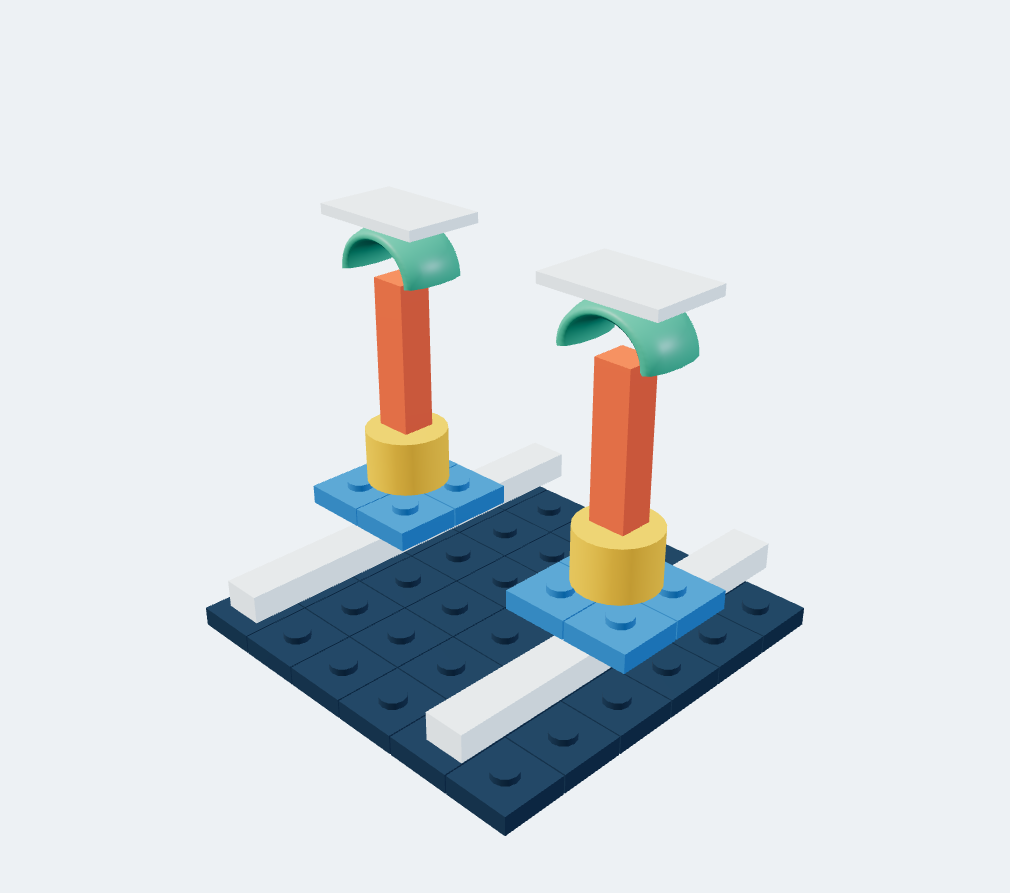
\includegraphics[width=.24\textwidth]{figures/hierarchy3/parallel-pallet-handler-iso.png}
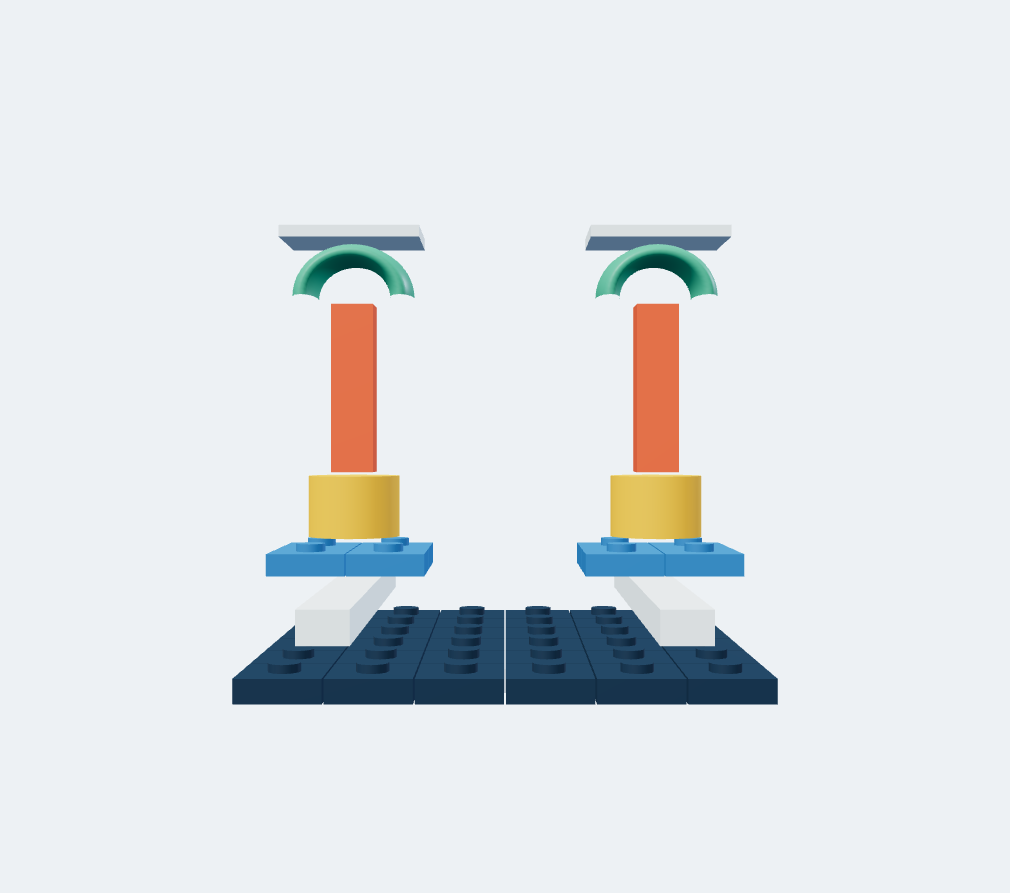
\includegraphics[width=.24\textwidth]{figures/hierarchy3/parallel-pallet-handler-front.png}
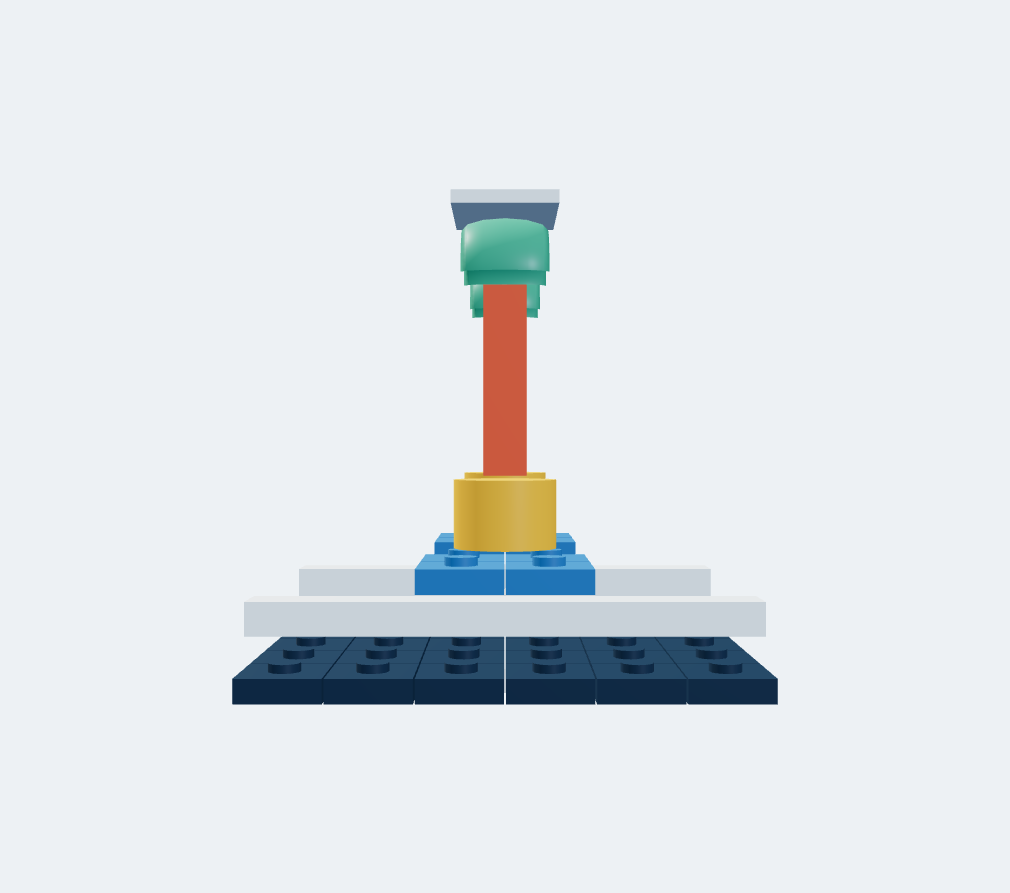
\includegraphics[width=.24\textwidth]{figures/hierarchy3/parallel-pallet-handler-side.png}
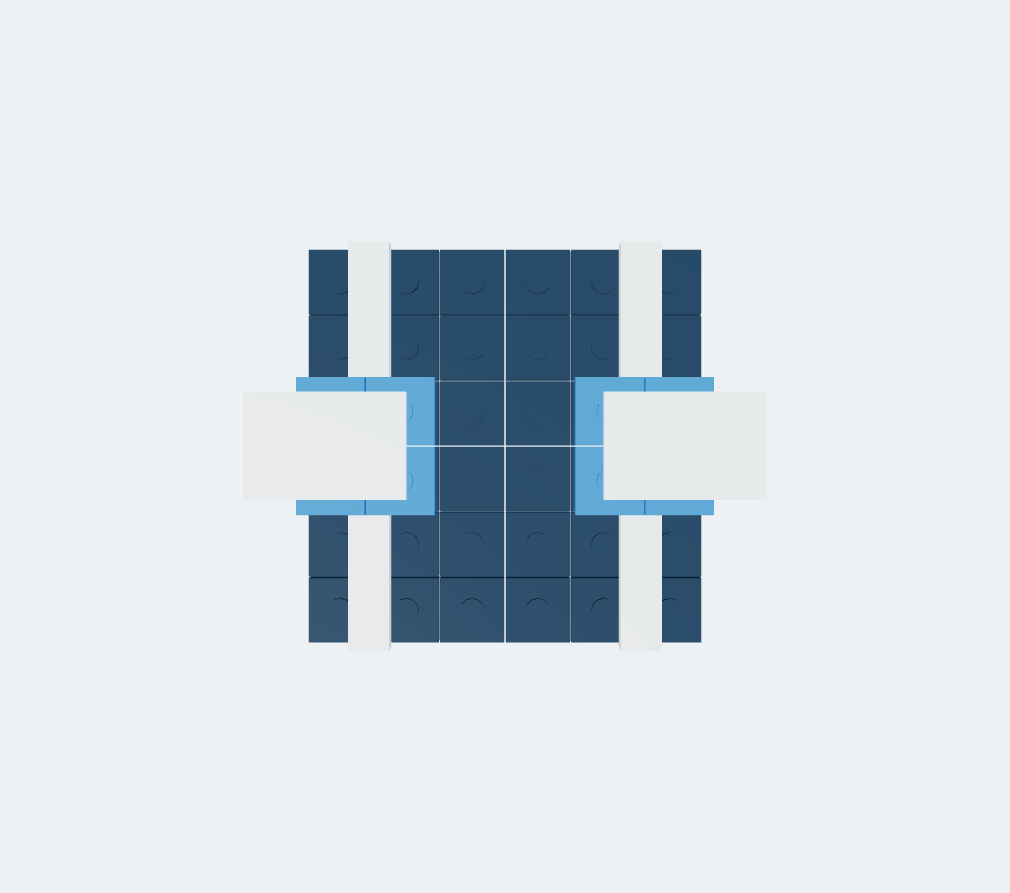
\includegraphics[width=.24\textwidth]{figures/hierarchy3/parallel-pallet-handler-top.png}
\end{center}
\noindent All 48 tasks share this source; complete inputs, choices and answers are in the companion question bank.
\begin{center}\tiny\begin{tabular}{rllll}\toprule No. & Family & Layer & Output & Evidence\\\midrule
1 & identify & atomic & single-choice & model-state \\
2 & count & atomic & single-choice & model-state \\
3 & color & atomic & single-choice & model-state \\
4 & position & atomic & single-choice & model-state \\
5 & joint-type & atomic & single-choice & model-state \\
6 & parent & atomic & single-choice & model-state \\
7 & anchor & atomic & single-choice & model-state \\
8 & degree & atomic & single-choice & model-state \\
9 & recolor & atomic & single-choice & model-state \\
10 & add & atomic & single-choice & model-state \\
11 & remove & atomic & single-choice & model-state \\
12 & replace & atomic & single-choice & model-state \\
13 & translate & atomic & single-choice & model-state \\
14 & rotate & atomic & single-choice & model-state \\
15 & next-module & atomic & single-choice & model-state \\
16 & inventory & atomic & single-choice & model-state \\
17 & boundary & atomic & single-choice & model-state \\
18 & no-op & atomic & single-choice & model-state \\
19 & prefix & metacognitive & single-choice & support-graph \\
20 & access & metacognitive & multiple-choice & Rapier \\
21 & counterfactual & metacognitive & single-choice & support-graph \\
22 & dynamic & metacognitive & single-choice & Rapier \\
23 & kinematic & metacognitive & multiple-choice & model-state \\
24 & diagnosis & metacognitive & multiple-choice & model-state \\
25 & information-gain & metacognitive & multiple-choice & finite-world \\
26 & abstention & metacognitive & single-choice & finite-world \\
27 & posterior & metacognitive & single-choice & finite-world \\
28 & pareto & metacognitive & multiple-choice & model-state \\
29 & assembly & procedural & actions & state-machine \\
30 & disassembly & procedural & actions & state-machine \\
31 & service-repair & procedural & actions & state-machine \\
32 & compound-edit & procedural & actions & state-machine \\
33 & multi-fault & integrative & actions & state-machine \\
34 & scheduling & integrative & schedule & resource-schedule \\
35 & policy & integrative & policy & finite-world \\
36 & local-frame & atomic & single-choice & model-state \\
37 & projection & atomic & single-choice & model-state \\
38 & relative-order & atomic & single-choice & model-state \\
39 & joint-axis & atomic & single-choice & model-state \\
40 & clearance-margin & metacognitive & single-choice & model-state \\
41 & load-moment & metacognitive & single-choice & model-state \\
42 & weighted-posterior & metacognitive & single-choice & finite-world \\
43 & expected-loss & metacognitive & single-choice & finite-world \\
44 & trace-threshold & metacognitive & single-choice & Rapier \\
45 & guarded-repair & procedural & actions & state-machine \\
46 & rollback & procedural & actions & state-machine \\
47 & resource-repair & integrative & actions & state-machine \\
48 & budget-policy & integrative & policy & finite-world \\
\bottomrule\end{tabular}\end{center}
\clearpage
\subsection{18. Rescue Winch Tower (D2)}
68 visible parts, 6 modules, 5 joints. Nominal representative-point displacement: 0.0530; angular displacement: 0.0065 rad. No inter-module penetration above 0.005, including directly joined modules.
\begin{center}

\includegraphics[width=.24\textwidth]{figures/hierarchy3/rescue-winch-tower-iso.png}

\includegraphics[width=.24\textwidth]{figures/hierarchy3/rescue-winch-tower-front.png}

\includegraphics[width=.24\textwidth]{figures/hierarchy3/rescue-winch-tower-side.png}

\includegraphics[width=.24\textwidth]{figures/hierarchy3/rescue-winch-tower-top.png}
\end{center}
\noindent All 48 tasks share this source; complete inputs, choices and answers are in the companion question bank.
\begin{center}\tiny\begin{tabular}{rllll}\toprule No. & Family & Layer & Output & Evidence\\\midrule
1 & identify & atomic & single-choice & model-state \\
2 & count & atomic & single-choice & model-state \\
3 & color & atomic & single-choice & model-state \\
4 & position & atomic & single-choice & model-state \\
5 & joint-type & atomic & single-choice & model-state \\
6 & parent & atomic & single-choice & model-state \\
7 & anchor & atomic & single-choice & model-state \\
8 & degree & atomic & single-choice & model-state \\
9 & recolor & atomic & single-choice & model-state \\
10 & add & atomic & single-choice & model-state \\
11 & remove & atomic & single-choice & model-state \\
12 & replace & atomic & single-choice & model-state \\
13 & translate & atomic & single-choice & model-state \\
14 & rotate & atomic & single-choice & model-state \\
15 & next-module & atomic & single-choice & model-state \\
16 & inventory & atomic & single-choice & model-state \\
17 & boundary & atomic & single-choice & model-state \\
18 & no-op & atomic & single-choice & model-state \\
19 & prefix & metacognitive & single-choice & support-graph \\
20 & access & metacognitive & multiple-choice & Rapier \\
21 & counterfactual & metacognitive & single-choice & support-graph \\
22 & dynamic & metacognitive & single-choice & Rapier \\
23 & kinematic & metacognitive & multiple-choice & model-state \\
24 & diagnosis & metacognitive & multiple-choice & model-state \\
25 & information-gain & metacognitive & multiple-choice & finite-world \\
26 & abstention & metacognitive & single-choice & finite-world \\
27 & posterior & metacognitive & single-choice & finite-world \\
28 & pareto & metacognitive & multiple-choice & model-state \\
29 & assembly & procedural & actions & state-machine \\
30 & disassembly & procedural & actions & state-machine \\
31 & service-repair & procedural & actions & state-machine \\
32 & compound-edit & procedural & actions & state-machine \\
33 & multi-fault & integrative & actions & state-machine \\
34 & scheduling & integrative & schedule & resource-schedule \\
35 & policy & integrative & policy & finite-world \\
36 & local-frame & atomic & single-choice & model-state \\
37 & projection & atomic & single-choice & model-state \\
38 & relative-order & atomic & single-choice & model-state \\
39 & joint-axis & atomic & single-choice & model-state \\
40 & clearance-margin & metacognitive & single-choice & model-state \\
41 & load-moment & metacognitive & single-choice & model-state \\
42 & weighted-posterior & metacognitive & single-choice & finite-world \\
43 & expected-loss & metacognitive & single-choice & finite-world \\
44 & trace-threshold & metacognitive & single-choice & Rapier \\
45 & guarded-repair & procedural & actions & state-machine \\
46 & rollback & procedural & actions & state-machine \\
47 & resource-repair & integrative & actions & state-machine \\
48 & budget-policy & integrative & policy & finite-world \\
\bottomrule\end{tabular}\end{center}
\clearpage
\subsection{19. Scissor Service Lift (D2)}
108 visible parts, 9 modules, 8 joints. Nominal representative-point displacement: 0.0084; angular displacement: 0.0017 rad. No inter-module penetration above 0.005, including directly joined modules.
\begin{center}

\includegraphics[width=.24\textwidth]{figures/hierarchy3/scissor-service-lift-iso.png}

\includegraphics[width=.24\textwidth]{figures/hierarchy3/scissor-service-lift-front.png}

\includegraphics[width=.24\textwidth]{figures/hierarchy3/scissor-service-lift-side.png}

\includegraphics[width=.24\textwidth]{figures/hierarchy3/scissor-service-lift-top.png}
\end{center}
\noindent All 48 tasks share this source; complete inputs, choices and answers are in the companion question bank.
\begin{center}\tiny\begin{tabular}{rllll}\toprule No. & Family & Layer & Output & Evidence\\\midrule
1 & identify & atomic & single-choice & model-state \\
2 & count & atomic & single-choice & model-state \\
3 & color & atomic & single-choice & model-state \\
4 & position & atomic & single-choice & model-state \\
5 & joint-type & atomic & single-choice & model-state \\
6 & parent & atomic & single-choice & model-state \\
7 & anchor & atomic & single-choice & model-state \\
8 & degree & atomic & single-choice & model-state \\
9 & recolor & atomic & single-choice & model-state \\
10 & add & atomic & single-choice & model-state \\
11 & remove & atomic & single-choice & model-state \\
12 & replace & atomic & single-choice & model-state \\
13 & translate & atomic & single-choice & model-state \\
14 & rotate & atomic & single-choice & model-state \\
15 & next-module & atomic & single-choice & model-state \\
16 & inventory & atomic & single-choice & model-state \\
17 & boundary & atomic & single-choice & model-state \\
18 & no-op & atomic & single-choice & model-state \\
19 & prefix & metacognitive & single-choice & support-graph \\
20 & access & metacognitive & multiple-choice & Rapier \\
21 & counterfactual & metacognitive & single-choice & support-graph \\
22 & dynamic & metacognitive & single-choice & Rapier \\
23 & kinematic & metacognitive & multiple-choice & model-state \\
24 & diagnosis & metacognitive & multiple-choice & model-state \\
25 & information-gain & metacognitive & multiple-choice & finite-world \\
26 & abstention & metacognitive & single-choice & finite-world \\
27 & posterior & metacognitive & single-choice & finite-world \\
28 & pareto & metacognitive & multiple-choice & model-state \\
29 & assembly & procedural & actions & state-machine \\
30 & disassembly & procedural & actions & state-machine \\
31 & service-repair & procedural & actions & state-machine \\
32 & compound-edit & procedural & actions & state-machine \\
33 & multi-fault & integrative & actions & state-machine \\
34 & scheduling & integrative & schedule & resource-schedule \\
35 & policy & integrative & policy & finite-world \\
36 & local-frame & atomic & single-choice & model-state \\
37 & projection & atomic & single-choice & model-state \\
38 & relative-order & atomic & single-choice & model-state \\
39 & joint-axis & atomic & single-choice & model-state \\
40 & clearance-margin & metacognitive & single-choice & model-state \\
41 & load-moment & metacognitive & single-choice & model-state \\
42 & weighted-posterior & metacognitive & single-choice & finite-world \\
43 & expected-loss & metacognitive & single-choice & finite-world \\
44 & trace-threshold & metacognitive & single-choice & Rapier \\
45 & guarded-repair & procedural & actions & state-machine \\
46 & rollback & procedural & actions & state-machine \\
47 & resource-repair & integrative & actions & state-machine \\
48 & budget-policy & integrative & policy & finite-world \\
\bottomrule\end{tabular}\end{center}
\clearpage
\subsection{20. Solar Tracker Array (D2)}
66 visible parts, 6 modules, 5 joints. Nominal representative-point displacement: 0.0000; angular displacement: 0.0000 rad. No inter-module penetration above 0.005, including directly joined modules.
\begin{center}

\includegraphics[width=.24\textwidth]{figures/hierarchy3/solar-tracker-array-iso.png}

\includegraphics[width=.24\textwidth]{figures/hierarchy3/solar-tracker-array-front.png}

\includegraphics[width=.24\textwidth]{figures/hierarchy3/solar-tracker-array-side.png}

\includegraphics[width=.24\textwidth]{figures/hierarchy3/solar-tracker-array-top.png}
\end{center}
\noindent All 48 tasks share this source; complete inputs, choices and answers are in the companion question bank.
\begin{center}\tiny\begin{tabular}{rllll}\toprule No. & Family & Layer & Output & Evidence\\\midrule
1 & identify & atomic & single-choice & model-state \\
2 & count & atomic & single-choice & model-state \\
3 & color & atomic & single-choice & model-state \\
4 & position & atomic & single-choice & model-state \\
5 & joint-type & atomic & single-choice & model-state \\
6 & parent & atomic & single-choice & model-state \\
7 & anchor & atomic & single-choice & model-state \\
8 & degree & atomic & single-choice & model-state \\
9 & recolor & atomic & single-choice & model-state \\
10 & add & atomic & single-choice & model-state \\
11 & remove & atomic & single-choice & model-state \\
12 & replace & atomic & single-choice & model-state \\
13 & translate & atomic & single-choice & model-state \\
14 & rotate & atomic & single-choice & model-state \\
15 & next-module & atomic & single-choice & model-state \\
16 & inventory & atomic & single-choice & model-state \\
17 & boundary & atomic & single-choice & model-state \\
18 & no-op & atomic & single-choice & model-state \\
19 & prefix & metacognitive & single-choice & support-graph \\
20 & access & metacognitive & multiple-choice & Rapier \\
21 & counterfactual & metacognitive & single-choice & support-graph \\
22 & dynamic & metacognitive & single-choice & Rapier \\
23 & kinematic & metacognitive & multiple-choice & model-state \\
24 & diagnosis & metacognitive & multiple-choice & model-state \\
25 & information-gain & metacognitive & multiple-choice & finite-world \\
26 & abstention & metacognitive & single-choice & finite-world \\
27 & posterior & metacognitive & single-choice & finite-world \\
28 & pareto & metacognitive & multiple-choice & model-state \\
29 & assembly & procedural & actions & state-machine \\
30 & disassembly & procedural & actions & state-machine \\
31 & service-repair & procedural & actions & state-machine \\
32 & compound-edit & procedural & actions & state-machine \\
33 & multi-fault & integrative & actions & state-machine \\
34 & scheduling & integrative & schedule & resource-schedule \\
35 & policy & integrative & policy & finite-world \\
36 & local-frame & atomic & single-choice & model-state \\
37 & projection & atomic & single-choice & model-state \\
38 & relative-order & atomic & single-choice & model-state \\
39 & joint-axis & atomic & single-choice & model-state \\
40 & clearance-margin & metacognitive & single-choice & model-state \\
41 & load-moment & metacognitive & single-choice & model-state \\
42 & weighted-posterior & metacognitive & single-choice & finite-world \\
43 & expected-loss & metacognitive & single-choice & finite-world \\
44 & trace-threshold & metacognitive & single-choice & Rapier \\
45 & guarded-repair & procedural & actions & state-machine \\
46 & rollback & procedural & actions & state-machine \\
47 & resource-repair & integrative & actions & state-machine \\
48 & budget-policy & integrative & policy & finite-world \\
\bottomrule\end{tabular}\end{center}
\clearpage
\subsection{21. Swing Loading Dock (D2)}
101 visible parts, 7 modules, 6 joints. Nominal representative-point displacement: 0.0115; angular displacement: 0.0022 rad. No inter-module penetration above 0.005, including directly joined modules.
\begin{center}

\includegraphics[width=.24\textwidth]{figures/hierarchy3/swing-dock-iso.png}

\includegraphics[width=.24\textwidth]{figures/hierarchy3/swing-dock-front.png}

\includegraphics[width=.24\textwidth]{figures/hierarchy3/swing-dock-side.png}

\includegraphics[width=.24\textwidth]{figures/hierarchy3/swing-dock-top.png}
\end{center}
\noindent All 48 tasks share this source; complete inputs, choices and answers are in the companion question bank.
\begin{center}\tiny\begin{tabular}{rllll}\toprule No. & Family & Layer & Output & Evidence\\\midrule
1 & identify & atomic & single-choice & model-state \\
2 & count & atomic & single-choice & model-state \\
3 & color & atomic & single-choice & model-state \\
4 & position & atomic & single-choice & model-state \\
5 & joint-type & atomic & single-choice & model-state \\
6 & parent & atomic & single-choice & model-state \\
7 & anchor & atomic & single-choice & model-state \\
8 & degree & atomic & single-choice & model-state \\
9 & recolor & atomic & single-choice & model-state \\
10 & add & atomic & single-choice & model-state \\
11 & remove & atomic & single-choice & model-state \\
12 & replace & atomic & single-choice & model-state \\
13 & translate & atomic & single-choice & model-state \\
14 & rotate & atomic & single-choice & model-state \\
15 & next-module & atomic & single-choice & model-state \\
16 & inventory & atomic & single-choice & model-state \\
17 & boundary & atomic & single-choice & model-state \\
18 & no-op & atomic & single-choice & model-state \\
19 & prefix & metacognitive & single-choice & support-graph \\
20 & access & metacognitive & multiple-choice & Rapier \\
21 & counterfactual & metacognitive & single-choice & support-graph \\
22 & dynamic & metacognitive & single-choice & Rapier \\
23 & kinematic & metacognitive & multiple-choice & model-state \\
24 & diagnosis & metacognitive & multiple-choice & model-state \\
25 & information-gain & metacognitive & multiple-choice & finite-world \\
26 & abstention & metacognitive & single-choice & finite-world \\
27 & posterior & metacognitive & single-choice & finite-world \\
28 & pareto & metacognitive & multiple-choice & model-state \\
29 & assembly & procedural & actions & state-machine \\
30 & disassembly & procedural & actions & state-machine \\
31 & service-repair & procedural & actions & state-machine \\
32 & compound-edit & procedural & actions & state-machine \\
33 & multi-fault & integrative & actions & state-machine \\
34 & scheduling & integrative & schedule & resource-schedule \\
35 & policy & integrative & policy & finite-world \\
36 & local-frame & atomic & single-choice & model-state \\
37 & projection & atomic & single-choice & model-state \\
38 & relative-order & atomic & single-choice & model-state \\
39 & joint-axis & atomic & single-choice & model-state \\
40 & clearance-margin & metacognitive & single-choice & model-state \\
41 & load-moment & metacognitive & single-choice & model-state \\
42 & weighted-posterior & metacognitive & single-choice & finite-world \\
43 & expected-loss & metacognitive & single-choice & finite-world \\
44 & trace-threshold & metacognitive & single-choice & Rapier \\
45 & guarded-repair & procedural & actions & state-machine \\
46 & rollback & procedural & actions & state-machine \\
47 & resource-repair & integrative & actions & state-machine \\
48 & budget-policy & integrative & policy & finite-world \\
\bottomrule\end{tabular}\end{center}
\clearpage
\subsection{22. Telescopic Optics Cart (D2)}
87 visible parts, 6 modules, 5 joints. Nominal representative-point displacement: 0.0093; angular displacement: 0.0017 rad. No inter-module penetration above 0.005, including directly joined modules.
\begin{center}

\includegraphics[width=.24\textwidth]{figures/hierarchy3/telescope-cart-iso.png}

\includegraphics[width=.24\textwidth]{figures/hierarchy3/telescope-cart-front.png}

\includegraphics[width=.24\textwidth]{figures/hierarchy3/telescope-cart-side.png}

\includegraphics[width=.24\textwidth]{figures/hierarchy3/telescope-cart-top.png}
\end{center}
\noindent All 48 tasks share this source; complete inputs, choices and answers are in the companion question bank.
\begin{center}\tiny\begin{tabular}{rllll}\toprule No. & Family & Layer & Output & Evidence\\\midrule
1 & identify & atomic & single-choice & model-state \\
2 & count & atomic & single-choice & model-state \\
3 & color & atomic & single-choice & model-state \\
4 & position & atomic & single-choice & model-state \\
5 & joint-type & atomic & single-choice & model-state \\
6 & parent & atomic & single-choice & model-state \\
7 & anchor & atomic & single-choice & model-state \\
8 & degree & atomic & single-choice & model-state \\
9 & recolor & atomic & single-choice & model-state \\
10 & add & atomic & single-choice & model-state \\
11 & remove & atomic & single-choice & model-state \\
12 & replace & atomic & single-choice & model-state \\
13 & translate & atomic & single-choice & model-state \\
14 & rotate & atomic & single-choice & model-state \\
15 & next-module & atomic & single-choice & model-state \\
16 & inventory & atomic & single-choice & model-state \\
17 & boundary & atomic & single-choice & model-state \\
18 & no-op & atomic & single-choice & model-state \\
19 & prefix & metacognitive & single-choice & support-graph \\
20 & access & metacognitive & multiple-choice & Rapier \\
21 & counterfactual & metacognitive & single-choice & support-graph \\
22 & dynamic & metacognitive & single-choice & Rapier \\
23 & kinematic & metacognitive & multiple-choice & model-state \\
24 & diagnosis & metacognitive & multiple-choice & model-state \\
25 & information-gain & metacognitive & multiple-choice & finite-world \\
26 & abstention & metacognitive & single-choice & finite-world \\
27 & posterior & metacognitive & single-choice & finite-world \\
28 & pareto & metacognitive & multiple-choice & model-state \\
29 & assembly & procedural & actions & state-machine \\
30 & disassembly & procedural & actions & state-machine \\
31 & service-repair & procedural & actions & state-machine \\
32 & compound-edit & procedural & actions & state-machine \\
33 & multi-fault & integrative & actions & state-machine \\
34 & scheduling & integrative & schedule & resource-schedule \\
35 & policy & integrative & policy & finite-world \\
36 & local-frame & atomic & single-choice & model-state \\
37 & projection & atomic & single-choice & model-state \\
38 & relative-order & atomic & single-choice & model-state \\
39 & joint-axis & atomic & single-choice & model-state \\
40 & clearance-margin & metacognitive & single-choice & model-state \\
41 & load-moment & metacognitive & single-choice & model-state \\
42 & weighted-posterior & metacognitive & single-choice & finite-world \\
43 & expected-loss & metacognitive & single-choice & finite-world \\
44 & trace-threshold & metacognitive & single-choice & Rapier \\
45 & guarded-repair & procedural & actions & state-machine \\
46 & rollback & procedural & actions & state-machine \\
47 & resource-repair & integrative & actions & state-machine \\
48 & budget-policy & integrative & policy & finite-world \\
\bottomrule\end{tabular}\end{center}
\clearpage
\subsection{23. Tracked Core Drill (D2)}
114 visible parts, 8 modules, 7 joints. Nominal representative-point displacement: 0.0159; angular displacement: 0.0026 rad. No inter-module penetration above 0.005, including directly joined modules.
\begin{center}

\includegraphics[width=.24\textwidth]{figures/hierarchy3/tracked-drill-iso.png}

\includegraphics[width=.24\textwidth]{figures/hierarchy3/tracked-drill-front.png}

\includegraphics[width=.24\textwidth]{figures/hierarchy3/tracked-drill-side.png}

\includegraphics[width=.24\textwidth]{figures/hierarchy3/tracked-drill-top.png}
\end{center}
\noindent All 48 tasks share this source; complete inputs, choices and answers are in the companion question bank.
\begin{center}\tiny\begin{tabular}{rllll}\toprule No. & Family & Layer & Output & Evidence\\\midrule
1 & identify & atomic & single-choice & model-state \\
2 & count & atomic & single-choice & model-state \\
3 & color & atomic & single-choice & model-state \\
4 & position & atomic & single-choice & model-state \\
5 & joint-type & atomic & single-choice & model-state \\
6 & parent & atomic & single-choice & model-state \\
7 & anchor & atomic & single-choice & model-state \\
8 & degree & atomic & single-choice & model-state \\
9 & recolor & atomic & single-choice & model-state \\
10 & add & atomic & single-choice & model-state \\
11 & remove & atomic & single-choice & model-state \\
12 & replace & atomic & single-choice & model-state \\
13 & translate & atomic & single-choice & model-state \\
14 & rotate & atomic & single-choice & model-state \\
15 & next-module & atomic & single-choice & model-state \\
16 & inventory & atomic & single-choice & model-state \\
17 & boundary & atomic & single-choice & model-state \\
18 & no-op & atomic & single-choice & model-state \\
19 & prefix & metacognitive & single-choice & support-graph \\
20 & access & metacognitive & multiple-choice & Rapier \\
21 & counterfactual & metacognitive & single-choice & support-graph \\
22 & dynamic & metacognitive & single-choice & Rapier \\
23 & kinematic & metacognitive & multiple-choice & model-state \\
24 & diagnosis & metacognitive & multiple-choice & model-state \\
25 & information-gain & metacognitive & multiple-choice & finite-world \\
26 & abstention & metacognitive & single-choice & finite-world \\
27 & posterior & metacognitive & single-choice & finite-world \\
28 & pareto & metacognitive & multiple-choice & model-state \\
29 & assembly & procedural & actions & state-machine \\
30 & disassembly & procedural & actions & state-machine \\
31 & service-repair & procedural & actions & state-machine \\
32 & compound-edit & procedural & actions & state-machine \\
33 & multi-fault & integrative & actions & state-machine \\
34 & scheduling & integrative & schedule & resource-schedule \\
35 & policy & integrative & policy & finite-world \\
36 & local-frame & atomic & single-choice & model-state \\
37 & projection & atomic & single-choice & model-state \\
38 & relative-order & atomic & single-choice & model-state \\
39 & joint-axis & atomic & single-choice & model-state \\
40 & clearance-margin & metacognitive & single-choice & model-state \\
41 & load-moment & metacognitive & single-choice & model-state \\
42 & weighted-posterior & metacognitive & single-choice & finite-world \\
43 & expected-loss & metacognitive & single-choice & finite-world \\
44 & trace-threshold & metacognitive & single-choice & Rapier \\
45 & guarded-repair & procedural & actions & state-machine \\
46 & rollback & procedural & actions & state-machine \\
47 & resource-repair & integrative & actions & state-machine \\
48 & budget-policy & integrative & policy & finite-world \\
\bottomrule\end{tabular}\end{center}
\clearpage
\subsection{24. Warehouse Sorter (D2)}
60 visible parts, 6 modules, 5 joints. Nominal representative-point displacement: 0.0000; angular displacement: 0.0000 rad. No inter-module penetration above 0.005, including directly joined modules.
\begin{center}

\includegraphics[width=.24\textwidth]{figures/hierarchy3/warehouse-sorter-iso.png}

\includegraphics[width=.24\textwidth]{figures/hierarchy3/warehouse-sorter-front.png}

\includegraphics[width=.24\textwidth]{figures/hierarchy3/warehouse-sorter-side.png}

\includegraphics[width=.24\textwidth]{figures/hierarchy3/warehouse-sorter-top.png}
\end{center}
\noindent All 48 tasks share this source; complete inputs, choices and answers are in the companion question bank.
\begin{center}\tiny\begin{tabular}{rllll}\toprule No. & Family & Layer & Output & Evidence\\\midrule
1 & identify & atomic & single-choice & model-state \\
2 & count & atomic & single-choice & model-state \\
3 & color & atomic & single-choice & model-state \\
4 & position & atomic & single-choice & model-state \\
5 & joint-type & atomic & single-choice & model-state \\
6 & parent & atomic & single-choice & model-state \\
7 & anchor & atomic & single-choice & model-state \\
8 & degree & atomic & single-choice & model-state \\
9 & recolor & atomic & single-choice & model-state \\
10 & add & atomic & single-choice & model-state \\
11 & remove & atomic & single-choice & model-state \\
12 & replace & atomic & single-choice & model-state \\
13 & translate & atomic & single-choice & model-state \\
14 & rotate & atomic & single-choice & model-state \\
15 & next-module & atomic & single-choice & model-state \\
16 & inventory & atomic & single-choice & model-state \\
17 & boundary & atomic & single-choice & model-state \\
18 & no-op & atomic & single-choice & model-state \\
19 & prefix & metacognitive & single-choice & support-graph \\
20 & access & metacognitive & multiple-choice & Rapier \\
21 & counterfactual & metacognitive & single-choice & support-graph \\
22 & dynamic & metacognitive & single-choice & Rapier \\
23 & kinematic & metacognitive & multiple-choice & model-state \\
24 & diagnosis & metacognitive & multiple-choice & model-state \\
25 & information-gain & metacognitive & multiple-choice & finite-world \\
26 & abstention & metacognitive & single-choice & finite-world \\
27 & posterior & metacognitive & single-choice & finite-world \\
28 & pareto & metacognitive & multiple-choice & model-state \\
29 & assembly & procedural & actions & state-machine \\
30 & disassembly & procedural & actions & state-machine \\
31 & service-repair & procedural & actions & state-machine \\
32 & compound-edit & procedural & actions & state-machine \\
33 & multi-fault & integrative & actions & state-machine \\
34 & scheduling & integrative & schedule & resource-schedule \\
35 & policy & integrative & policy & finite-world \\
36 & local-frame & atomic & single-choice & model-state \\
37 & projection & atomic & single-choice & model-state \\
38 & relative-order & atomic & single-choice & model-state \\
39 & joint-axis & atomic & single-choice & model-state \\
40 & clearance-margin & metacognitive & single-choice & model-state \\
41 & load-moment & metacognitive & single-choice & model-state \\
42 & weighted-posterior & metacognitive & single-choice & finite-world \\
43 & expected-loss & metacognitive & single-choice & finite-world \\
44 & trace-threshold & metacognitive & single-choice & Rapier \\
45 & guarded-repair & procedural & actions & state-machine \\
46 & rollback & procedural & actions & state-machine \\
47 & resource-repair & integrative & actions & state-machine \\
48 & budget-policy & integrative & policy & finite-world \\
\bottomrule\end{tabular}\end{center}
\clearpage
\subsection{25. Adaptive Radio Observatory (D3)}
92 visible parts, 4 modules, 3 joints. Nominal representative-point displacement: 0.0129; angular displacement: 0.0022 rad. No inter-module penetration above 0.005, including directly joined modules.
\begin{center}

\includegraphics[width=.24\textwidth]{figures/hierarchy3/adaptive-radio-observatory-iso.png}

\includegraphics[width=.24\textwidth]{figures/hierarchy3/adaptive-radio-observatory-front.png}

\includegraphics[width=.24\textwidth]{figures/hierarchy3/adaptive-radio-observatory-side.png}

\includegraphics[width=.24\textwidth]{figures/hierarchy3/adaptive-radio-observatory-top.png}
\end{center}
\noindent All 48 tasks share this source; complete inputs, choices and answers are in the companion question bank.
\begin{center}\tiny\begin{tabular}{rllll}\toprule No. & Family & Layer & Output & Evidence\\\midrule
1 & identify & atomic & single-choice & model-state \\
2 & count & atomic & single-choice & model-state \\
3 & color & atomic & single-choice & model-state \\
4 & position & atomic & single-choice & model-state \\
5 & joint-type & atomic & single-choice & model-state \\
6 & parent & atomic & single-choice & model-state \\
7 & anchor & atomic & single-choice & model-state \\
8 & degree & atomic & single-choice & model-state \\
9 & recolor & atomic & single-choice & model-state \\
10 & add & atomic & single-choice & model-state \\
11 & remove & atomic & single-choice & model-state \\
12 & replace & atomic & single-choice & model-state \\
13 & translate & atomic & single-choice & model-state \\
14 & rotate & atomic & single-choice & model-state \\
15 & next-module & atomic & single-choice & model-state \\
16 & inventory & atomic & single-choice & model-state \\
17 & boundary & atomic & single-choice & model-state \\
18 & no-op & atomic & single-choice & model-state \\
19 & prefix & metacognitive & single-choice & support-graph \\
20 & access & metacognitive & multiple-choice & Rapier \\
21 & counterfactual & metacognitive & single-choice & support-graph \\
22 & dynamic & metacognitive & single-choice & Rapier \\
23 & kinematic & metacognitive & multiple-choice & model-state \\
24 & diagnosis & metacognitive & multiple-choice & model-state \\
25 & information-gain & metacognitive & multiple-choice & finite-world \\
26 & abstention & metacognitive & single-choice & finite-world \\
27 & posterior & metacognitive & single-choice & finite-world \\
28 & pareto & metacognitive & multiple-choice & model-state \\
29 & assembly & procedural & actions & state-machine \\
30 & disassembly & procedural & actions & state-machine \\
31 & service-repair & procedural & actions & state-machine \\
32 & compound-edit & procedural & actions & state-machine \\
33 & multi-fault & integrative & actions & state-machine \\
34 & scheduling & integrative & schedule & resource-schedule \\
35 & policy & integrative & policy & finite-world \\
36 & local-frame & atomic & single-choice & model-state \\
37 & projection & atomic & single-choice & model-state \\
38 & relative-order & atomic & single-choice & model-state \\
39 & joint-axis & atomic & single-choice & model-state \\
40 & clearance-margin & metacognitive & single-choice & model-state \\
41 & load-moment & metacognitive & single-choice & model-state \\
42 & weighted-posterior & metacognitive & single-choice & finite-world \\
43 & expected-loss & metacognitive & single-choice & finite-world \\
44 & trace-threshold & metacognitive & single-choice & Rapier \\
45 & guarded-repair & procedural & actions & state-machine \\
46 & rollback & procedural & actions & state-machine \\
47 & resource-repair & integrative & actions & state-machine \\
48 & budget-policy & integrative & policy & finite-world \\
\bottomrule\end{tabular}\end{center}
\clearpage
\subsection{26. Bascule Canal Gate (D3)}
142 visible parts, 6 modules, 7 joints. Nominal representative-point displacement: 0.0019; angular displacement: 0.0000 rad. No inter-module penetration above 0.005, including directly joined modules.
\begin{center}

\includegraphics[width=.24\textwidth]{figures/hierarchy3/bascule-canal-gate-iso.png}

\includegraphics[width=.24\textwidth]{figures/hierarchy3/bascule-canal-gate-front.png}

\includegraphics[width=.24\textwidth]{figures/hierarchy3/bascule-canal-gate-side.png}

\includegraphics[width=.24\textwidth]{figures/hierarchy3/bascule-canal-gate-top.png}
\end{center}
\noindent All 48 tasks share this source; complete inputs, choices and answers are in the companion question bank.
\begin{center}\tiny\begin{tabular}{rllll}\toprule No. & Family & Layer & Output & Evidence\\\midrule
1 & identify & atomic & single-choice & model-state \\
2 & count & atomic & single-choice & model-state \\
3 & color & atomic & single-choice & model-state \\
4 & position & atomic & single-choice & model-state \\
5 & joint-type & atomic & single-choice & model-state \\
6 & parent & atomic & single-choice & model-state \\
7 & anchor & atomic & single-choice & model-state \\
8 & degree & atomic & single-choice & model-state \\
9 & recolor & atomic & single-choice & model-state \\
10 & add & atomic & single-choice & model-state \\
11 & remove & atomic & single-choice & model-state \\
12 & replace & atomic & single-choice & model-state \\
13 & translate & atomic & single-choice & model-state \\
14 & rotate & atomic & single-choice & model-state \\
15 & next-module & atomic & single-choice & model-state \\
16 & inventory & atomic & single-choice & model-state \\
17 & boundary & atomic & single-choice & model-state \\
18 & no-op & atomic & single-choice & model-state \\
19 & prefix & metacognitive & single-choice & support-graph \\
20 & access & metacognitive & multiple-choice & Rapier \\
21 & counterfactual & metacognitive & single-choice & support-graph \\
22 & dynamic & metacognitive & single-choice & Rapier \\
23 & kinematic & metacognitive & multiple-choice & model-state \\
24 & diagnosis & metacognitive & multiple-choice & model-state \\
25 & information-gain & metacognitive & multiple-choice & finite-world \\
26 & abstention & metacognitive & single-choice & finite-world \\
27 & posterior & metacognitive & single-choice & finite-world \\
28 & pareto & metacognitive & multiple-choice & model-state \\
29 & assembly & procedural & actions & state-machine \\
30 & disassembly & procedural & actions & state-machine \\
31 & service-repair & procedural & actions & state-machine \\
32 & compound-edit & procedural & actions & state-machine \\
33 & multi-fault & integrative & actions & state-machine \\
34 & scheduling & integrative & schedule & resource-schedule \\
35 & policy & integrative & policy & finite-world \\
36 & local-frame & atomic & single-choice & model-state \\
37 & projection & atomic & single-choice & model-state \\
38 & relative-order & atomic & single-choice & model-state \\
39 & joint-axis & atomic & single-choice & model-state \\
40 & clearance-margin & metacognitive & single-choice & model-state \\
41 & load-moment & metacognitive & single-choice & model-state \\
42 & weighted-posterior & metacognitive & single-choice & finite-world \\
43 & expected-loss & metacognitive & single-choice & finite-world \\
44 & trace-threshold & metacognitive & single-choice & Rapier \\
45 & guarded-repair & procedural & actions & state-machine \\
46 & rollback & procedural & actions & state-machine \\
47 & resource-repair & integrative & actions & state-machine \\
48 & budget-policy & integrative & policy & finite-world \\
\bottomrule\end{tabular}\end{center}
\clearpage
\subsection{27. Cable Inspection Robot (D3)}
108 visible parts, 11 modules, 10 joints. Nominal representative-point displacement: 0.0167; angular displacement: 0.0028 rad. No inter-module penetration above 0.005, including directly joined modules.
\begin{center}

\includegraphics[width=.24\textwidth]{figures/hierarchy3/cable-inspection-robot-iso.png}

\includegraphics[width=.24\textwidth]{figures/hierarchy3/cable-inspection-robot-front.png}

\includegraphics[width=.24\textwidth]{figures/hierarchy3/cable-inspection-robot-side.png}

\includegraphics[width=.24\textwidth]{figures/hierarchy3/cable-inspection-robot-top.png}
\end{center}
\noindent All 48 tasks share this source; complete inputs, choices and answers are in the companion question bank.
\begin{center}\tiny\begin{tabular}{rllll}\toprule No. & Family & Layer & Output & Evidence\\\midrule
1 & identify & atomic & single-choice & model-state \\
2 & count & atomic & single-choice & model-state \\
3 & color & atomic & single-choice & model-state \\
4 & position & atomic & single-choice & model-state \\
5 & joint-type & atomic & single-choice & model-state \\
6 & parent & atomic & single-choice & model-state \\
7 & anchor & atomic & single-choice & model-state \\
8 & degree & atomic & single-choice & model-state \\
9 & recolor & atomic & single-choice & model-state \\
10 & add & atomic & single-choice & model-state \\
11 & remove & atomic & single-choice & model-state \\
12 & replace & atomic & single-choice & model-state \\
13 & translate & atomic & single-choice & model-state \\
14 & rotate & atomic & single-choice & model-state \\
15 & next-module & atomic & single-choice & model-state \\
16 & inventory & atomic & single-choice & model-state \\
17 & boundary & atomic & single-choice & model-state \\
18 & no-op & atomic & single-choice & model-state \\
19 & prefix & metacognitive & single-choice & support-graph \\
20 & access & metacognitive & multiple-choice & Rapier \\
21 & counterfactual & metacognitive & single-choice & support-graph \\
22 & dynamic & metacognitive & single-choice & Rapier \\
23 & kinematic & metacognitive & multiple-choice & model-state \\
24 & diagnosis & metacognitive & multiple-choice & model-state \\
25 & information-gain & metacognitive & multiple-choice & finite-world \\
26 & abstention & metacognitive & single-choice & finite-world \\
27 & posterior & metacognitive & single-choice & finite-world \\
28 & pareto & metacognitive & multiple-choice & model-state \\
29 & assembly & procedural & actions & state-machine \\
30 & disassembly & procedural & actions & state-machine \\
31 & service-repair & procedural & actions & state-machine \\
32 & compound-edit & procedural & actions & state-machine \\
33 & multi-fault & integrative & actions & state-machine \\
34 & scheduling & integrative & schedule & resource-schedule \\
35 & policy & integrative & policy & finite-world \\
36 & local-frame & atomic & single-choice & model-state \\
37 & projection & atomic & single-choice & model-state \\
38 & relative-order & atomic & single-choice & model-state \\
39 & joint-axis & atomic & single-choice & model-state \\
40 & clearance-margin & metacognitive & single-choice & model-state \\
41 & load-moment & metacognitive & single-choice & model-state \\
42 & weighted-posterior & metacognitive & single-choice & finite-world \\
43 & expected-loss & metacognitive & single-choice & finite-world \\
44 & trace-threshold & metacognitive & single-choice & Rapier \\
45 & guarded-repair & procedural & actions & state-machine \\
46 & rollback & procedural & actions & state-machine \\
47 & resource-repair & integrative & actions & state-machine \\
48 & budget-policy & integrative & policy & finite-world \\
\bottomrule\end{tabular}\end{center}
\clearpage
\subsection{28. Harbor Container Crane (D3)}
126 visible parts, 5 modules, 5 joints. Nominal representative-point displacement: 0.0014; angular displacement: 0.0000 rad. No inter-module penetration above 0.005, including directly joined modules.
\begin{center}

\includegraphics[width=.24\textwidth]{figures/hierarchy3/harbor-container-crane-iso.png}

\includegraphics[width=.24\textwidth]{figures/hierarchy3/harbor-container-crane-front.png}

\includegraphics[width=.24\textwidth]{figures/hierarchy3/harbor-container-crane-side.png}

\includegraphics[width=.24\textwidth]{figures/hierarchy3/harbor-container-crane-top.png}
\end{center}
\noindent All 48 tasks share this source; complete inputs, choices and answers are in the companion question bank.
\begin{center}\tiny\begin{tabular}{rllll}\toprule No. & Family & Layer & Output & Evidence\\\midrule
1 & identify & atomic & single-choice & model-state \\
2 & count & atomic & single-choice & model-state \\
3 & color & atomic & single-choice & model-state \\
4 & position & atomic & single-choice & model-state \\
5 & joint-type & atomic & single-choice & model-state \\
6 & parent & atomic & single-choice & model-state \\
7 & anchor & atomic & single-choice & model-state \\
8 & degree & atomic & single-choice & model-state \\
9 & recolor & atomic & single-choice & model-state \\
10 & add & atomic & single-choice & model-state \\
11 & remove & atomic & single-choice & model-state \\
12 & replace & atomic & single-choice & model-state \\
13 & translate & atomic & single-choice & model-state \\
14 & rotate & atomic & single-choice & model-state \\
15 & next-module & atomic & single-choice & model-state \\
16 & inventory & atomic & single-choice & model-state \\
17 & boundary & atomic & single-choice & model-state \\
18 & no-op & atomic & single-choice & model-state \\
19 & prefix & metacognitive & single-choice & support-graph \\
20 & access & metacognitive & multiple-choice & Rapier \\
21 & counterfactual & metacognitive & single-choice & support-graph \\
22 & dynamic & metacognitive & single-choice & Rapier \\
23 & kinematic & metacognitive & multiple-choice & model-state \\
24 & diagnosis & metacognitive & multiple-choice & model-state \\
25 & information-gain & metacognitive & multiple-choice & finite-world \\
26 & abstention & metacognitive & single-choice & finite-world \\
27 & posterior & metacognitive & single-choice & finite-world \\
28 & pareto & metacognitive & multiple-choice & model-state \\
29 & assembly & procedural & actions & state-machine \\
30 & disassembly & procedural & actions & state-machine \\
31 & service-repair & procedural & actions & state-machine \\
32 & compound-edit & procedural & actions & state-machine \\
33 & multi-fault & integrative & actions & state-machine \\
34 & scheduling & integrative & schedule & resource-schedule \\
35 & policy & integrative & policy & finite-world \\
36 & local-frame & atomic & single-choice & model-state \\
37 & projection & atomic & single-choice & model-state \\
38 & relative-order & atomic & single-choice & model-state \\
39 & joint-axis & atomic & single-choice & model-state \\
40 & clearance-margin & metacognitive & single-choice & model-state \\
41 & load-moment & metacognitive & single-choice & model-state \\
42 & weighted-posterior & metacognitive & single-choice & finite-world \\
43 & expected-loss & metacognitive & single-choice & finite-world \\
44 & trace-threshold & metacognitive & single-choice & Rapier \\
45 & guarded-repair & procedural & actions & state-machine \\
46 & rollback & procedural & actions & state-machine \\
47 & resource-repair & integrative & actions & state-machine \\
48 & budget-policy & integrative & policy & finite-world \\
\bottomrule\end{tabular}\end{center}
\clearpage
\subsection{29. Orbital Service Rover (D3)}
73 visible parts, 10 modules, 9 joints. Nominal representative-point displacement: 0.0004; angular displacement: 0.0000 rad. No inter-module penetration above 0.005, including directly joined modules.
\begin{center}

\includegraphics[width=.24\textwidth]{figures/hierarchy3/orbital-service-rover-iso.png}

\includegraphics[width=.24\textwidth]{figures/hierarchy3/orbital-service-rover-front.png}

\includegraphics[width=.24\textwidth]{figures/hierarchy3/orbital-service-rover-side.png}

\includegraphics[width=.24\textwidth]{figures/hierarchy3/orbital-service-rover-top.png}
\end{center}
\noindent All 48 tasks share this source; complete inputs, choices and answers are in the companion question bank.
\begin{center}\tiny\begin{tabular}{rllll}\toprule No. & Family & Layer & Output & Evidence\\\midrule
1 & identify & atomic & single-choice & model-state \\
2 & count & atomic & single-choice & model-state \\
3 & color & atomic & single-choice & model-state \\
4 & position & atomic & single-choice & model-state \\
5 & joint-type & atomic & single-choice & model-state \\
6 & parent & atomic & single-choice & model-state \\
7 & anchor & atomic & single-choice & model-state \\
8 & degree & atomic & single-choice & model-state \\
9 & recolor & atomic & single-choice & model-state \\
10 & add & atomic & single-choice & model-state \\
11 & remove & atomic & single-choice & model-state \\
12 & replace & atomic & single-choice & model-state \\
13 & translate & atomic & single-choice & model-state \\
14 & rotate & atomic & single-choice & model-state \\
15 & next-module & atomic & single-choice & model-state \\
16 & inventory & atomic & single-choice & model-state \\
17 & boundary & atomic & single-choice & model-state \\
18 & no-op & atomic & single-choice & model-state \\
19 & prefix & metacognitive & single-choice & support-graph \\
20 & access & metacognitive & multiple-choice & Rapier \\
21 & counterfactual & metacognitive & single-choice & support-graph \\
22 & dynamic & metacognitive & single-choice & Rapier \\
23 & kinematic & metacognitive & multiple-choice & model-state \\
24 & diagnosis & metacognitive & multiple-choice & model-state \\
25 & information-gain & metacognitive & multiple-choice & finite-world \\
26 & abstention & metacognitive & single-choice & finite-world \\
27 & posterior & metacognitive & single-choice & finite-world \\
28 & pareto & metacognitive & multiple-choice & model-state \\
29 & assembly & procedural & actions & state-machine \\
30 & disassembly & procedural & actions & state-machine \\
31 & service-repair & procedural & actions & state-machine \\
32 & compound-edit & procedural & actions & state-machine \\
33 & multi-fault & integrative & actions & state-machine \\
34 & scheduling & integrative & schedule & resource-schedule \\
35 & policy & integrative & policy & finite-world \\
36 & local-frame & atomic & single-choice & model-state \\
37 & projection & atomic & single-choice & model-state \\
38 & relative-order & atomic & single-choice & model-state \\
39 & joint-axis & atomic & single-choice & model-state \\
40 & clearance-margin & metacognitive & single-choice & model-state \\
41 & load-moment & metacognitive & single-choice & model-state \\
42 & weighted-posterior & metacognitive & single-choice & finite-world \\
43 & expected-loss & metacognitive & single-choice & finite-world \\
44 & trace-threshold & metacognitive & single-choice & Rapier \\
45 & guarded-repair & procedural & actions & state-machine \\
46 & rollback & procedural & actions & state-machine \\
47 & resource-repair & integrative & actions & state-machine \\
48 & budget-policy & integrative & policy & finite-world \\
\bottomrule\end{tabular}\end{center}
\clearpage
\subsection{30. Polar Research Station (D3)}
66 visible parts, 5 modules, 4 joints. Nominal representative-point displacement: 0.0000; angular displacement: 0.0000 rad. No inter-module penetration above 0.005, including directly joined modules.
\begin{center}

\includegraphics[width=.24\textwidth]{figures/hierarchy3/polar-research-station-iso.png}

\includegraphics[width=.24\textwidth]{figures/hierarchy3/polar-research-station-front.png}

\includegraphics[width=.24\textwidth]{figures/hierarchy3/polar-research-station-side.png}

\includegraphics[width=.24\textwidth]{figures/hierarchy3/polar-research-station-top.png}
\end{center}
\noindent All 48 tasks share this source; complete inputs, choices and answers are in the companion question bank.
\begin{center}\tiny\begin{tabular}{rllll}\toprule No. & Family & Layer & Output & Evidence\\\midrule
1 & identify & atomic & single-choice & model-state \\
2 & count & atomic & single-choice & model-state \\
3 & color & atomic & single-choice & model-state \\
4 & position & atomic & single-choice & model-state \\
5 & joint-type & atomic & single-choice & model-state \\
6 & parent & atomic & single-choice & model-state \\
7 & anchor & atomic & single-choice & model-state \\
8 & degree & atomic & single-choice & model-state \\
9 & recolor & atomic & single-choice & model-state \\
10 & add & atomic & single-choice & model-state \\
11 & remove & atomic & single-choice & model-state \\
12 & replace & atomic & single-choice & model-state \\
13 & translate & atomic & single-choice & model-state \\
14 & rotate & atomic & single-choice & model-state \\
15 & next-module & atomic & single-choice & model-state \\
16 & inventory & atomic & single-choice & model-state \\
17 & boundary & atomic & single-choice & model-state \\
18 & no-op & atomic & single-choice & model-state \\
19 & prefix & metacognitive & single-choice & support-graph \\
20 & access & metacognitive & multiple-choice & Rapier \\
21 & counterfactual & metacognitive & single-choice & support-graph \\
22 & dynamic & metacognitive & single-choice & Rapier \\
23 & kinematic & metacognitive & multiple-choice & model-state \\
24 & diagnosis & metacognitive & multiple-choice & model-state \\
25 & information-gain & metacognitive & multiple-choice & finite-world \\
26 & abstention & metacognitive & single-choice & finite-world \\
27 & posterior & metacognitive & single-choice & finite-world \\
28 & pareto & metacognitive & multiple-choice & model-state \\
29 & assembly & procedural & actions & state-machine \\
30 & disassembly & procedural & actions & state-machine \\
31 & service-repair & procedural & actions & state-machine \\
32 & compound-edit & procedural & actions & state-machine \\
33 & multi-fault & integrative & actions & state-machine \\
34 & scheduling & integrative & schedule & resource-schedule \\
35 & policy & integrative & policy & finite-world \\
36 & local-frame & atomic & single-choice & model-state \\
37 & projection & atomic & single-choice & model-state \\
38 & relative-order & atomic & single-choice & model-state \\
39 & joint-axis & atomic & single-choice & model-state \\
40 & clearance-margin & metacognitive & single-choice & model-state \\
41 & load-moment & metacognitive & single-choice & model-state \\
42 & weighted-posterior & metacognitive & single-choice & finite-world \\
43 & expected-loss & metacognitive & single-choice & finite-world \\
44 & trace-threshold & metacognitive & single-choice & Rapier \\
45 & guarded-repair & procedural & actions & state-machine \\
46 & rollback & procedural & actions & state-machine \\
47 & resource-repair & integrative & actions & state-machine \\
48 & budget-policy & integrative & policy & finite-world \\
\bottomrule\end{tabular}\end{center}
\clearpage
\subsection{31. Retractable Array Radar (D3)}
140 visible parts, 10 modules, 9 joints. Nominal representative-point displacement: 0.0163; angular displacement: 0.0028 rad. No inter-module penetration above 0.005, including directly joined modules.
\begin{center}

\includegraphics[width=.24\textwidth]{figures/hierarchy3/retractable-radar-iso.png}

\includegraphics[width=.24\textwidth]{figures/hierarchy3/retractable-radar-front.png}

\includegraphics[width=.24\textwidth]{figures/hierarchy3/retractable-radar-side.png}

\includegraphics[width=.24\textwidth]{figures/hierarchy3/retractable-radar-top.png}
\end{center}
\noindent All 48 tasks share this source; complete inputs, choices and answers are in the companion question bank.
\begin{center}\tiny\begin{tabular}{rllll}\toprule No. & Family & Layer & Output & Evidence\\\midrule
1 & identify & atomic & single-choice & model-state \\
2 & count & atomic & single-choice & model-state \\
3 & color & atomic & single-choice & model-state \\
4 & position & atomic & single-choice & model-state \\
5 & joint-type & atomic & single-choice & model-state \\
6 & parent & atomic & single-choice & model-state \\
7 & anchor & atomic & single-choice & model-state \\
8 & degree & atomic & single-choice & model-state \\
9 & recolor & atomic & single-choice & model-state \\
10 & add & atomic & single-choice & model-state \\
11 & remove & atomic & single-choice & model-state \\
12 & replace & atomic & single-choice & model-state \\
13 & translate & atomic & single-choice & model-state \\
14 & rotate & atomic & single-choice & model-state \\
15 & next-module & atomic & single-choice & model-state \\
16 & inventory & atomic & single-choice & model-state \\
17 & boundary & atomic & single-choice & model-state \\
18 & no-op & atomic & single-choice & model-state \\
19 & prefix & metacognitive & single-choice & support-graph \\
20 & access & metacognitive & multiple-choice & Rapier \\
21 & counterfactual & metacognitive & single-choice & support-graph \\
22 & dynamic & metacognitive & single-choice & Rapier \\
23 & kinematic & metacognitive & multiple-choice & model-state \\
24 & diagnosis & metacognitive & multiple-choice & model-state \\
25 & information-gain & metacognitive & multiple-choice & finite-world \\
26 & abstention & metacognitive & single-choice & finite-world \\
27 & posterior & metacognitive & single-choice & finite-world \\
28 & pareto & metacognitive & multiple-choice & model-state \\
29 & assembly & procedural & actions & state-machine \\
30 & disassembly & procedural & actions & state-machine \\
31 & service-repair & procedural & actions & state-machine \\
32 & compound-edit & procedural & actions & state-machine \\
33 & multi-fault & integrative & actions & state-machine \\
34 & scheduling & integrative & schedule & resource-schedule \\
35 & policy & integrative & policy & finite-world \\
36 & local-frame & atomic & single-choice & model-state \\
37 & projection & atomic & single-choice & model-state \\
38 & relative-order & atomic & single-choice & model-state \\
39 & joint-axis & atomic & single-choice & model-state \\
40 & clearance-margin & metacognitive & single-choice & model-state \\
41 & load-moment & metacognitive & single-choice & model-state \\
42 & weighted-posterior & metacognitive & single-choice & finite-world \\
43 & expected-loss & metacognitive & single-choice & finite-world \\
44 & trace-threshold & metacognitive & single-choice & Rapier \\
45 & guarded-repair & procedural & actions & state-machine \\
46 & rollback & procedural & actions & state-machine \\
47 & resource-repair & integrative & actions & state-machine \\
48 & budget-policy & integrative & policy & finite-world \\
\bottomrule\end{tabular}\end{center}
\clearpage
\subsection{32. Rotary Bucket Excavator (D3)}
154 visible parts, 11 modules, 10 joints. Nominal representative-point displacement: 0.0144; angular displacement: 0.0022 rad. No inter-module penetration above 0.005, including directly joined modules.
\begin{center}

\includegraphics[width=.24\textwidth]{figures/hierarchy3/rotary-excavator-iso.png}

\includegraphics[width=.24\textwidth]{figures/hierarchy3/rotary-excavator-front.png}

\includegraphics[width=.24\textwidth]{figures/hierarchy3/rotary-excavator-side.png}

\includegraphics[width=.24\textwidth]{figures/hierarchy3/rotary-excavator-top.png}
\end{center}
\noindent All 48 tasks share this source; complete inputs, choices and answers are in the companion question bank.
\begin{center}\tiny\begin{tabular}{rllll}\toprule No. & Family & Layer & Output & Evidence\\\midrule
1 & identify & atomic & single-choice & model-state \\
2 & count & atomic & single-choice & model-state \\
3 & color & atomic & single-choice & model-state \\
4 & position & atomic & single-choice & model-state \\
5 & joint-type & atomic & single-choice & model-state \\
6 & parent & atomic & single-choice & model-state \\
7 & anchor & atomic & single-choice & model-state \\
8 & degree & atomic & single-choice & model-state \\
9 & recolor & atomic & single-choice & model-state \\
10 & add & atomic & single-choice & model-state \\
11 & remove & atomic & single-choice & model-state \\
12 & replace & atomic & single-choice & model-state \\
13 & translate & atomic & single-choice & model-state \\
14 & rotate & atomic & single-choice & model-state \\
15 & next-module & atomic & single-choice & model-state \\
16 & inventory & atomic & single-choice & model-state \\
17 & boundary & atomic & single-choice & model-state \\
18 & no-op & atomic & single-choice & model-state \\
19 & prefix & metacognitive & single-choice & support-graph \\
20 & access & metacognitive & multiple-choice & Rapier \\
21 & counterfactual & metacognitive & single-choice & support-graph \\
22 & dynamic & metacognitive & single-choice & Rapier \\
23 & kinematic & metacognitive & multiple-choice & model-state \\
24 & diagnosis & metacognitive & multiple-choice & model-state \\
25 & information-gain & metacognitive & multiple-choice & finite-world \\
26 & abstention & metacognitive & single-choice & finite-world \\
27 & posterior & metacognitive & single-choice & finite-world \\
28 & pareto & metacognitive & multiple-choice & model-state \\
29 & assembly & procedural & actions & state-machine \\
30 & disassembly & procedural & actions & state-machine \\
31 & service-repair & procedural & actions & state-machine \\
32 & compound-edit & procedural & actions & state-machine \\
33 & multi-fault & integrative & actions & state-machine \\
34 & scheduling & integrative & schedule & resource-schedule \\
35 & policy & integrative & policy & finite-world \\
36 & local-frame & atomic & single-choice & model-state \\
37 & projection & atomic & single-choice & model-state \\
38 & relative-order & atomic & single-choice & model-state \\
39 & joint-axis & atomic & single-choice & model-state \\
40 & clearance-margin & metacognitive & single-choice & model-state \\
41 & load-moment & metacognitive & single-choice & model-state \\
42 & weighted-posterior & metacognitive & single-choice & finite-world \\
43 & expected-loss & metacognitive & single-choice & finite-world \\
44 & trace-threshold & metacognitive & single-choice & Rapier \\
45 & guarded-repair & procedural & actions & state-machine \\
46 & rollback & procedural & actions & state-machine \\
47 & resource-repair & integrative & actions & state-machine \\
48 & budget-policy & integrative & policy & finite-world \\
\bottomrule\end{tabular}\end{center}
\clearpage
\subsection{33. Segmented Petal Observatory (D3)}
196 visible parts, 43 modules, 42 joints. Nominal representative-point displacement: 0.0000; angular displacement: 0.0000 rad. No inter-module penetration above 0.005, including directly joined modules.
\begin{center}
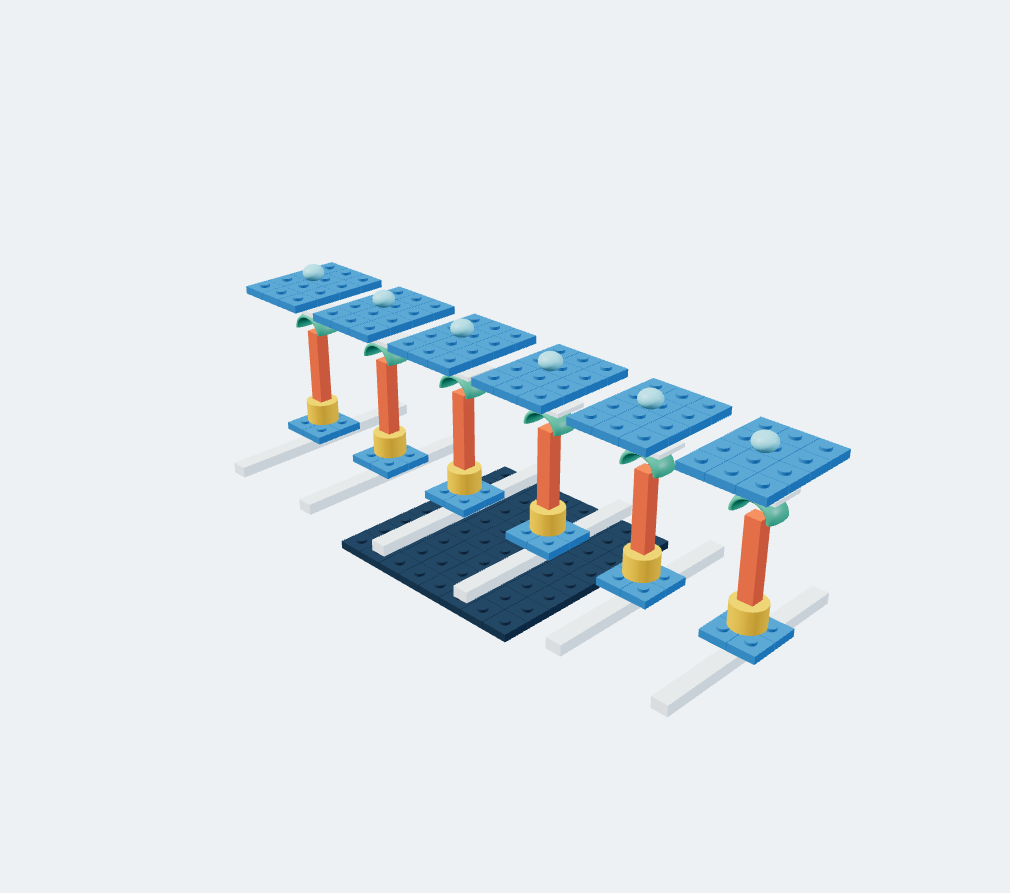
\includegraphics[width=.24\textwidth]{figures/hierarchy3/segmented-petal-observatory-iso.png}
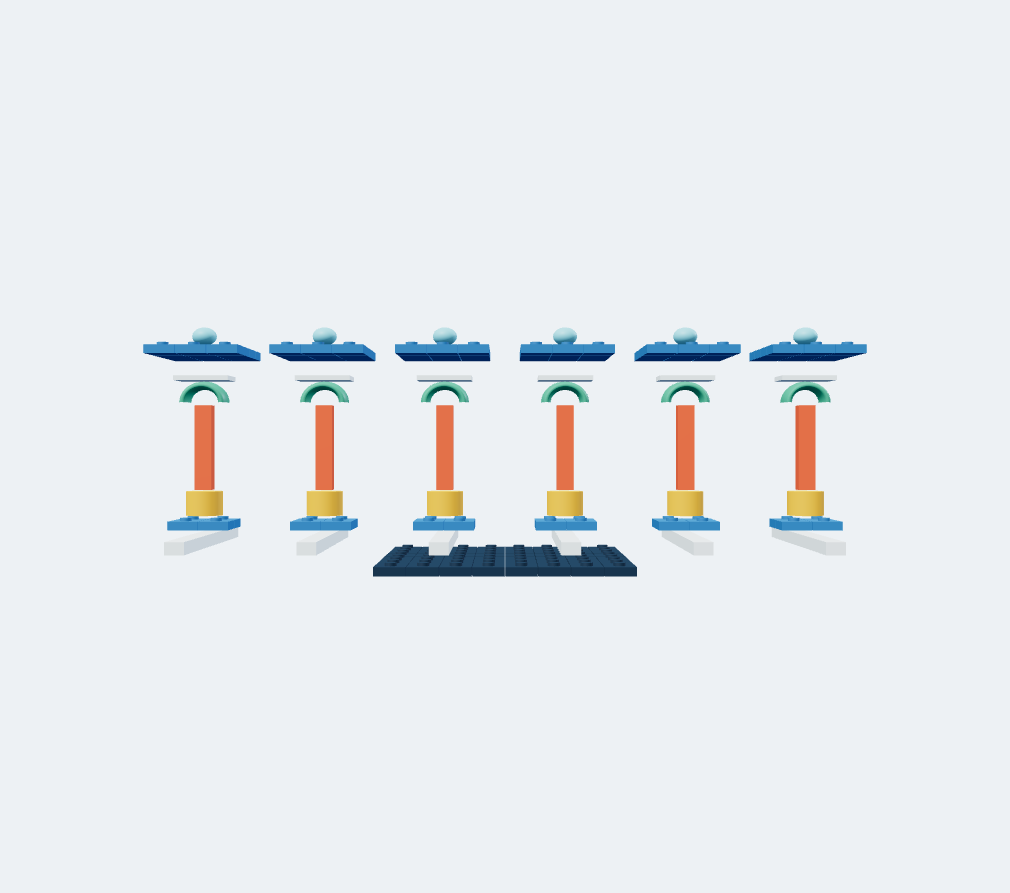
\includegraphics[width=.24\textwidth]{figures/hierarchy3/segmented-petal-observatory-front.png}
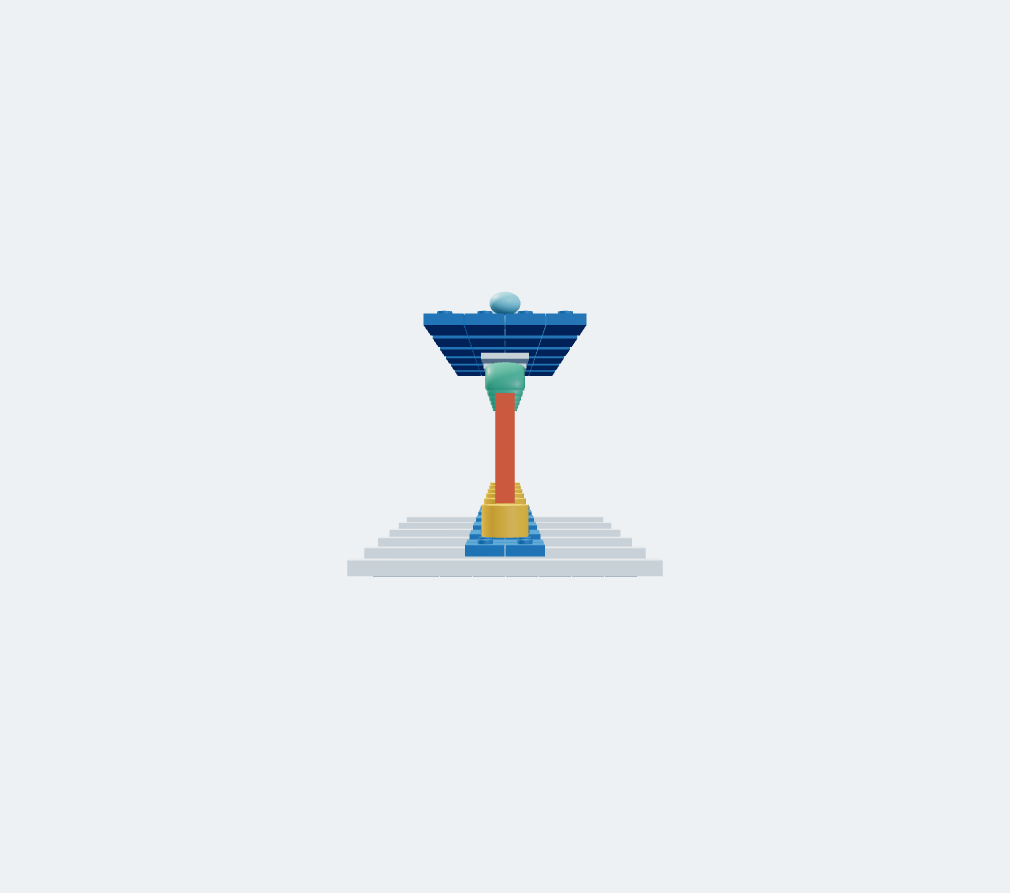
\includegraphics[width=.24\textwidth]{figures/hierarchy3/segmented-petal-observatory-side.png}
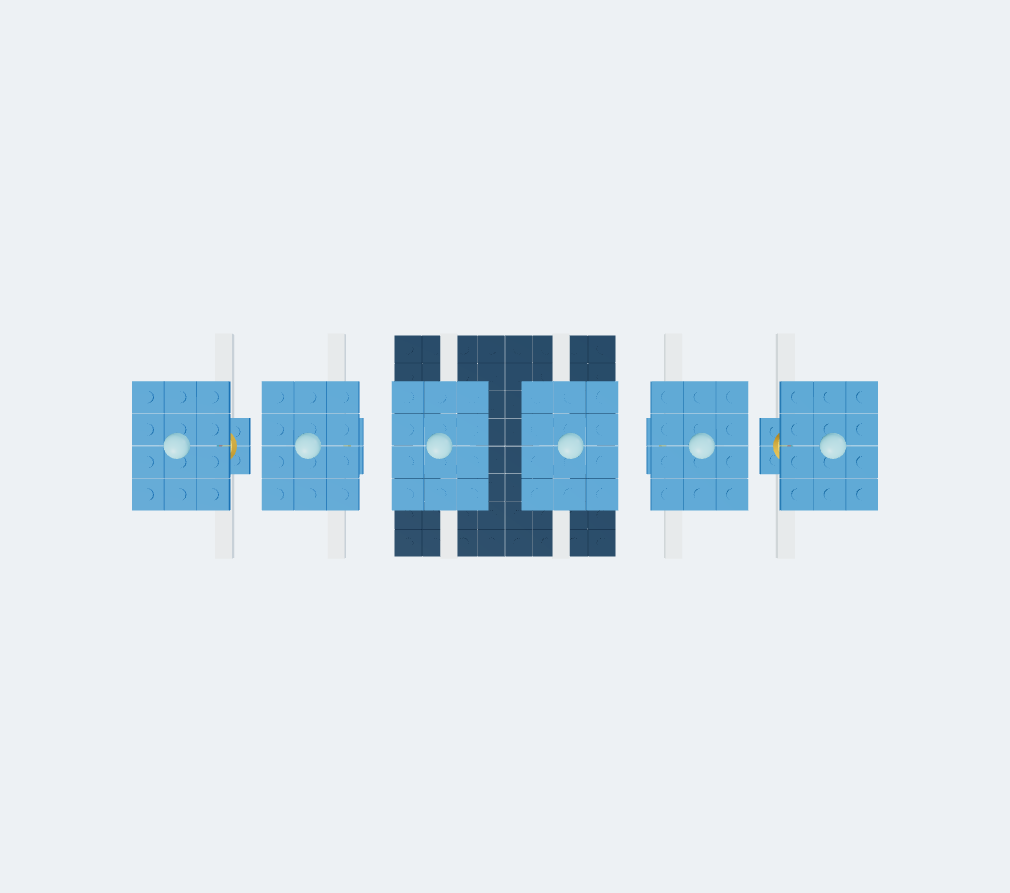
\includegraphics[width=.24\textwidth]{figures/hierarchy3/segmented-petal-observatory-top.png}
\end{center}
\noindent All 48 tasks share this source; complete inputs, choices and answers are in the companion question bank.
\begin{center}\tiny\begin{tabular}{rllll}\toprule No. & Family & Layer & Output & Evidence\\\midrule
1 & identify & atomic & single-choice & model-state \\
2 & count & atomic & single-choice & model-state \\
3 & color & atomic & single-choice & model-state \\
4 & position & atomic & single-choice & model-state \\
5 & joint-type & atomic & single-choice & model-state \\
6 & parent & atomic & single-choice & model-state \\
7 & anchor & atomic & single-choice & model-state \\
8 & degree & atomic & single-choice & model-state \\
9 & recolor & atomic & single-choice & model-state \\
10 & add & atomic & single-choice & model-state \\
11 & remove & atomic & single-choice & model-state \\
12 & replace & atomic & single-choice & model-state \\
13 & translate & atomic & single-choice & model-state \\
14 & rotate & atomic & single-choice & model-state \\
15 & next-module & atomic & single-choice & model-state \\
16 & inventory & atomic & single-choice & model-state \\
17 & boundary & atomic & single-choice & model-state \\
18 & no-op & atomic & single-choice & model-state \\
19 & prefix & metacognitive & single-choice & support-graph \\
20 & access & metacognitive & multiple-choice & Rapier \\
21 & counterfactual & metacognitive & single-choice & support-graph \\
22 & dynamic & metacognitive & single-choice & Rapier \\
23 & kinematic & metacognitive & multiple-choice & model-state \\
24 & diagnosis & metacognitive & multiple-choice & model-state \\
25 & information-gain & metacognitive & multiple-choice & finite-world \\
26 & abstention & metacognitive & single-choice & finite-world \\
27 & posterior & metacognitive & single-choice & finite-world \\
28 & pareto & metacognitive & multiple-choice & model-state \\
29 & assembly & procedural & actions & state-machine \\
30 & disassembly & procedural & actions & state-machine \\
31 & service-repair & procedural & actions & state-machine \\
32 & compound-edit & procedural & actions & state-machine \\
33 & multi-fault & integrative & actions & state-machine \\
34 & scheduling & integrative & schedule & resource-schedule \\
35 & policy & integrative & policy & finite-world \\
36 & local-frame & atomic & single-choice & model-state \\
37 & projection & atomic & single-choice & model-state \\
38 & relative-order & atomic & single-choice & model-state \\
39 & joint-axis & atomic & single-choice & model-state \\
40 & clearance-margin & metacognitive & single-choice & model-state \\
41 & load-moment & metacognitive & single-choice & model-state \\
42 & weighted-posterior & metacognitive & single-choice & finite-world \\
43 & expected-loss & metacognitive & single-choice & finite-world \\
44 & trace-threshold & metacognitive & single-choice & Rapier \\
45 & guarded-repair & procedural & actions & state-machine \\
46 & rollback & procedural & actions & state-machine \\
47 & resource-repair & integrative & actions & state-machine \\
48 & budget-policy & integrative & policy & finite-world \\
\bottomrule\end{tabular}\end{center}
\clearpage
\subsection{34. Subsea Manipulator (D3)}
116 visible parts, 11 modules, 10 joints. Nominal representative-point displacement: 0.0124; angular displacement: 0.0022 rad. No inter-module penetration above 0.005, including directly joined modules.
\begin{center}

\includegraphics[width=.24\textwidth]{figures/hierarchy3/subsea-manipulator-iso.png}

\includegraphics[width=.24\textwidth]{figures/hierarchy3/subsea-manipulator-front.png}

\includegraphics[width=.24\textwidth]{figures/hierarchy3/subsea-manipulator-side.png}

\includegraphics[width=.24\textwidth]{figures/hierarchy3/subsea-manipulator-top.png}
\end{center}
\noindent All 48 tasks share this source; complete inputs, choices and answers are in the companion question bank.
\begin{center}\tiny\begin{tabular}{rllll}\toprule No. & Family & Layer & Output & Evidence\\\midrule
1 & identify & atomic & single-choice & model-state \\
2 & count & atomic & single-choice & model-state \\
3 & color & atomic & single-choice & model-state \\
4 & position & atomic & single-choice & model-state \\
5 & joint-type & atomic & single-choice & model-state \\
6 & parent & atomic & single-choice & model-state \\
7 & anchor & atomic & single-choice & model-state \\
8 & degree & atomic & single-choice & model-state \\
9 & recolor & atomic & single-choice & model-state \\
10 & add & atomic & single-choice & model-state \\
11 & remove & atomic & single-choice & model-state \\
12 & replace & atomic & single-choice & model-state \\
13 & translate & atomic & single-choice & model-state \\
14 & rotate & atomic & single-choice & model-state \\
15 & next-module & atomic & single-choice & model-state \\
16 & inventory & atomic & single-choice & model-state \\
17 & boundary & atomic & single-choice & model-state \\
18 & no-op & atomic & single-choice & model-state \\
19 & prefix & metacognitive & single-choice & support-graph \\
20 & access & metacognitive & multiple-choice & Rapier \\
21 & counterfactual & metacognitive & single-choice & support-graph \\
22 & dynamic & metacognitive & single-choice & Rapier \\
23 & kinematic & metacognitive & multiple-choice & model-state \\
24 & diagnosis & metacognitive & multiple-choice & model-state \\
25 & information-gain & metacognitive & multiple-choice & finite-world \\
26 & abstention & metacognitive & single-choice & finite-world \\
27 & posterior & metacognitive & single-choice & finite-world \\
28 & pareto & metacognitive & multiple-choice & model-state \\
29 & assembly & procedural & actions & state-machine \\
30 & disassembly & procedural & actions & state-machine \\
31 & service-repair & procedural & actions & state-machine \\
32 & compound-edit & procedural & actions & state-machine \\
33 & multi-fault & integrative & actions & state-machine \\
34 & scheduling & integrative & schedule & resource-schedule \\
35 & policy & integrative & policy & finite-world \\
36 & local-frame & atomic & single-choice & model-state \\
37 & projection & atomic & single-choice & model-state \\
38 & relative-order & atomic & single-choice & model-state \\
39 & joint-axis & atomic & single-choice & model-state \\
40 & clearance-margin & metacognitive & single-choice & model-state \\
41 & load-moment & metacognitive & single-choice & model-state \\
42 & weighted-posterior & metacognitive & single-choice & finite-world \\
43 & expected-loss & metacognitive & single-choice & finite-world \\
44 & trace-threshold & metacognitive & single-choice & Rapier \\
45 & guarded-repair & procedural & actions & state-machine \\
46 & rollback & procedural & actions & state-machine \\
47 & resource-repair & integrative & actions & state-machine \\
48 & budget-policy & integrative & policy & finite-world \\
\bottomrule\end{tabular}\end{center}
\clearpage
\subsection{35. Tri-arm Sample Handler (D3)}
130 visible parts, 22 modules, 21 joints. Nominal representative-point displacement: 0.0000; angular displacement: 0.0000 rad. No inter-module penetration above 0.005, including directly joined modules.
\begin{center}
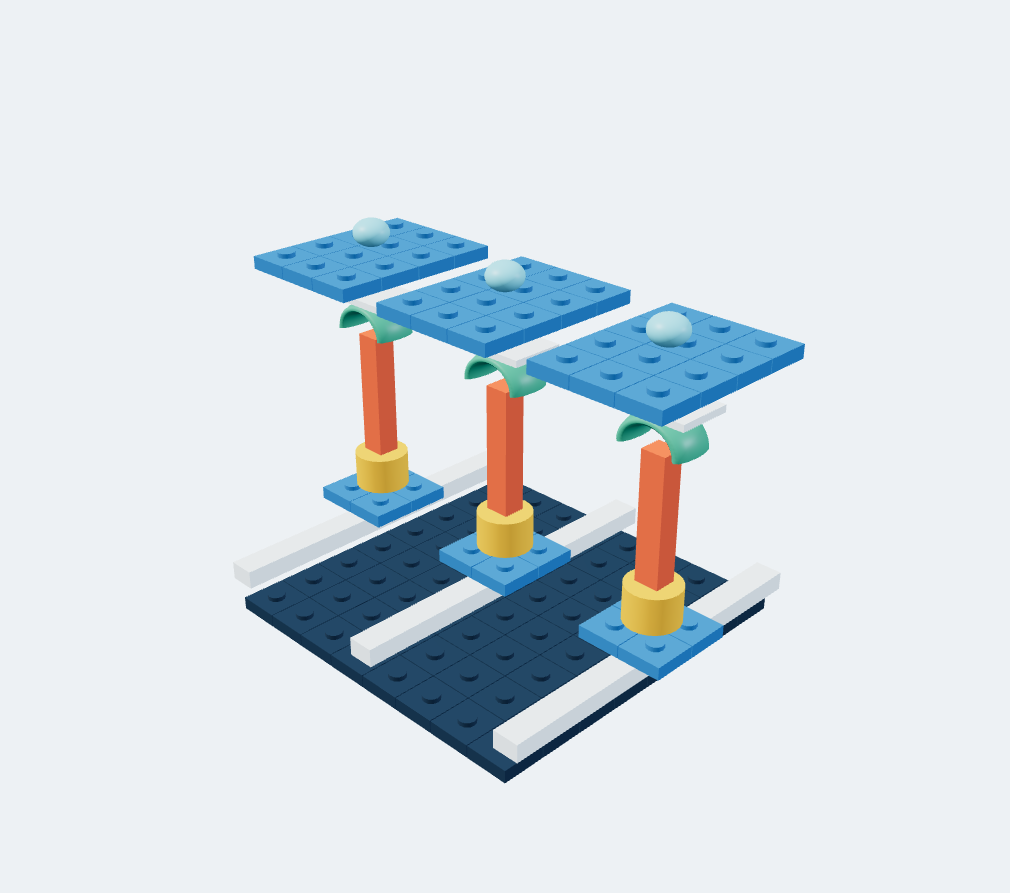
\includegraphics[width=.24\textwidth]{figures/hierarchy3/tri-arm-sample-handler-iso.png}
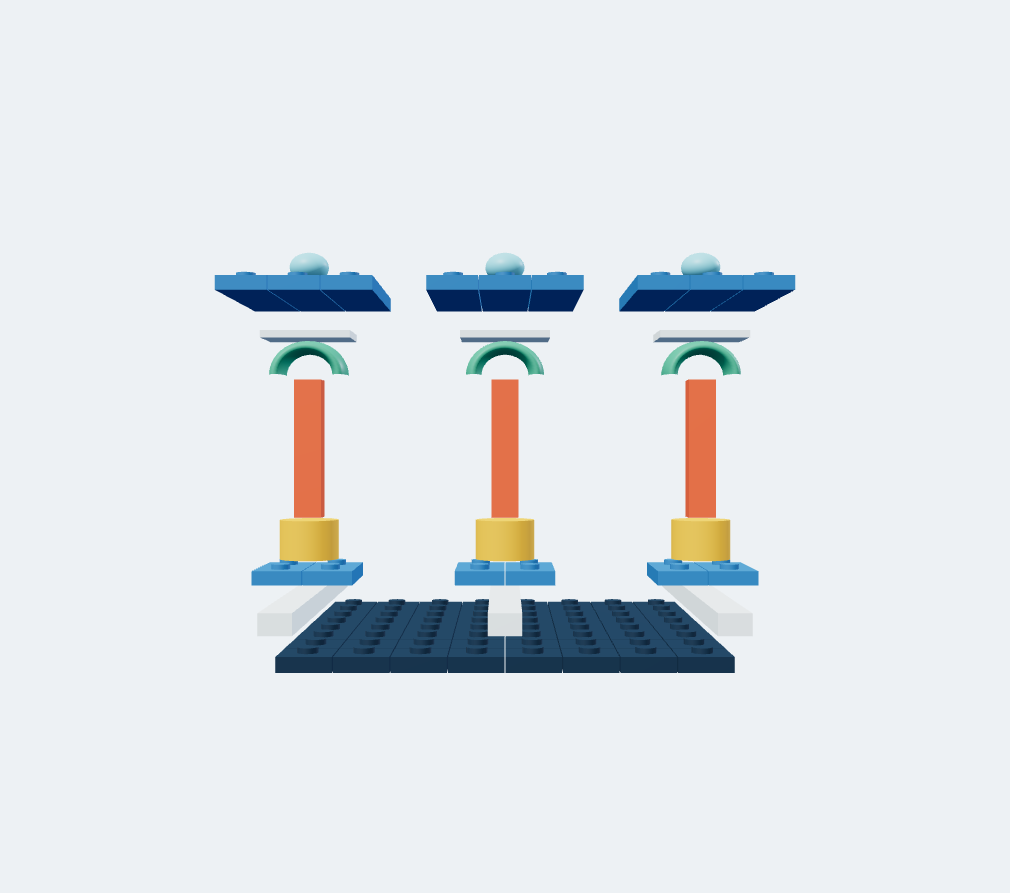
\includegraphics[width=.24\textwidth]{figures/hierarchy3/tri-arm-sample-handler-front.png}
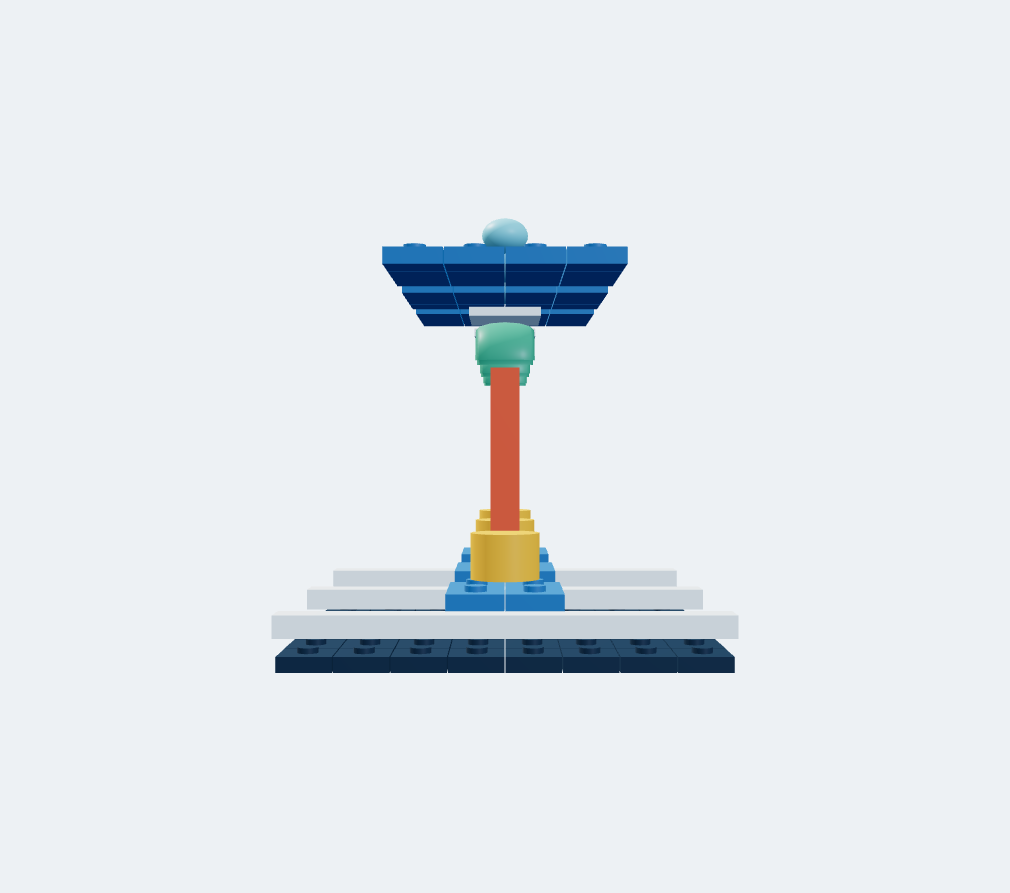
\includegraphics[width=.24\textwidth]{figures/hierarchy3/tri-arm-sample-handler-side.png}
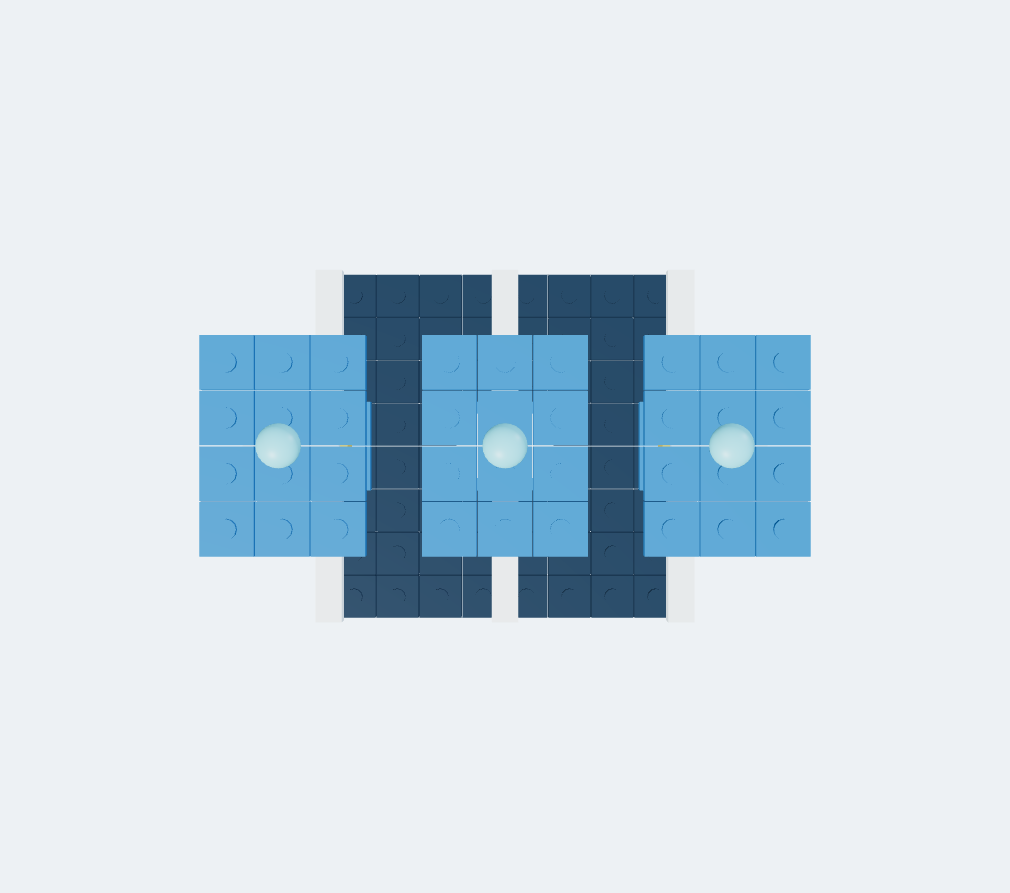
\includegraphics[width=.24\textwidth]{figures/hierarchy3/tri-arm-sample-handler-top.png}
\end{center}
\noindent All 48 tasks share this source; complete inputs, choices and answers are in the companion question bank.
\begin{center}\tiny\begin{tabular}{rllll}\toprule No. & Family & Layer & Output & Evidence\\\midrule
1 & identify & atomic & single-choice & model-state \\
2 & count & atomic & single-choice & model-state \\
3 & color & atomic & single-choice & model-state \\
4 & position & atomic & single-choice & model-state \\
5 & joint-type & atomic & single-choice & model-state \\
6 & parent & atomic & single-choice & model-state \\
7 & anchor & atomic & single-choice & model-state \\
8 & degree & atomic & single-choice & model-state \\
9 & recolor & atomic & single-choice & model-state \\
10 & add & atomic & single-choice & model-state \\
11 & remove & atomic & single-choice & model-state \\
12 & replace & atomic & single-choice & model-state \\
13 & translate & atomic & single-choice & model-state \\
14 & rotate & atomic & single-choice & model-state \\
15 & next-module & atomic & single-choice & model-state \\
16 & inventory & atomic & single-choice & model-state \\
17 & boundary & atomic & single-choice & model-state \\
18 & no-op & atomic & single-choice & model-state \\
19 & prefix & metacognitive & single-choice & support-graph \\
20 & access & metacognitive & multiple-choice & Rapier \\
21 & counterfactual & metacognitive & single-choice & support-graph \\
22 & dynamic & metacognitive & single-choice & Rapier \\
23 & kinematic & metacognitive & multiple-choice & model-state \\
24 & diagnosis & metacognitive & multiple-choice & model-state \\
25 & information-gain & metacognitive & multiple-choice & finite-world \\
26 & abstention & metacognitive & single-choice & finite-world \\
27 & posterior & metacognitive & single-choice & finite-world \\
28 & pareto & metacognitive & multiple-choice & model-state \\
29 & assembly & procedural & actions & state-machine \\
30 & disassembly & procedural & actions & state-machine \\
31 & service-repair & procedural & actions & state-machine \\
32 & compound-edit & procedural & actions & state-machine \\
33 & multi-fault & integrative & actions & state-machine \\
34 & scheduling & integrative & schedule & resource-schedule \\
35 & policy & integrative & policy & finite-world \\
36 & local-frame & atomic & single-choice & model-state \\
37 & projection & atomic & single-choice & model-state \\
38 & relative-order & atomic & single-choice & model-state \\
39 & joint-axis & atomic & single-choice & model-state \\
40 & clearance-margin & metacognitive & single-choice & model-state \\
41 & load-moment & metacognitive & single-choice & model-state \\
42 & weighted-posterior & metacognitive & single-choice & finite-world \\
43 & expected-loss & metacognitive & single-choice & finite-world \\
44 & trace-threshold & metacognitive & single-choice & Rapier \\
45 & guarded-repair & procedural & actions & state-machine \\
46 & rollback & procedural & actions & state-machine \\
47 & resource-repair & integrative & actions & state-machine \\
48 & budget-policy & integrative & policy & finite-world \\
\bottomrule\end{tabular}\end{center}
\clearpage
\subsection{36. Wildfire Tiltrotor (D3)}
43 visible parts, 6 modules, 5 joints. Nominal representative-point displacement: 0.0004; angular displacement: 0.0000 rad. No inter-module penetration above 0.005, including directly joined modules.
\begin{center}

\includegraphics[width=.24\textwidth]{figures/hierarchy3/wildfire-tiltrotor-iso.png}

\includegraphics[width=.24\textwidth]{figures/hierarchy3/wildfire-tiltrotor-front.png}

\includegraphics[width=.24\textwidth]{figures/hierarchy3/wildfire-tiltrotor-side.png}

\includegraphics[width=.24\textwidth]{figures/hierarchy3/wildfire-tiltrotor-top.png}
\end{center}
\noindent All 48 tasks share this source; complete inputs, choices and answers are in the companion question bank.
\begin{center}\tiny\begin{tabular}{rllll}\toprule No. & Family & Layer & Output & Evidence\\\midrule
1 & identify & atomic & single-choice & model-state \\
2 & count & atomic & single-choice & model-state \\
3 & color & atomic & single-choice & model-state \\
4 & position & atomic & single-choice & model-state \\
5 & joint-type & atomic & single-choice & model-state \\
6 & parent & atomic & single-choice & model-state \\
7 & anchor & atomic & single-choice & model-state \\
8 & degree & atomic & single-choice & model-state \\
9 & recolor & atomic & single-choice & model-state \\
10 & add & atomic & single-choice & model-state \\
11 & remove & atomic & single-choice & model-state \\
12 & replace & atomic & single-choice & model-state \\
13 & translate & atomic & single-choice & model-state \\
14 & rotate & atomic & single-choice & model-state \\
15 & next-module & atomic & single-choice & model-state \\
16 & inventory & atomic & single-choice & model-state \\
17 & boundary & atomic & single-choice & model-state \\
18 & no-op & atomic & single-choice & model-state \\
19 & prefix & metacognitive & single-choice & support-graph \\
20 & access & metacognitive & multiple-choice & Rapier \\
21 & counterfactual & metacognitive & single-choice & support-graph \\
22 & dynamic & metacognitive & single-choice & Rapier \\
23 & kinematic & metacognitive & multiple-choice & model-state \\
24 & diagnosis & metacognitive & multiple-choice & model-state \\
25 & information-gain & metacognitive & multiple-choice & finite-world \\
26 & abstention & metacognitive & single-choice & finite-world \\
27 & posterior & metacognitive & single-choice & finite-world \\
28 & pareto & metacognitive & multiple-choice & model-state \\
29 & assembly & procedural & actions & state-machine \\
30 & disassembly & procedural & actions & state-machine \\
31 & service-repair & procedural & actions & state-machine \\
32 & compound-edit & procedural & actions & state-machine \\
33 & multi-fault & integrative & actions & state-machine \\
34 & scheduling & integrative & schedule & resource-schedule \\
35 & policy & integrative & policy & finite-world \\
36 & local-frame & atomic & single-choice & model-state \\
37 & projection & atomic & single-choice & model-state \\
38 & relative-order & atomic & single-choice & model-state \\
39 & joint-axis & atomic & single-choice & model-state \\
40 & clearance-margin & metacognitive & single-choice & model-state \\
41 & load-moment & metacognitive & single-choice & model-state \\
42 & weighted-posterior & metacognitive & single-choice & finite-world \\
43 & expected-loss & metacognitive & single-choice & finite-world \\
44 & trace-threshold & metacognitive & single-choice & Rapier \\
45 & guarded-repair & procedural & actions & state-machine \\
46 & rollback & procedural & actions & state-machine \\
47 & resource-repair & integrative & actions & state-machine \\
48 & budget-policy & integrative & policy & finite-world \\
\bottomrule\end{tabular}\end{center}
\clearpage
\subsection{37. Aircraft Service Hangar (D4)}
437 visible parts, 22 modules, 21 joints. Nominal representative-point displacement: 0.0173; angular displacement: 0.0026 rad. No inter-module penetration above 0.005, including directly joined modules.
\begin{center}

\includegraphics[width=.24\textwidth]{figures/hierarchy3/aircraft-service-hangar-iso.png}

\includegraphics[width=.24\textwidth]{figures/hierarchy3/aircraft-service-hangar-front.png}

\includegraphics[width=.24\textwidth]{figures/hierarchy3/aircraft-service-hangar-side.png}

\includegraphics[width=.24\textwidth]{figures/hierarchy3/aircraft-service-hangar-top.png}
\end{center}
\noindent All 48 tasks share this source; complete inputs, choices and answers are in the companion question bank.
\begin{center}\tiny\begin{tabular}{rllll}\toprule No. & Family & Layer & Output & Evidence\\\midrule
1 & identify & atomic & single-choice & model-state \\
2 & count & atomic & single-choice & model-state \\
3 & color & atomic & single-choice & model-state \\
4 & position & atomic & single-choice & model-state \\
5 & joint-type & atomic & single-choice & model-state \\
6 & parent & atomic & single-choice & model-state \\
7 & anchor & atomic & single-choice & model-state \\
8 & degree & atomic & single-choice & model-state \\
9 & recolor & atomic & single-choice & model-state \\
10 & add & atomic & single-choice & model-state \\
11 & remove & atomic & single-choice & model-state \\
12 & replace & atomic & single-choice & model-state \\
13 & translate & atomic & single-choice & model-state \\
14 & rotate & atomic & single-choice & model-state \\
15 & next-module & atomic & single-choice & model-state \\
16 & inventory & atomic & single-choice & model-state \\
17 & boundary & atomic & single-choice & model-state \\
18 & no-op & atomic & single-choice & model-state \\
19 & prefix & metacognitive & single-choice & support-graph \\
20 & access & metacognitive & multiple-choice & Rapier \\
21 & counterfactual & metacognitive & single-choice & support-graph \\
22 & dynamic & metacognitive & single-choice & Rapier \\
23 & kinematic & metacognitive & multiple-choice & model-state \\
24 & diagnosis & metacognitive & multiple-choice & model-state \\
25 & information-gain & metacognitive & multiple-choice & finite-world \\
26 & abstention & metacognitive & single-choice & finite-world \\
27 & posterior & metacognitive & single-choice & finite-world \\
28 & pareto & metacognitive & multiple-choice & model-state \\
29 & assembly & procedural & actions & state-machine \\
30 & disassembly & procedural & actions & state-machine \\
31 & service-repair & procedural & actions & state-machine \\
32 & compound-edit & procedural & actions & state-machine \\
33 & multi-fault & integrative & actions & state-machine \\
34 & scheduling & integrative & schedule & resource-schedule \\
35 & policy & integrative & policy & finite-world \\
36 & local-frame & atomic & single-choice & model-state \\
37 & projection & atomic & single-choice & model-state \\
38 & relative-order & atomic & single-choice & model-state \\
39 & joint-axis & atomic & single-choice & model-state \\
40 & clearance-margin & metacognitive & single-choice & model-state \\
41 & load-moment & metacognitive & single-choice & model-state \\
42 & weighted-posterior & metacognitive & single-choice & finite-world \\
43 & expected-loss & metacognitive & single-choice & finite-world \\
44 & trace-threshold & metacognitive & single-choice & Rapier \\
45 & guarded-repair & procedural & actions & state-machine \\
46 & rollback & procedural & actions & state-machine \\
47 & resource-repair & integrative & actions & state-machine \\
48 & budget-policy & integrative & policy & finite-world \\
\bottomrule\end{tabular}\end{center}
\clearpage
\subsection{38. Automated Cargo Terminal (D4)}
231 visible parts, 13 modules, 12 joints. Nominal representative-point displacement: 0.0006; angular displacement: 0.0000 rad. No inter-module penetration above 0.005, including directly joined modules.
\begin{center}

\includegraphics[width=.24\textwidth]{figures/hierarchy3/automated-cargo-terminal-iso.png}

\includegraphics[width=.24\textwidth]{figures/hierarchy3/automated-cargo-terminal-front.png}

\includegraphics[width=.24\textwidth]{figures/hierarchy3/automated-cargo-terminal-side.png}

\includegraphics[width=.24\textwidth]{figures/hierarchy3/automated-cargo-terminal-top.png}
\end{center}
\noindent All 48 tasks share this source; complete inputs, choices and answers are in the companion question bank.
\begin{center}\tiny\begin{tabular}{rllll}\toprule No. & Family & Layer & Output & Evidence\\\midrule
1 & identify & atomic & single-choice & model-state \\
2 & count & atomic & single-choice & model-state \\
3 & color & atomic & single-choice & model-state \\
4 & position & atomic & single-choice & model-state \\
5 & joint-type & atomic & single-choice & model-state \\
6 & parent & atomic & single-choice & model-state \\
7 & anchor & atomic & single-choice & model-state \\
8 & degree & atomic & single-choice & model-state \\
9 & recolor & atomic & single-choice & model-state \\
10 & add & atomic & single-choice & model-state \\
11 & remove & atomic & single-choice & model-state \\
12 & replace & atomic & single-choice & model-state \\
13 & translate & atomic & single-choice & model-state \\
14 & rotate & atomic & single-choice & model-state \\
15 & next-module & atomic & single-choice & model-state \\
16 & inventory & atomic & single-choice & model-state \\
17 & boundary & atomic & single-choice & model-state \\
18 & no-op & atomic & single-choice & model-state \\
19 & prefix & metacognitive & single-choice & support-graph \\
20 & access & metacognitive & multiple-choice & Rapier \\
21 & counterfactual & metacognitive & single-choice & support-graph \\
22 & dynamic & metacognitive & single-choice & Rapier \\
23 & kinematic & metacognitive & multiple-choice & model-state \\
24 & diagnosis & metacognitive & multiple-choice & model-state \\
25 & information-gain & metacognitive & multiple-choice & finite-world \\
26 & abstention & metacognitive & single-choice & finite-world \\
27 & posterior & metacognitive & single-choice & finite-world \\
28 & pareto & metacognitive & multiple-choice & model-state \\
29 & assembly & procedural & actions & state-machine \\
30 & disassembly & procedural & actions & state-machine \\
31 & service-repair & procedural & actions & state-machine \\
32 & compound-edit & procedural & actions & state-machine \\
33 & multi-fault & integrative & actions & state-machine \\
34 & scheduling & integrative & schedule & resource-schedule \\
35 & policy & integrative & policy & finite-world \\
36 & local-frame & atomic & single-choice & model-state \\
37 & projection & atomic & single-choice & model-state \\
38 & relative-order & atomic & single-choice & model-state \\
39 & joint-axis & atomic & single-choice & model-state \\
40 & clearance-margin & metacognitive & single-choice & model-state \\
41 & load-moment & metacognitive & single-choice & model-state \\
42 & weighted-posterior & metacognitive & single-choice & finite-world \\
43 & expected-loss & metacognitive & single-choice & finite-world \\
44 & trace-threshold & metacognitive & single-choice & Rapier \\
45 & guarded-repair & procedural & actions & state-machine \\
46 & rollback & procedural & actions & state-machine \\
47 & resource-repair & integrative & actions & state-machine \\
48 & budget-policy & integrative & policy & finite-world \\
\bottomrule\end{tabular}\end{center}
\clearpage
\subsection{39. Automated Recycling Plant (D4)}
404 visible parts, 24 modules, 23 joints. Nominal representative-point displacement: 0.0173; angular displacement: 0.0026 rad. No inter-module penetration above 0.005, including directly joined modules.
\begin{center}

\includegraphics[width=.24\textwidth]{figures/hierarchy3/automated-recycling-plant-iso.png}

\includegraphics[width=.24\textwidth]{figures/hierarchy3/automated-recycling-plant-front.png}

\includegraphics[width=.24\textwidth]{figures/hierarchy3/automated-recycling-plant-side.png}

\includegraphics[width=.24\textwidth]{figures/hierarchy3/automated-recycling-plant-top.png}
\end{center}
\noindent All 48 tasks share this source; complete inputs, choices and answers are in the companion question bank.
\begin{center}\tiny\begin{tabular}{rllll}\toprule No. & Family & Layer & Output & Evidence\\\midrule
1 & identify & atomic & single-choice & model-state \\
2 & count & atomic & single-choice & model-state \\
3 & color & atomic & single-choice & model-state \\
4 & position & atomic & single-choice & model-state \\
5 & joint-type & atomic & single-choice & model-state \\
6 & parent & atomic & single-choice & model-state \\
7 & anchor & atomic & single-choice & model-state \\
8 & degree & atomic & single-choice & model-state \\
9 & recolor & atomic & single-choice & model-state \\
10 & add & atomic & single-choice & model-state \\
11 & remove & atomic & single-choice & model-state \\
12 & replace & atomic & single-choice & model-state \\
13 & translate & atomic & single-choice & model-state \\
14 & rotate & atomic & single-choice & model-state \\
15 & next-module & atomic & single-choice & model-state \\
16 & inventory & atomic & single-choice & model-state \\
17 & boundary & atomic & single-choice & model-state \\
18 & no-op & atomic & single-choice & model-state \\
19 & prefix & metacognitive & single-choice & support-graph \\
20 & access & metacognitive & multiple-choice & Rapier \\
21 & counterfactual & metacognitive & single-choice & support-graph \\
22 & dynamic & metacognitive & single-choice & Rapier \\
23 & kinematic & metacognitive & multiple-choice & model-state \\
24 & diagnosis & metacognitive & multiple-choice & model-state \\
25 & information-gain & metacognitive & multiple-choice & finite-world \\
26 & abstention & metacognitive & single-choice & finite-world \\
27 & posterior & metacognitive & single-choice & finite-world \\
28 & pareto & metacognitive & multiple-choice & model-state \\
29 & assembly & procedural & actions & state-machine \\
30 & disassembly & procedural & actions & state-machine \\
31 & service-repair & procedural & actions & state-machine \\
32 & compound-edit & procedural & actions & state-machine \\
33 & multi-fault & integrative & actions & state-machine \\
34 & scheduling & integrative & schedule & resource-schedule \\
35 & policy & integrative & policy & finite-world \\
36 & local-frame & atomic & single-choice & model-state \\
37 & projection & atomic & single-choice & model-state \\
38 & relative-order & atomic & single-choice & model-state \\
39 & joint-axis & atomic & single-choice & model-state \\
40 & clearance-margin & metacognitive & single-choice & model-state \\
41 & load-moment & metacognitive & single-choice & model-state \\
42 & weighted-posterior & metacognitive & single-choice & finite-world \\
43 & expected-loss & metacognitive & single-choice & finite-world \\
44 & trace-threshold & metacognitive & single-choice & Rapier \\
45 & guarded-repair & procedural & actions & state-machine \\
46 & rollback & procedural & actions & state-machine \\
47 & resource-repair & integrative & actions & state-machine \\
48 & budget-policy & integrative & policy & finite-world \\
\bottomrule\end{tabular}\end{center}
\clearpage
\subsection{40. Distributed Battery Exchange (D4)}
360 visible parts, 41 modules, 40 joints. Nominal representative-point displacement: 0.0000; angular displacement: 0.0000 rad. No inter-module penetration above 0.005, including directly joined modules.
\begin{center}
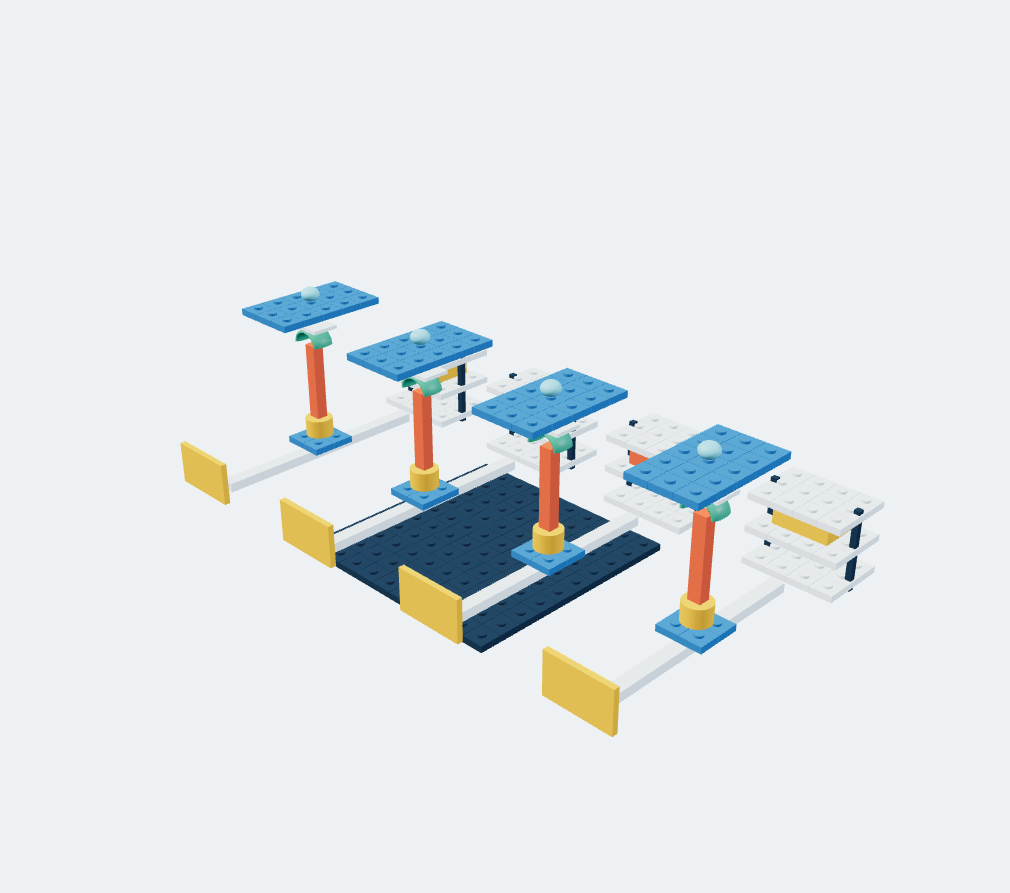
\includegraphics[width=.24\textwidth]{figures/hierarchy3/distributed-battery-exchange-iso.png}
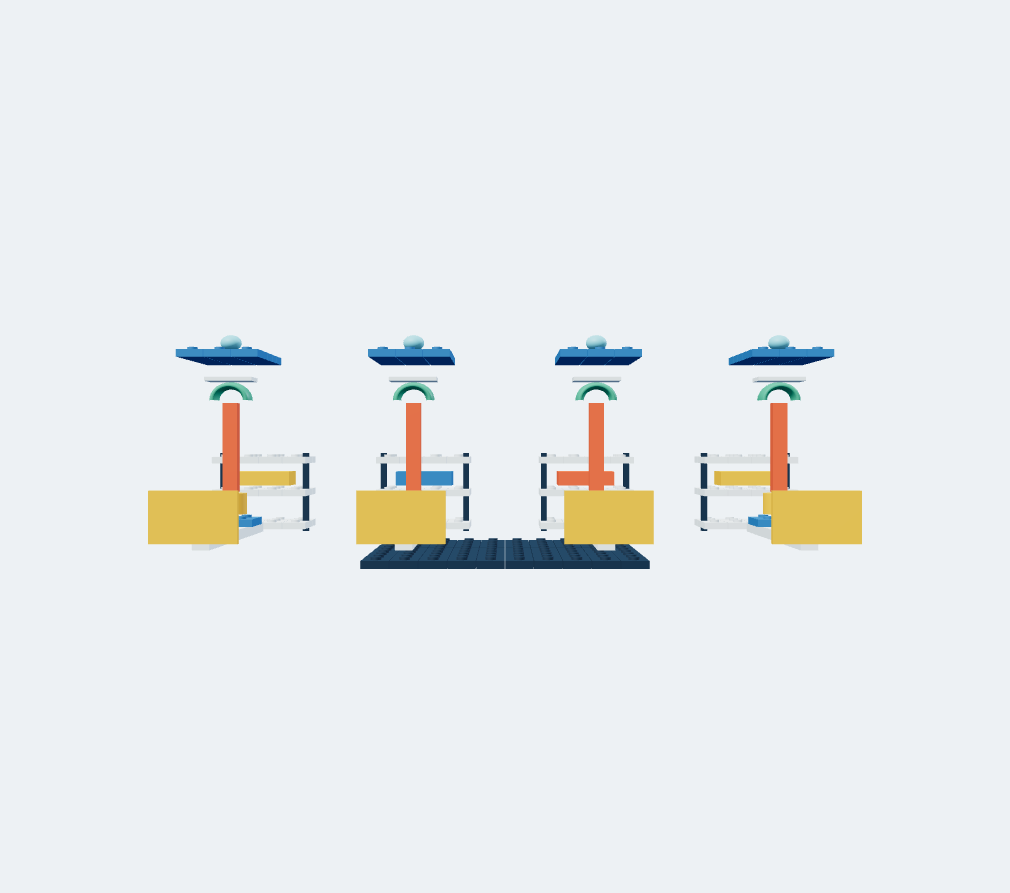
\includegraphics[width=.24\textwidth]{figures/hierarchy3/distributed-battery-exchange-front.png}
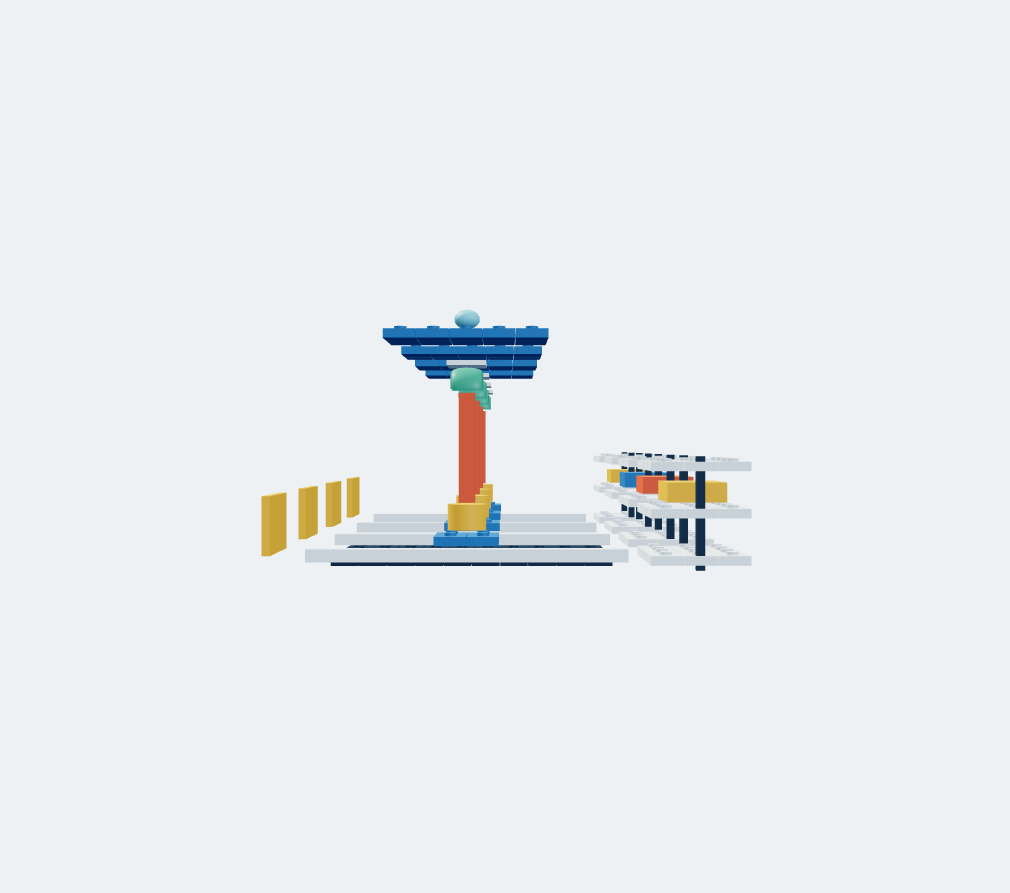
\includegraphics[width=.24\textwidth]{figures/hierarchy3/distributed-battery-exchange-side.png}
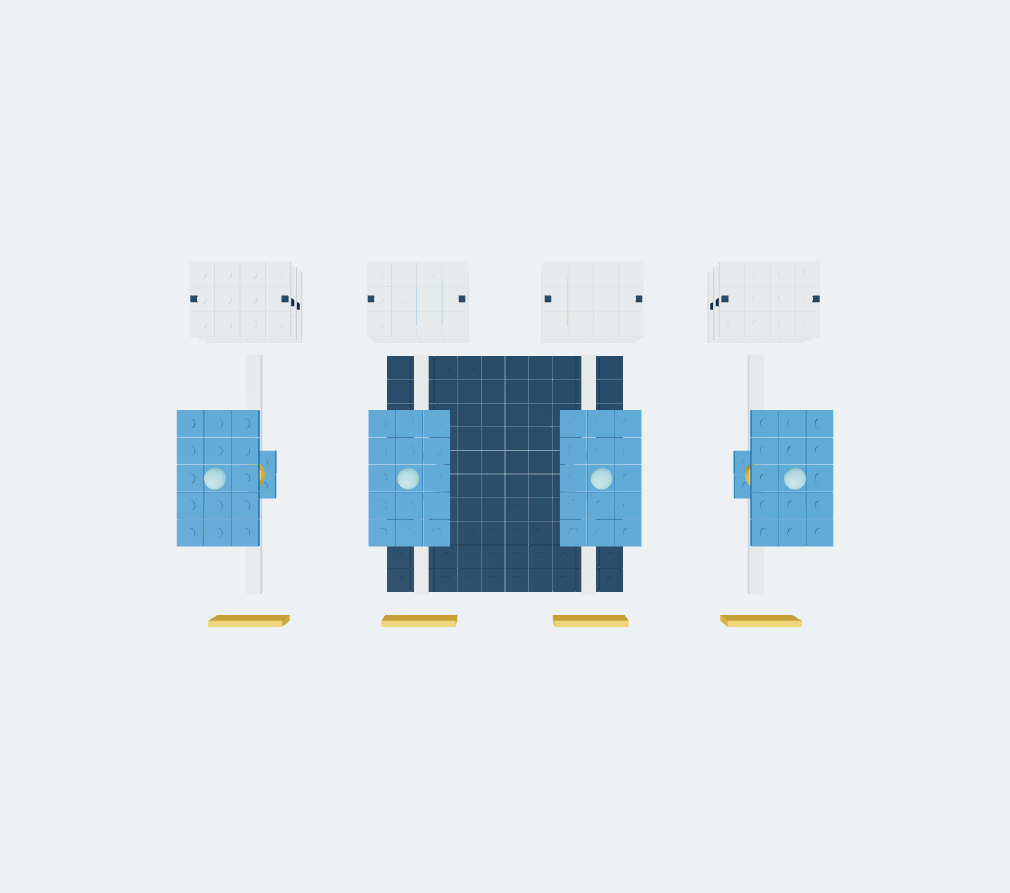
\includegraphics[width=.24\textwidth]{figures/hierarchy3/distributed-battery-exchange-top.png}
\end{center}
\noindent All 48 tasks share this source; complete inputs, choices and answers are in the companion question bank.
\begin{center}\tiny\begin{tabular}{rllll}\toprule No. & Family & Layer & Output & Evidence\\\midrule
1 & identify & atomic & single-choice & model-state \\
2 & count & atomic & single-choice & model-state \\
3 & color & atomic & single-choice & model-state \\
4 & position & atomic & single-choice & model-state \\
5 & joint-type & atomic & single-choice & model-state \\
6 & parent & atomic & single-choice & model-state \\
7 & anchor & atomic & single-choice & model-state \\
8 & degree & atomic & single-choice & model-state \\
9 & recolor & atomic & single-choice & model-state \\
10 & add & atomic & single-choice & model-state \\
11 & remove & atomic & single-choice & model-state \\
12 & replace & atomic & single-choice & model-state \\
13 & translate & atomic & single-choice & model-state \\
14 & rotate & atomic & single-choice & model-state \\
15 & next-module & atomic & single-choice & model-state \\
16 & inventory & atomic & single-choice & model-state \\
17 & boundary & atomic & single-choice & model-state \\
18 & no-op & atomic & single-choice & model-state \\
19 & prefix & metacognitive & single-choice & support-graph \\
20 & access & metacognitive & multiple-choice & Rapier \\
21 & counterfactual & metacognitive & single-choice & support-graph \\
22 & dynamic & metacognitive & single-choice & Rapier \\
23 & kinematic & metacognitive & multiple-choice & model-state \\
24 & diagnosis & metacognitive & multiple-choice & model-state \\
25 & information-gain & metacognitive & multiple-choice & finite-world \\
26 & abstention & metacognitive & single-choice & finite-world \\
27 & posterior & metacognitive & single-choice & finite-world \\
28 & pareto & metacognitive & multiple-choice & model-state \\
29 & assembly & procedural & actions & state-machine \\
30 & disassembly & procedural & actions & state-machine \\
31 & service-repair & procedural & actions & state-machine \\
32 & compound-edit & procedural & actions & state-machine \\
33 & multi-fault & integrative & actions & state-machine \\
34 & scheduling & integrative & schedule & resource-schedule \\
35 & policy & integrative & policy & finite-world \\
36 & local-frame & atomic & single-choice & model-state \\
37 & projection & atomic & single-choice & model-state \\
38 & relative-order & atomic & single-choice & model-state \\
39 & joint-axis & atomic & single-choice & model-state \\
40 & clearance-margin & metacognitive & single-choice & model-state \\
41 & load-moment & metacognitive & single-choice & model-state \\
42 & weighted-posterior & metacognitive & single-choice & finite-world \\
43 & expected-loss & metacognitive & single-choice & finite-world \\
44 & trace-threshold & metacognitive & single-choice & Rapier \\
45 & guarded-repair & procedural & actions & state-machine \\
46 & rollback & procedural & actions & state-machine \\
47 & resource-repair & integrative & actions & state-machine \\
48 & budget-policy & integrative & policy & finite-world \\
\bottomrule\end{tabular}\end{center}
\clearpage
\subsection{41. Flood Response Lock (D4)}
214 visible parts, 11 modules, 12 joints. Nominal representative-point displacement: 0.0090; angular displacement: 0.0182 rad. No inter-module penetration above 0.005, including directly joined modules.
\begin{center}

\includegraphics[width=.24\textwidth]{figures/hierarchy3/flood-response-lock-iso.png}

\includegraphics[width=.24\textwidth]{figures/hierarchy3/flood-response-lock-front.png}

\includegraphics[width=.24\textwidth]{figures/hierarchy3/flood-response-lock-side.png}

\includegraphics[width=.24\textwidth]{figures/hierarchy3/flood-response-lock-top.png}
\end{center}
\noindent All 48 tasks share this source; complete inputs, choices and answers are in the companion question bank.
\begin{center}\tiny\begin{tabular}{rllll}\toprule No. & Family & Layer & Output & Evidence\\\midrule
1 & identify & atomic & single-choice & model-state \\
2 & count & atomic & single-choice & model-state \\
3 & color & atomic & single-choice & model-state \\
4 & position & atomic & single-choice & model-state \\
5 & joint-type & atomic & single-choice & model-state \\
6 & parent & atomic & single-choice & model-state \\
7 & anchor & atomic & single-choice & model-state \\
8 & degree & atomic & single-choice & model-state \\
9 & recolor & atomic & single-choice & model-state \\
10 & add & atomic & single-choice & model-state \\
11 & remove & atomic & single-choice & model-state \\
12 & replace & atomic & single-choice & model-state \\
13 & translate & atomic & single-choice & model-state \\
14 & rotate & atomic & single-choice & model-state \\
15 & next-module & atomic & single-choice & model-state \\
16 & inventory & atomic & single-choice & model-state \\
17 & boundary & atomic & single-choice & model-state \\
18 & no-op & atomic & single-choice & model-state \\
19 & prefix & metacognitive & single-choice & support-graph \\
20 & access & metacognitive & multiple-choice & Rapier \\
21 & counterfactual & metacognitive & single-choice & support-graph \\
22 & dynamic & metacognitive & single-choice & Rapier \\
23 & kinematic & metacognitive & multiple-choice & model-state \\
24 & diagnosis & metacognitive & multiple-choice & model-state \\
25 & information-gain & metacognitive & multiple-choice & finite-world \\
26 & abstention & metacognitive & single-choice & finite-world \\
27 & posterior & metacognitive & single-choice & finite-world \\
28 & pareto & metacognitive & multiple-choice & model-state \\
29 & assembly & procedural & actions & state-machine \\
30 & disassembly & procedural & actions & state-machine \\
31 & service-repair & procedural & actions & state-machine \\
32 & compound-edit & procedural & actions & state-machine \\
33 & multi-fault & integrative & actions & state-machine \\
34 & scheduling & integrative & schedule & resource-schedule \\
35 & policy & integrative & policy & finite-world \\
36 & local-frame & atomic & single-choice & model-state \\
37 & projection & atomic & single-choice & model-state \\
38 & relative-order & atomic & single-choice & model-state \\
39 & joint-axis & atomic & single-choice & model-state \\
40 & clearance-margin & metacognitive & single-choice & model-state \\
41 & load-moment & metacognitive & single-choice & model-state \\
42 & weighted-posterior & metacognitive & single-choice & finite-world \\
43 & expected-loss & metacognitive & single-choice & finite-world \\
44 & trace-threshold & metacognitive & single-choice & Rapier \\
45 & guarded-repair & procedural & actions & state-machine \\
46 & rollback & procedural & actions & state-machine \\
47 & resource-repair & integrative & actions & state-machine \\
48 & budget-policy & integrative & policy & finite-world \\
\bottomrule\end{tabular}\end{center}
\clearpage
\subsection{42. Lunar Sample Refinery (D4)}
218 visible parts, 12 modules, 11 joints. Nominal representative-point displacement: 0.0002; angular displacement: 0.0076 rad. No inter-module penetration above 0.005, including directly joined modules.
\begin{center}

\includegraphics[width=.24\textwidth]{figures/hierarchy3/lunar-sample-refinery-iso.png}

\includegraphics[width=.24\textwidth]{figures/hierarchy3/lunar-sample-refinery-front.png}

\includegraphics[width=.24\textwidth]{figures/hierarchy3/lunar-sample-refinery-side.png}

\includegraphics[width=.24\textwidth]{figures/hierarchy3/lunar-sample-refinery-top.png}
\end{center}
\noindent All 48 tasks share this source; complete inputs, choices and answers are in the companion question bank.
\begin{center}\tiny\begin{tabular}{rllll}\toprule No. & Family & Layer & Output & Evidence\\\midrule
1 & identify & atomic & single-choice & model-state \\
2 & count & atomic & single-choice & model-state \\
3 & color & atomic & single-choice & model-state \\
4 & position & atomic & single-choice & model-state \\
5 & joint-type & atomic & single-choice & model-state \\
6 & parent & atomic & single-choice & model-state \\
7 & anchor & atomic & single-choice & model-state \\
8 & degree & atomic & single-choice & model-state \\
9 & recolor & atomic & single-choice & model-state \\
10 & add & atomic & single-choice & model-state \\
11 & remove & atomic & single-choice & model-state \\
12 & replace & atomic & single-choice & model-state \\
13 & translate & atomic & single-choice & model-state \\
14 & rotate & atomic & single-choice & model-state \\
15 & next-module & atomic & single-choice & model-state \\
16 & inventory & atomic & single-choice & model-state \\
17 & boundary & atomic & single-choice & model-state \\
18 & no-op & atomic & single-choice & model-state \\
19 & prefix & metacognitive & single-choice & support-graph \\
20 & access & metacognitive & multiple-choice & Rapier \\
21 & counterfactual & metacognitive & single-choice & support-graph \\
22 & dynamic & metacognitive & single-choice & Rapier \\
23 & kinematic & metacognitive & multiple-choice & model-state \\
24 & diagnosis & metacognitive & multiple-choice & model-state \\
25 & information-gain & metacognitive & multiple-choice & finite-world \\
26 & abstention & metacognitive & single-choice & finite-world \\
27 & posterior & metacognitive & single-choice & finite-world \\
28 & pareto & metacognitive & multiple-choice & model-state \\
29 & assembly & procedural & actions & state-machine \\
30 & disassembly & procedural & actions & state-machine \\
31 & service-repair & procedural & actions & state-machine \\
32 & compound-edit & procedural & actions & state-machine \\
33 & multi-fault & integrative & actions & state-machine \\
34 & scheduling & integrative & schedule & resource-schedule \\
35 & policy & integrative & policy & finite-world \\
36 & local-frame & atomic & single-choice & model-state \\
37 & projection & atomic & single-choice & model-state \\
38 & relative-order & atomic & single-choice & model-state \\
39 & joint-axis & atomic & single-choice & model-state \\
40 & clearance-margin & metacognitive & single-choice & model-state \\
41 & load-moment & metacognitive & single-choice & model-state \\
42 & weighted-posterior & metacognitive & single-choice & finite-world \\
43 & expected-loss & metacognitive & single-choice & finite-world \\
44 & trace-threshold & metacognitive & single-choice & Rapier \\
45 & guarded-repair & procedural & actions & state-machine \\
46 & rollback & procedural & actions & state-machine \\
47 & resource-repair & integrative & actions & state-machine \\
48 & budget-policy & integrative & policy & finite-world \\
\bottomrule\end{tabular}\end{center}
\clearpage
\subsection{43. Orbital Docking Yard (D4)}
233 visible parts, 11 modules, 10 joints. Nominal representative-point displacement: 0.0051; angular displacement: 0.0020 rad. No inter-module penetration above 0.005, including directly joined modules.
\begin{center}

\includegraphics[width=.24\textwidth]{figures/hierarchy3/orbital-docking-yard-iso.png}

\includegraphics[width=.24\textwidth]{figures/hierarchy3/orbital-docking-yard-front.png}

\includegraphics[width=.24\textwidth]{figures/hierarchy3/orbital-docking-yard-side.png}

\includegraphics[width=.24\textwidth]{figures/hierarchy3/orbital-docking-yard-top.png}
\end{center}
\noindent All 48 tasks share this source; complete inputs, choices and answers are in the companion question bank.
\begin{center}\tiny\begin{tabular}{rllll}\toprule No. & Family & Layer & Output & Evidence\\\midrule
1 & identify & atomic & single-choice & model-state \\
2 & count & atomic & single-choice & model-state \\
3 & color & atomic & single-choice & model-state \\
4 & position & atomic & single-choice & model-state \\
5 & joint-type & atomic & single-choice & model-state \\
6 & parent & atomic & single-choice & model-state \\
7 & anchor & atomic & single-choice & model-state \\
8 & degree & atomic & single-choice & model-state \\
9 & recolor & atomic & single-choice & model-state \\
10 & add & atomic & single-choice & model-state \\
11 & remove & atomic & single-choice & model-state \\
12 & replace & atomic & single-choice & model-state \\
13 & translate & atomic & single-choice & model-state \\
14 & rotate & atomic & single-choice & model-state \\
15 & next-module & atomic & single-choice & model-state \\
16 & inventory & atomic & single-choice & model-state \\
17 & boundary & atomic & single-choice & model-state \\
18 & no-op & atomic & single-choice & model-state \\
19 & prefix & metacognitive & single-choice & support-graph \\
20 & access & metacognitive & multiple-choice & Rapier \\
21 & counterfactual & metacognitive & single-choice & support-graph \\
22 & dynamic & metacognitive & single-choice & Rapier \\
23 & kinematic & metacognitive & multiple-choice & model-state \\
24 & diagnosis & metacognitive & multiple-choice & model-state \\
25 & information-gain & metacognitive & multiple-choice & finite-world \\
26 & abstention & metacognitive & single-choice & finite-world \\
27 & posterior & metacognitive & single-choice & finite-world \\
28 & pareto & metacognitive & multiple-choice & model-state \\
29 & assembly & procedural & actions & state-machine \\
30 & disassembly & procedural & actions & state-machine \\
31 & service-repair & procedural & actions & state-machine \\
32 & compound-edit & procedural & actions & state-machine \\
33 & multi-fault & integrative & actions & state-machine \\
34 & scheduling & integrative & schedule & resource-schedule \\
35 & policy & integrative & policy & finite-world \\
36 & local-frame & atomic & single-choice & model-state \\
37 & projection & atomic & single-choice & model-state \\
38 & relative-order & atomic & single-choice & model-state \\
39 & joint-axis & atomic & single-choice & model-state \\
40 & clearance-margin & metacognitive & single-choice & model-state \\
41 & load-moment & metacognitive & single-choice & model-state \\
42 & weighted-posterior & metacognitive & single-choice & finite-world \\
43 & expected-loss & metacognitive & single-choice & finite-world \\
44 & trace-threshold & metacognitive & single-choice & Rapier \\
45 & guarded-repair & procedural & actions & state-machine \\
46 & rollback & procedural & actions & state-machine \\
47 & resource-repair & integrative & actions & state-machine \\
48 & budget-policy & integrative & policy & finite-world \\
\bottomrule\end{tabular}\end{center}
\clearpage
\subsection{44. Orbital Telescope Yard (D4)}
298 visible parts, 18 modules, 17 joints. Nominal representative-point displacement: 0.0185; angular displacement: 0.0026 rad. No inter-module penetration above 0.005, including directly joined modules.
\begin{center}

\includegraphics[width=.24\textwidth]{figures/hierarchy3/orbital-telescope-yard-iso.png}

\includegraphics[width=.24\textwidth]{figures/hierarchy3/orbital-telescope-yard-front.png}

\includegraphics[width=.24\textwidth]{figures/hierarchy3/orbital-telescope-yard-side.png}

\includegraphics[width=.24\textwidth]{figures/hierarchy3/orbital-telescope-yard-top.png}
\end{center}
\noindent All 48 tasks share this source; complete inputs, choices and answers are in the companion question bank.
\begin{center}\tiny\begin{tabular}{rllll}\toprule No. & Family & Layer & Output & Evidence\\\midrule
1 & identify & atomic & single-choice & model-state \\
2 & count & atomic & single-choice & model-state \\
3 & color & atomic & single-choice & model-state \\
4 & position & atomic & single-choice & model-state \\
5 & joint-type & atomic & single-choice & model-state \\
6 & parent & atomic & single-choice & model-state \\
7 & anchor & atomic & single-choice & model-state \\
8 & degree & atomic & single-choice & model-state \\
9 & recolor & atomic & single-choice & model-state \\
10 & add & atomic & single-choice & model-state \\
11 & remove & atomic & single-choice & model-state \\
12 & replace & atomic & single-choice & model-state \\
13 & translate & atomic & single-choice & model-state \\
14 & rotate & atomic & single-choice & model-state \\
15 & next-module & atomic & single-choice & model-state \\
16 & inventory & atomic & single-choice & model-state \\
17 & boundary & atomic & single-choice & model-state \\
18 & no-op & atomic & single-choice & model-state \\
19 & prefix & metacognitive & single-choice & support-graph \\
20 & access & metacognitive & multiple-choice & Rapier \\
21 & counterfactual & metacognitive & single-choice & support-graph \\
22 & dynamic & metacognitive & single-choice & Rapier \\
23 & kinematic & metacognitive & multiple-choice & model-state \\
24 & diagnosis & metacognitive & multiple-choice & model-state \\
25 & information-gain & metacognitive & multiple-choice & finite-world \\
26 & abstention & metacognitive & single-choice & finite-world \\
27 & posterior & metacognitive & single-choice & finite-world \\
28 & pareto & metacognitive & multiple-choice & model-state \\
29 & assembly & procedural & actions & state-machine \\
30 & disassembly & procedural & actions & state-machine \\
31 & service-repair & procedural & actions & state-machine \\
32 & compound-edit & procedural & actions & state-machine \\
33 & multi-fault & integrative & actions & state-machine \\
34 & scheduling & integrative & schedule & resource-schedule \\
35 & policy & integrative & policy & finite-world \\
36 & local-frame & atomic & single-choice & model-state \\
37 & projection & atomic & single-choice & model-state \\
38 & relative-order & atomic & single-choice & model-state \\
39 & joint-axis & atomic & single-choice & model-state \\
40 & clearance-margin & metacognitive & single-choice & model-state \\
41 & load-moment & metacognitive & single-choice & model-state \\
42 & weighted-posterior & metacognitive & single-choice & finite-world \\
43 & expected-loss & metacognitive & single-choice & finite-world \\
44 & trace-threshold & metacognitive & single-choice & Rapier \\
45 & guarded-repair & procedural & actions & state-machine \\
46 & rollback & procedural & actions & state-machine \\
47 & resource-repair & integrative & actions & state-machine \\
48 & budget-policy & integrative & policy & finite-world \\
\bottomrule\end{tabular}\end{center}
\clearpage
\subsection{45. Polar Drilling Complex (D4)}
331 visible parts, 20 modules, 19 joints. Nominal representative-point displacement: 0.0239; angular displacement: 0.0032 rad. No inter-module penetration above 0.005, including directly joined modules.
\begin{center}

\includegraphics[width=.24\textwidth]{figures/hierarchy3/polar-drilling-complex-iso.png}

\includegraphics[width=.24\textwidth]{figures/hierarchy3/polar-drilling-complex-front.png}

\includegraphics[width=.24\textwidth]{figures/hierarchy3/polar-drilling-complex-side.png}

\includegraphics[width=.24\textwidth]{figures/hierarchy3/polar-drilling-complex-top.png}
\end{center}
\noindent All 48 tasks share this source; complete inputs, choices and answers are in the companion question bank.
\begin{center}\tiny\begin{tabular}{rllll}\toprule No. & Family & Layer & Output & Evidence\\\midrule
1 & identify & atomic & single-choice & model-state \\
2 & count & atomic & single-choice & model-state \\
3 & color & atomic & single-choice & model-state \\
4 & position & atomic & single-choice & model-state \\
5 & joint-type & atomic & single-choice & model-state \\
6 & parent & atomic & single-choice & model-state \\
7 & anchor & atomic & single-choice & model-state \\
8 & degree & atomic & single-choice & model-state \\
9 & recolor & atomic & single-choice & model-state \\
10 & add & atomic & single-choice & model-state \\
11 & remove & atomic & single-choice & model-state \\
12 & replace & atomic & single-choice & model-state \\
13 & translate & atomic & single-choice & model-state \\
14 & rotate & atomic & single-choice & model-state \\
15 & next-module & atomic & single-choice & model-state \\
16 & inventory & atomic & single-choice & model-state \\
17 & boundary & atomic & single-choice & model-state \\
18 & no-op & atomic & single-choice & model-state \\
19 & prefix & metacognitive & single-choice & support-graph \\
20 & access & metacognitive & multiple-choice & Rapier \\
21 & counterfactual & metacognitive & single-choice & support-graph \\
22 & dynamic & metacognitive & single-choice & Rapier \\
23 & kinematic & metacognitive & multiple-choice & model-state \\
24 & diagnosis & metacognitive & multiple-choice & model-state \\
25 & information-gain & metacognitive & multiple-choice & finite-world \\
26 & abstention & metacognitive & single-choice & finite-world \\
27 & posterior & metacognitive & single-choice & finite-world \\
28 & pareto & metacognitive & multiple-choice & model-state \\
29 & assembly & procedural & actions & state-machine \\
30 & disassembly & procedural & actions & state-machine \\
31 & service-repair & procedural & actions & state-machine \\
32 & compound-edit & procedural & actions & state-machine \\
33 & multi-fault & integrative & actions & state-machine \\
34 & scheduling & integrative & schedule & resource-schedule \\
35 & policy & integrative & policy & finite-world \\
36 & local-frame & atomic & single-choice & model-state \\
37 & projection & atomic & single-choice & model-state \\
38 & relative-order & atomic & single-choice & model-state \\
39 & joint-axis & atomic & single-choice & model-state \\
40 & clearance-margin & metacognitive & single-choice & model-state \\
41 & load-moment & metacognitive & single-choice & model-state \\
42 & weighted-posterior & metacognitive & single-choice & finite-world \\
43 & expected-loss & metacognitive & single-choice & finite-world \\
44 & trace-threshold & metacognitive & single-choice & Rapier \\
45 & guarded-repair & procedural & actions & state-machine \\
46 & rollback & procedural & actions & state-machine \\
47 & resource-repair & integrative & actions & state-machine \\
48 & budget-policy & integrative & policy & finite-world \\
\bottomrule\end{tabular}\end{center}
\clearpage
\subsection{46. Rescue Launch Complex (D4)}
306 visible parts, 19 modules, 18 joints. Nominal representative-point displacement: 0.0173; angular displacement: 0.0026 rad. No inter-module penetration above 0.005, including directly joined modules.
\begin{center}

\includegraphics[width=.24\textwidth]{figures/hierarchy3/rescue-launch-complex-iso.png}

\includegraphics[width=.24\textwidth]{figures/hierarchy3/rescue-launch-complex-front.png}

\includegraphics[width=.24\textwidth]{figures/hierarchy3/rescue-launch-complex-side.png}

\includegraphics[width=.24\textwidth]{figures/hierarchy3/rescue-launch-complex-top.png}
\end{center}
\noindent All 48 tasks share this source; complete inputs, choices and answers are in the companion question bank.
\begin{center}\tiny\begin{tabular}{rllll}\toprule No. & Family & Layer & Output & Evidence\\\midrule
1 & identify & atomic & single-choice & model-state \\
2 & count & atomic & single-choice & model-state \\
3 & color & atomic & single-choice & model-state \\
4 & position & atomic & single-choice & model-state \\
5 & joint-type & atomic & single-choice & model-state \\
6 & parent & atomic & single-choice & model-state \\
7 & anchor & atomic & single-choice & model-state \\
8 & degree & atomic & single-choice & model-state \\
9 & recolor & atomic & single-choice & model-state \\
10 & add & atomic & single-choice & model-state \\
11 & remove & atomic & single-choice & model-state \\
12 & replace & atomic & single-choice & model-state \\
13 & translate & atomic & single-choice & model-state \\
14 & rotate & atomic & single-choice & model-state \\
15 & next-module & atomic & single-choice & model-state \\
16 & inventory & atomic & single-choice & model-state \\
17 & boundary & atomic & single-choice & model-state \\
18 & no-op & atomic & single-choice & model-state \\
19 & prefix & metacognitive & single-choice & support-graph \\
20 & access & metacognitive & multiple-choice & Rapier \\
21 & counterfactual & metacognitive & single-choice & support-graph \\
22 & dynamic & metacognitive & single-choice & Rapier \\
23 & kinematic & metacognitive & multiple-choice & model-state \\
24 & diagnosis & metacognitive & multiple-choice & model-state \\
25 & information-gain & metacognitive & multiple-choice & finite-world \\
26 & abstention & metacognitive & single-choice & finite-world \\
27 & posterior & metacognitive & single-choice & finite-world \\
28 & pareto & metacognitive & multiple-choice & model-state \\
29 & assembly & procedural & actions & state-machine \\
30 & disassembly & procedural & actions & state-machine \\
31 & service-repair & procedural & actions & state-machine \\
32 & compound-edit & procedural & actions & state-machine \\
33 & multi-fault & integrative & actions & state-machine \\
34 & scheduling & integrative & schedule & resource-schedule \\
35 & policy & integrative & policy & finite-world \\
36 & local-frame & atomic & single-choice & model-state \\
37 & projection & atomic & single-choice & model-state \\
38 & relative-order & atomic & single-choice & model-state \\
39 & joint-axis & atomic & single-choice & model-state \\
40 & clearance-margin & metacognitive & single-choice & model-state \\
41 & load-moment & metacognitive & single-choice & model-state \\
42 & weighted-posterior & metacognitive & single-choice & finite-world \\
43 & expected-loss & metacognitive & single-choice & finite-world \\
44 & trace-threshold & metacognitive & single-choice & Rapier \\
45 & guarded-repair & procedural & actions & state-machine \\
46 & rollback & procedural & actions & state-machine \\
47 & resource-repair & integrative & actions & state-machine \\
48 & budget-policy & integrative & policy & finite-world \\
\bottomrule\end{tabular}\end{center}
\clearpage
\subsection{47. Segmented Antenna Yard (D4)}
425 visible parts, 51 modules, 50 joints. Nominal representative-point displacement: 0.0000; angular displacement: 0.0000 rad. No inter-module penetration above 0.005, including directly joined modules.
\begin{center}
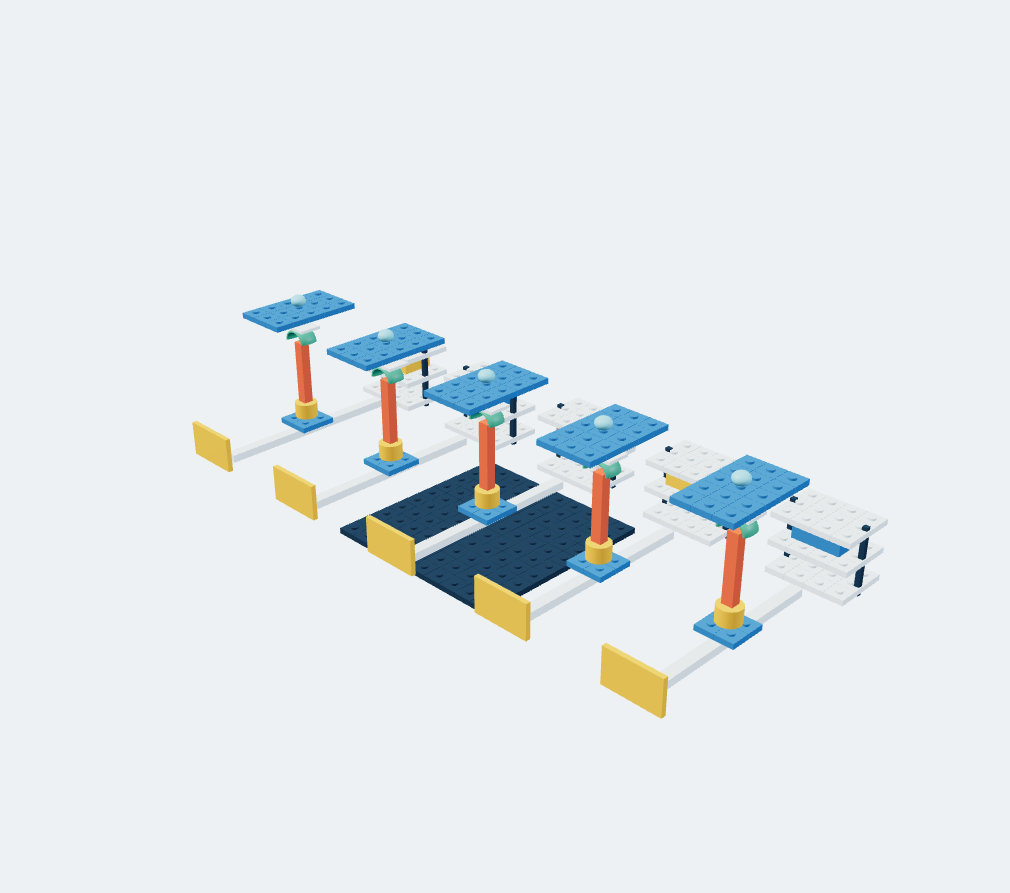
\includegraphics[width=.24\textwidth]{figures/hierarchy3/segmented-antenna-yard-iso.png}
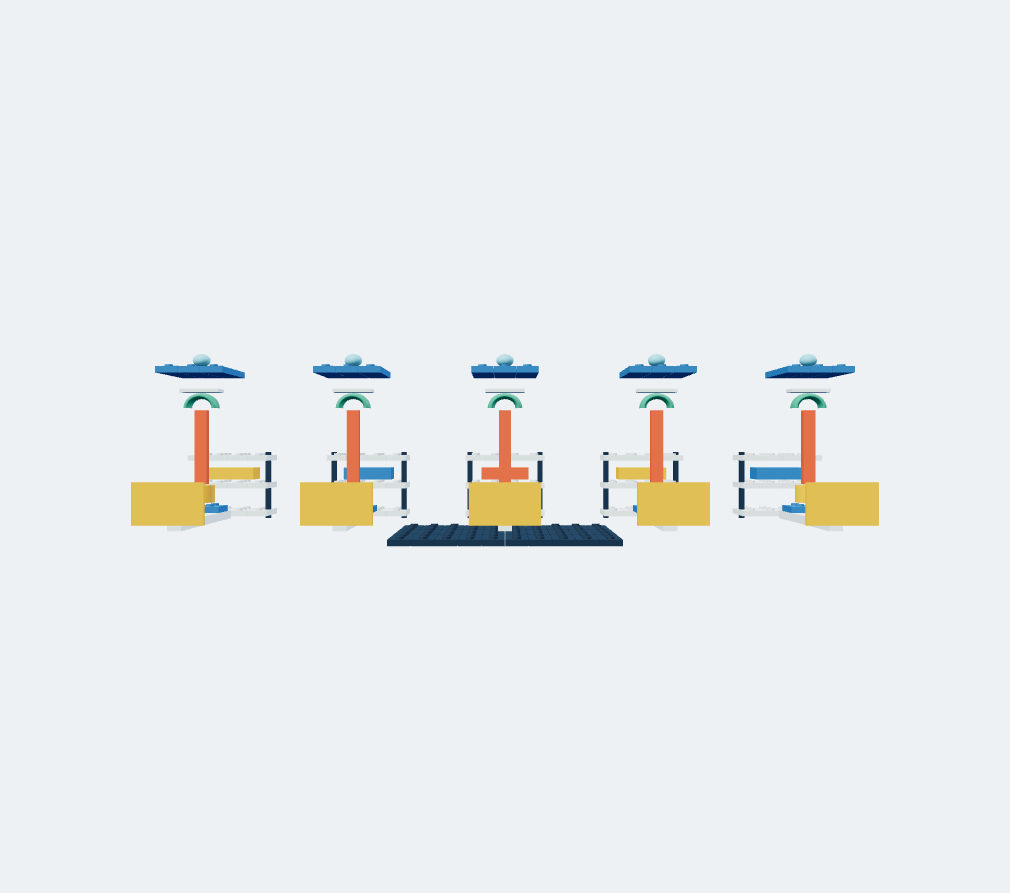
\includegraphics[width=.24\textwidth]{figures/hierarchy3/segmented-antenna-yard-front.png}
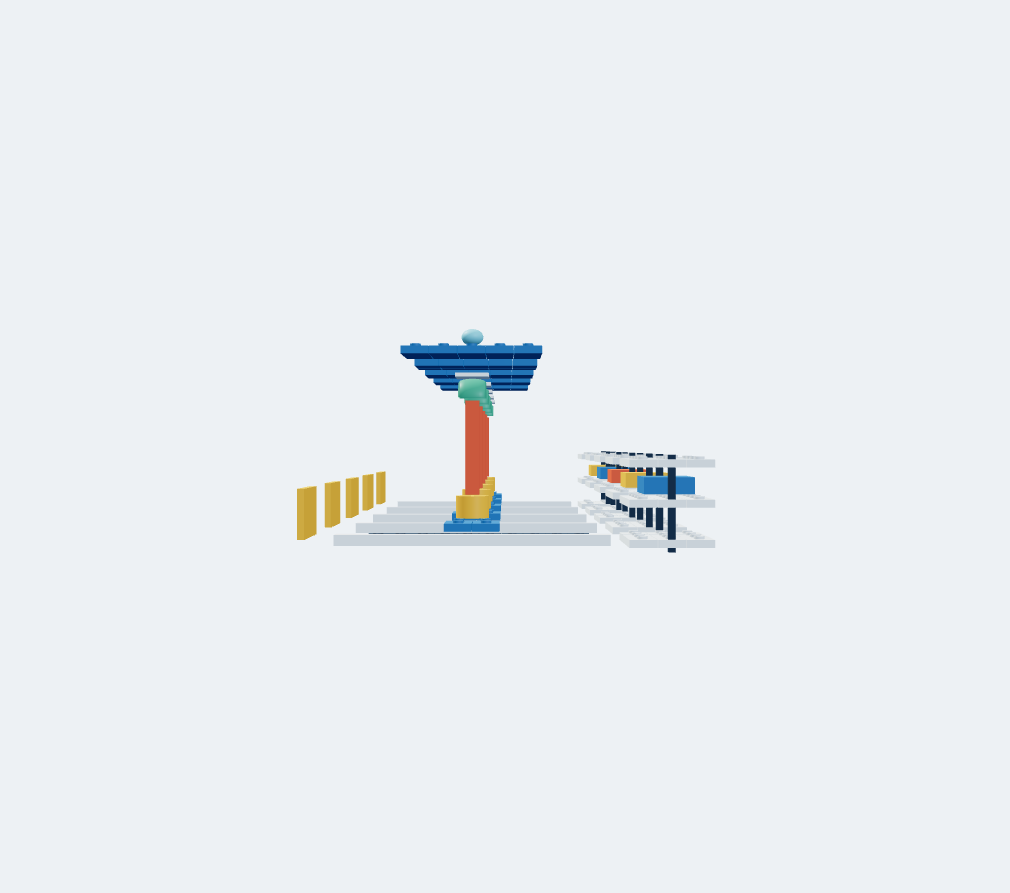
\includegraphics[width=.24\textwidth]{figures/hierarchy3/segmented-antenna-yard-side.png}
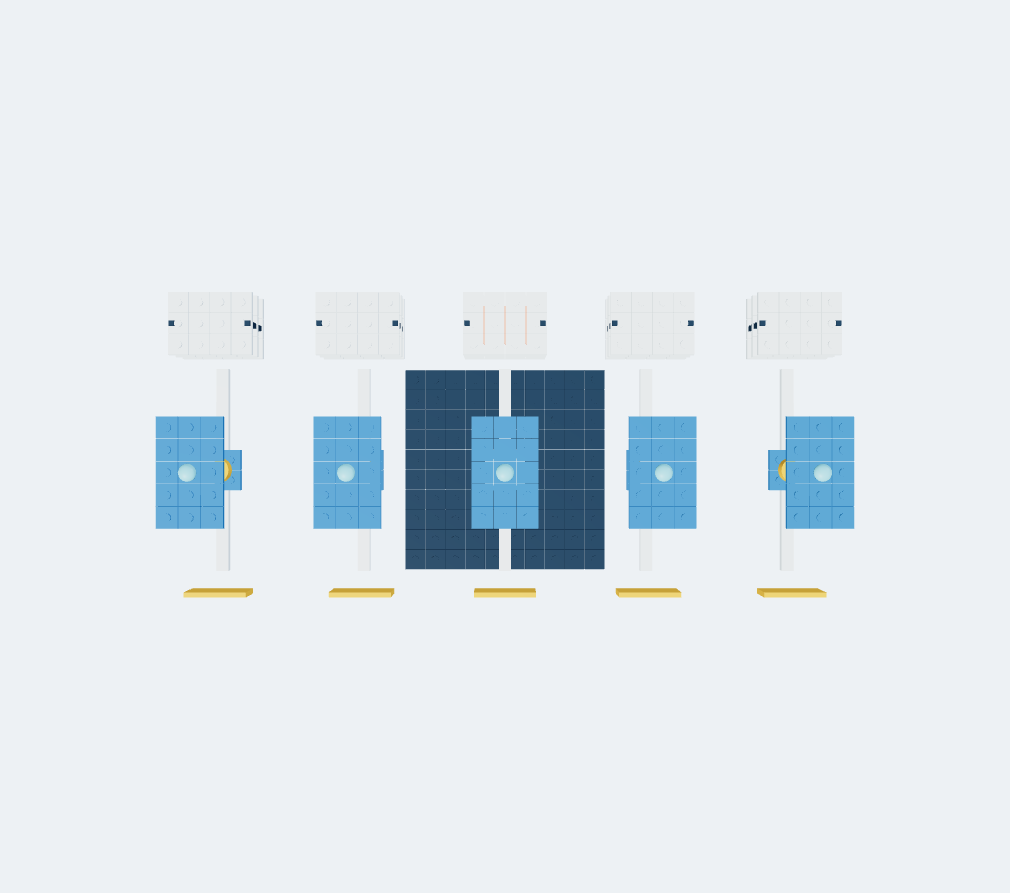
\includegraphics[width=.24\textwidth]{figures/hierarchy3/segmented-antenna-yard-top.png}
\end{center}
\noindent All 48 tasks share this source; complete inputs, choices and answers are in the companion question bank.
\begin{center}\tiny\begin{tabular}{rllll}\toprule No. & Family & Layer & Output & Evidence\\\midrule
1 & identify & atomic & single-choice & model-state \\
2 & count & atomic & single-choice & model-state \\
3 & color & atomic & single-choice & model-state \\
4 & position & atomic & single-choice & model-state \\
5 & joint-type & atomic & single-choice & model-state \\
6 & parent & atomic & single-choice & model-state \\
7 & anchor & atomic & single-choice & model-state \\
8 & degree & atomic & single-choice & model-state \\
9 & recolor & atomic & single-choice & model-state \\
10 & add & atomic & single-choice & model-state \\
11 & remove & atomic & single-choice & model-state \\
12 & replace & atomic & single-choice & model-state \\
13 & translate & atomic & single-choice & model-state \\
14 & rotate & atomic & single-choice & model-state \\
15 & next-module & atomic & single-choice & model-state \\
16 & inventory & atomic & single-choice & model-state \\
17 & boundary & atomic & single-choice & model-state \\
18 & no-op & atomic & single-choice & model-state \\
19 & prefix & metacognitive & single-choice & support-graph \\
20 & access & metacognitive & multiple-choice & Rapier \\
21 & counterfactual & metacognitive & single-choice & support-graph \\
22 & dynamic & metacognitive & single-choice & Rapier \\
23 & kinematic & metacognitive & multiple-choice & model-state \\
24 & diagnosis & metacognitive & multiple-choice & model-state \\
25 & information-gain & metacognitive & multiple-choice & finite-world \\
26 & abstention & metacognitive & single-choice & finite-world \\
27 & posterior & metacognitive & single-choice & finite-world \\
28 & pareto & metacognitive & multiple-choice & model-state \\
29 & assembly & procedural & actions & state-machine \\
30 & disassembly & procedural & actions & state-machine \\
31 & service-repair & procedural & actions & state-machine \\
32 & compound-edit & procedural & actions & state-machine \\
33 & multi-fault & integrative & actions & state-machine \\
34 & scheduling & integrative & schedule & resource-schedule \\
35 & policy & integrative & policy & finite-world \\
36 & local-frame & atomic & single-choice & model-state \\
37 & projection & atomic & single-choice & model-state \\
38 & relative-order & atomic & single-choice & model-state \\
39 & joint-axis & atomic & single-choice & model-state \\
40 & clearance-margin & metacognitive & single-choice & model-state \\
41 & load-moment & metacognitive & single-choice & model-state \\
42 & weighted-posterior & metacognitive & single-choice & finite-world \\
43 & expected-loss & metacognitive & single-choice & finite-world \\
44 & trace-threshold & metacognitive & single-choice & Rapier \\
45 & guarded-repair & procedural & actions & state-machine \\
46 & rollback & procedural & actions & state-machine \\
47 & resource-repair & integrative & actions & state-machine \\
48 & budget-policy & integrative & policy & finite-world \\
\bottomrule\end{tabular}\end{center}
\clearpage
\subsection{48. Tidal Energy Station (D4)}
287 visible parts, 18 modules, 17 joints. Nominal representative-point displacement: 0.0173; angular displacement: 0.0026 rad. No inter-module penetration above 0.005, including directly joined modules.
\begin{center}

\includegraphics[width=.24\textwidth]{figures/hierarchy3/tidal-energy-station-iso.png}

\includegraphics[width=.24\textwidth]{figures/hierarchy3/tidal-energy-station-front.png}

\includegraphics[width=.24\textwidth]{figures/hierarchy3/tidal-energy-station-side.png}

\includegraphics[width=.24\textwidth]{figures/hierarchy3/tidal-energy-station-top.png}
\end{center}
\noindent All 48 tasks share this source; complete inputs, choices and answers are in the companion question bank.
\begin{center}\tiny\begin{tabular}{rllll}\toprule No. & Family & Layer & Output & Evidence\\\midrule
1 & identify & atomic & single-choice & model-state \\
2 & count & atomic & single-choice & model-state \\
3 & color & atomic & single-choice & model-state \\
4 & position & atomic & single-choice & model-state \\
5 & joint-type & atomic & single-choice & model-state \\
6 & parent & atomic & single-choice & model-state \\
7 & anchor & atomic & single-choice & model-state \\
8 & degree & atomic & single-choice & model-state \\
9 & recolor & atomic & single-choice & model-state \\
10 & add & atomic & single-choice & model-state \\
11 & remove & atomic & single-choice & model-state \\
12 & replace & atomic & single-choice & model-state \\
13 & translate & atomic & single-choice & model-state \\
14 & rotate & atomic & single-choice & model-state \\
15 & next-module & atomic & single-choice & model-state \\
16 & inventory & atomic & single-choice & model-state \\
17 & boundary & atomic & single-choice & model-state \\
18 & no-op & atomic & single-choice & model-state \\
19 & prefix & metacognitive & single-choice & support-graph \\
20 & access & metacognitive & multiple-choice & Rapier \\
21 & counterfactual & metacognitive & single-choice & support-graph \\
22 & dynamic & metacognitive & single-choice & Rapier \\
23 & kinematic & metacognitive & multiple-choice & model-state \\
24 & diagnosis & metacognitive & multiple-choice & model-state \\
25 & information-gain & metacognitive & multiple-choice & finite-world \\
26 & abstention & metacognitive & single-choice & finite-world \\
27 & posterior & metacognitive & single-choice & finite-world \\
28 & pareto & metacognitive & multiple-choice & model-state \\
29 & assembly & procedural & actions & state-machine \\
30 & disassembly & procedural & actions & state-machine \\
31 & service-repair & procedural & actions & state-machine \\
32 & compound-edit & procedural & actions & state-machine \\
33 & multi-fault & integrative & actions & state-machine \\
34 & scheduling & integrative & schedule & resource-schedule \\
35 & policy & integrative & policy & finite-world \\
36 & local-frame & atomic & single-choice & model-state \\
37 & projection & atomic & single-choice & model-state \\
38 & relative-order & atomic & single-choice & model-state \\
39 & joint-axis & atomic & single-choice & model-state \\
40 & clearance-margin & metacognitive & single-choice & model-state \\
41 & load-moment & metacognitive & single-choice & model-state \\
42 & weighted-posterior & metacognitive & single-choice & finite-world \\
43 & expected-loss & metacognitive & single-choice & finite-world \\
44 & trace-threshold & metacognitive & single-choice & Rapier \\
45 & guarded-repair & procedural & actions & state-machine \\
46 & rollback & procedural & actions & state-machine \\
47 & resource-repair & integrative & actions & state-machine \\
48 & budget-policy & integrative & policy & finite-world \\
\bottomrule\end{tabular}\end{center}
